\documentclass[12pt,oneside]{report}

\usepackage[T1]{fontenc}
\usepackage{amsmath,amssymb,amsthm}
\usepackage{booktabs}
\usepackage{graphicx}
\usepackage[hidelinks]{hyperref}

\setlength{\emergencystretch}{3em}

\newtheorem{theorem}{Theorem}[chapter]
\newtheorem{proposition}[theorem]{Proposition}
\newtheorem{lemma}[theorem]{Lemma}
\theoremstyle{definition}
\newtheorem{assumption}[theorem]{Assumption}
\theoremstyle{remark}
\newtheorem{remark}[theorem]{Remark}

\newcommand{\notechapter}[2]{%
  \chapter*{Note #1: #2}%
  \addcontentsline{toc}{chapter}{Note #1: #2}%
  \markboth{Note #1: #2}{Note #1: #2}%
  \setcounter{equation}{0}%
  \renewcommand{\theequation}{N#1.\arabic{equation}}%
  \renewcommand{\theHequation}{note.#1.\arabic{equation}}%
}

\title{From Kohn--Sham Density-Functional Theory\\to Effective-Mass Models}
\author{Eugene Joseph M. Ragasa\\
\normalsize Department of Physics, De La Salle University\\
\normalsize 2401 Taft Avenue, Manila 0922, Philippines}
\date{Working research monograph}

\begin{document}

\hypersetup{pageanchor=false}
\pagenumbering{gobble}
\maketitle

\begin{abstract}
This research monograph develops a framework for constructing and evaluating
reduced semiconductor Hamiltonians from first-principles Kohn--Sham
calculations. The initial program considers pristine silicon and substitutional
phosphorus and boron, with representations progressing from periodic
Kohn--Sham operators through Wannier and tight-binding descriptions to lattice
and continuum effective-mass models. It also develops structured learning as a
proposed diagnostic for comparing nested reduced-operator model classes rather
than as a replacement for the first-principles parent. The account distinguishes
physical models, mathematical operators, finite matrix representations, and
software artifacts;
requires common-space, gauge, geometry, spin, unit, and energy-reference
alignment before operator subtraction; and separates spectral fidelity from
aligned-operator fidelity. A coordinated proof program records finite-dimensional
operator identities, alignment and reduction obligations, analytical bounds,
and their mechanization status. It also distinguishes mathematical proof,
software verification, numerical verification, scientific validation, and
uncertainty quantification. At the evidence boundary represented by this draft,
the project has an accepted
represented-operator software foundation, one frozen operator contract checked
by a pinned Lean backend, and retained tutorial and bootstrap execution
observations, but no cross-checked proof package, accepted production bulk
parent, Wannier operator, reduced impurity operator, or continuum crossover. The
document is a
working research monograph, not an institutionally registered dissertation,
submitted manuscript, or completed scientific result.
\end{abstract}

\clearpage
\hypersetup{pageanchor=true}
\pagenumbering{roman}
\chapter*{Preface}
\addcontentsline{toc}{chapter}{Preface}
\markboth{Preface}{Preface}

\chapterstatus{working research monograph with completed synthetic numerical
verification and a proposed material program. No material validation is
claimed.}

This research monograph is a long-form working account of the
\texttt{ksdft2effmass} research program. It is not an institutionally
registered dissertation or a submitted manuscript. It combines accepted
synthetic software and numerical verification with proposed production and
material work. Its purpose is to develop one coherent narrative while
preserving the narrower scopes of articles, conference contributions, software
records, and computational evidence.

\section*{Research assistance and responsibility}
\index{artificial intelligence!research assistance}
\index{scientific rigor}


Large language models assisted with drafting, code development, analysis, and
editorial work. Their outputs were treated as provisional and evaluated under
the same source, verification, provenance, and evidentiary requirements as
other contributions. Scientific claims in this monograph rely on identified
literature and retained calculation or proof records rather than on the use of
an AI system. Responsibility for the selection, interpretation, and reporting
of the material remains with the author.

\clearpage
\section*{Audience}
\index{audience}
\index{pedagogy}


Although this research interest began with the development of a pedagogical
problem, I recognize the breadth of the resulting work. This manuscript serves
partly as a laboratory notebook and partly as a structured set of research
notes. It is intended to help advanced physics undergraduates and graduate
students understand the quantum-mechanical, solid-state, semiconductor,
computational, and mathematical concepts involved in the program.

The manuscript therefore includes a range of exercises developed to move a
reader from reading, through note-taking and computation, and ultimately toward
research. These exercises do not all carry the same evidentiary status. A
pedagogical derivation, controlled numerical experiment, proposed computational
workflow, and retained scientific calculation must remain distinguishable even
when they appear in one continuous narrative.

\section*{How to read the monograph}

The main narrative has four parts. Part~I asks what makes a reduced model
adequate and states the comparison and evidence rules used throughout the
book. Part~II develops the pristine bulk-silicon representation program, from
the first-principles parent through retained and localized representations to
bulk reduced-model selection. Part~III develops the phosphorus and boron
branches, aligned impurity extraction, lattice and continuum model classes,
and transferability questions. Part~IV collects the mathematical and proof
program needed to support the preceding scientific claims. The concluding
chapter then restates the dependency-ordered research sequence.

The appendices form a reference and analytical workbench. They contain detailed
notation, operator geometry, controlled finite-dimensional examples, reduction
route comparisons, completed one- and two-dimensional periodic benchmarks,
completed spin-space and one-dimensional defect benchmarks, a proposed
two-dimensional defect program, and a dedicated envelope-theory appendix
extracting the Luttinger--Kohn, Burt, and Ermoneit equations for the project.
They support the main argument while preserving the distinctions among
synthetic verification, literature analysis, proposed work, and material
validation.

\section*{Status and provenance}

The monograph explains the research program and reports evidence through
identified sources and retained records. Statements about future work are
proposals rather than results. A typeset formula is not by itself a proof, a
proof sketch is not a completed proof, a successful software test is not
scientific validation, and a generated figure is not a calculated result unless
its input, method, software environment, and provenance are identified. When a
calculation, source, or proof record changes the supported interpretation, the
narrative must be updated rather than treated as independent authority.

\section*{Objects kept distinct}

The discussion uses four related but noninterchangeable levels:

\begin{description}
  \item[Physical model.] The chosen description of the material system and its
    physical assumptions, including the Kohn--Sham parent problem and the
    substitutional-impurity branches.
  \item[Mathematical operator.] A map acting between identified state spaces,
    with a stated domain and codomain when these are material to the argument.
  \item[Finite representation.] A matrix obtained only after selecting finite
    subspaces, bases, ordering conventions, units, geometry, gauge, and energy
    reference.
  \item[Software artifact.] An implementation, serialized record, input file,
    workflow, or test that constructs or evaluates a representation.
\end{description}

Equality or subtraction at one level does not automatically define equality or
subtraction at another. In particular, pristine and doped matrices cannot be
subtracted meaningfully until their represented spaces and conventions have
been aligned.

\section*{Evidence vocabulary}
\index{evidence!vocabulary}


The monograph uses explicit status labels:

\begin{description}
  \item[Calculated result.] Produced by an identified calculation with retained
    provenance.
  \item[Literature value.] Taken from an identified and verified source.
  \item[Expected behavior.] A prediction or expectation that has not yet been
    observed in the project.
  \item[Illustrative example.] Explanatory material that is not research
    evidence.
  \item[Synthetic test data.] Constructed data used to verify software behavior,
    not output from a physical calculation.
  \item[Placeholder.] Material awaiting authoritative content or verification.
  \item[Proposed work.] Planned activity that has not been completed.
\end{description}

Chapter-level status statements apply to the prose that follows unless a more
specific label overrides them. Results chapters will identify their retained
sources rather than relying on narrative confidence or visual plausibility.

\section*{Error categories}
\index{error!categories}


Three error sources remain separate throughout the monograph. Parent-model
error concerns the difference between the selected physical parent and an
independent physical reference such as experiment or a higher-level theory.
Numerical or discretization error concerns approximation of the stated parent
mathematics by finite cutoffs, meshes, cells, stencils, and solver tolerances.
Model-reduction error concerns the loss incurred when replacing an aligned
parent representation by a reduced model class. These categories will not be
combined unless a later owning specification establishes compatible definitions
and a valid mathematical relationship among them.

\section*{Program scope}

The initial material system is silicon in the diamond structure. The declared
impurity branches are substitutional phosphorus and substitutional boron in
silicon. Quantum ESPRESSO remains responsible for electronic-structure
calculations, and Wannier90 remains responsible for Wannier localization. The
software in this repository begins from their retained outputs and addresses
representation, alignment, operator extraction, model reduction, evaluation,
and provenance.

The immediate bulk pilot and the later impurity program are related but not
identical scopes. Bulk development does not establish dopant results. Likewise,
a neutral periodic dopant supercell is not silently reinterpreted as an isolated
or ionized impurity. Each such interpretation requires its own declared branch
and evidence.

\citationtodo{medium priority}{Check the periodic-supercell versus isolated- or
ionized-impurity warning against a standard defect-physics source. Candidate:
Freysoldt et al. (2014), bibliography key \texttt{freysoldt2014} (already
present).}

\section*{Relationship to shorter publications}

Articles and presentations may select a narrower question, reorganize the
exposition, and adopt venue-specific terminology. Each publication must still
identify the evidence it uses and preserve the corresponding status,
provenance, and limitations. This monograph remains the broader working account
rather than evidence that any shorter publication has been reviewed or
accepted.

\tableofcontents
\clearpage
\pagenumbering{arabic}

\chapter[From Bloch Waves to Effective-Mass Theory]{From Bloch Waves to
Effective-Mass Theory: A Controlled Atomistic-to-Continuum Framework for
Semiconductor Physics}
\label{ch:operator-reduction-motivation}

\textbf{Status: conceptual and illustrative framework. The central hypothesis,
continuum criteria, and intellectual contributions are proposed work; the
particle-in-a-box example is not research evidence or a validated reduction of
silicon.}

\section{Project motivation and significance}

Semiconductor physics is commonly taught through two quantum-mechanical
descriptions that are physically related but mathematically disconnected.
Students first solve a microscopic periodic Hamiltonian,
\begin{equation}
    \hat H_{\mathrm{micro}}
    =
    -\frac{\hbar^2}{2m_0}\nabla^2
    +
    V_{\mathrm{per}}(\mathbf r),
\end{equation}
and obtain Bloch states and energy bands. They are later introduced to
effective-mass theory through a continuum envelope Hamiltonian. Written
relative to the selected band-edge energy, it is
\begin{equation}
    \hat H_{\mathrm{EMT}}
    =
    -\frac{\hbar^2}{2}
    \nabla\mathbin{\cdot}\mathbf m^{*-1}\nabla
    +
    V_{\mathrm{ext}}(\mathbf r).
\end{equation}

For a smooth, nondegenerate band near an extremum $\mathbf k_0$, the usual
connection expands the dispersion as
\begin{equation}
    E_n(\mathbf k_0+\mathbf q)
    =
    E_n(\mathbf k_0)
    +
    \frac{\hbar^2}{2}
    \mathbf q^{\mathsf T}\mathbf m_n^{*-1}\mathbf q
    +
    O\!\left(\lVert\mathbf q\rVert^3\right).
\end{equation}
After subtracting the constant $E_n(\mathbf k_0)\hat I$ and replacing
$\mathbf q$ by $-i\nabla$, this argument explains the form of the effective
kinetic operator. It does not construct the envelope-function state space,
define the map from microscopic Bloch states to continuum states, or quantify
the approximations introduced by band truncation, gauge selection, valley
decomposition, and spatial coarse-graining.

Effective-mass theory is therefore often presented as a second quantum
mechanics rather than as a controlled reduction of the first. The
effective-mass tensor is obtained from the curvature of a Bloch band, but the
corresponding state-space reduction is usually left implicit.

This project began from a practical attempt to close that pedagogical gap. The
initial objective was to construct an explicit periodic potential that students
could discretize and diagonalize, yet which remained sufficiently expressive
to produce an indirect band gap. Such a model would provide an executable
bridge between elementary periodic quantum mechanics and the band structure of
an indirect-gap semiconductor.

The most direct strategy appears elementary: calculate Kohn--Sham
density-functional-theory Bloch eigenpairs, reconstruct a retained Hamiltonian,
subtract the known kinetic operator, and interpret the remainder as an
effective periodic potential.

Let $\hat H_{\mathrm{KS}}(\mathbf k)$ be a Kohn--Sham Bloch-fiber operator
with cell-periodic eigenstates $\lvert u_{n\mathbf k}\rangle$. For a retained
set of bands $\mathcal B$, define
\begin{equation}
    \hat P(\mathbf k)
    =
    \sum_{n\in\mathcal B}
    \lvert u_{n\mathbf k}\rangle
    \langle u_{n\mathbf k}\rvert
\end{equation}
and
\begin{equation}
    \hat H_{\mathrm{KS}}^{(P)}(\mathbf k)
    =
    \left.
        \hat P(\mathbf k)
        \hat H_{\mathrm{KS}}(\mathbf k)
        \hat P(\mathbf k)
    \right|_{\mathcal H^{(P)}(\mathbf k)}
    =
    \sum_{n\in\mathcal B}
    \varepsilon_n(\mathbf k)
    \lvert u_{n\mathbf k}\rangle
    \langle u_{n\mathbf k}\rvert,
\end{equation}
where
\begin{equation}
    \mathcal H^{(P)}(\mathbf k)
    =
    \operatorname{Ran}\hat P(\mathbf k).
\end{equation}
For entangled bands, constructing a smooth retained family may require
projection or disentanglement rather than selection by a single global energy
cutoff.

The apparently obvious construction is
\begin{equation}
    \hat V_{\mathrm{eff}}^{(P)}(\mathbf k)
    \stackrel{?}{=}
    \hat H_{\mathrm{KS}}^{(P)}(\mathbf k)
    -
    \hat T^{(P)}(\mathbf k),
\end{equation}
where
\begin{equation}
    \hat T^{(P)}(\mathbf k)
    =
    \left.
        \hat P(\mathbf k)
        \hat T(\mathbf k)
        \hat P(\mathbf k)
    \right|_{\mathcal H^{(P)}(\mathbf k)}.
\end{equation}
This subtraction is mathematically valid on the retained fiber, but its result
is a projected operator, not necessarily a unique local scalar potential.
Projection may induce nonlocality, while nonlocal pseudopotentials, orbital
structure, spin--orbit interactions, and band truncation may introduce
components that cannot be represented by a simple function $V(\mathbf r)$.
Bloch gauge freedom further changes the matrix coordinates of the retained
operator without changing its abstract action or spectrum.

The desired teaching potential must therefore be obtained by reducing the
operator residual into an explicitly chosen model class:
\begin{equation}
    \hat V_{\mathrm{teach}}
    =
    \operatorname*{arg\,min}_{\hat V\in\mathcal V_{\mathrm{adm}}}
    \sum_{\mathbf k\in\mathcal K}
    \left\|
        \hat H_{\mathrm{KS}}^{(P)}(\mathbf k)
        -
        \hat T^{(P)}(\mathbf k)
        -
        \left.
            \hat P(\mathbf k)
            \hat V(\mathbf k)
            \hat P(\mathbf k)
        \right|_{\mathcal H^{(P)}(\mathbf k)}
    \right\|_*^2.
\end{equation}
Here, $\mathcal K$ is the sampled reciprocal-space region and
$\mathcal V_{\mathrm{adm}}$ may represent local periodic potentials, truncated
Fourier expansions, finite real-space stencils, or constrained tight-binding
operator classes. The norm $\lVert\cdot\rVert_*$ and any reciprocal-space
weights must be chosen to measure operator error consistently with the physical
observables and continuum limit of interest. This is a proposed model-class
problem, not a presently accepted fitting criterion.

The finite example developed next separates exact operator retention from
model-class approximation and shows why all components of an additive
Hamiltonian must be reduced through the same map. The later sections then
return to pristine--doped comparison, continuum admissibility, and the broader
research program.

\section{From spectral data to an effective Hamiltonian}

The construction in this section is a pedagogical discrete-spectrum case. It
is not the literal subspace construction used for a periodic crystal, where
Bloch-fiber representations and possibly projection or disentanglement enter.

The genesis of this problem begins with the spectral problem for a quantum
Hamiltonian $\hat H$,
\begin{equation}
    \hat H\lvert\psi_i\rangle
    =
    E_i\lvert\psi_i\rangle,
\end{equation}
where $(E_i,\lvert\psi_i\rangle)$ is the $i$th eigenpair. Assuming that the
relevant spectrum is discrete and that the eigenstates form a complete
orthonormal basis of the Hilbert space $\mathcal H$, the Hamiltonian admits the
spectral decomposition
\begin{equation}
    \hat H
    =
    \sum_i
    E_i\lvert\psi_i\rangle\langle\psi_i\rvert.
\end{equation}

Suppose that the physical questions of interest involve only states below an
energy cutoff $E_{\mathrm{cut}}$. We define the retained low-energy subspace
\begin{equation}
    \mathcal H^{(P)}
    =
    \operatorname{span}
    \left\{
        \lvert\psi_i\rangle
        \;\middle|\;
        E_i\leq E_{\mathrm{cut}}
    \right\},
\end{equation}
with orthogonal projector
\begin{equation}
    \hat P
    =
    \sum_{E_i\leq E_{\mathrm{cut}}}
    \lvert\psi_i\rangle\langle\psi_i\rvert.
\end{equation}

The corresponding retained Hamiltonian is
\begin{equation}
    \hat H^{(P)}
    =
    \left.
        \hat P\hat H\hat P
    \right|_{\mathcal H^{(P)}}
    =
    \sum_{E_i\leq E_{\mathrm{cut}}}
    E_i\lvert\psi_i\rangle\langle\psi_i\rvert.
\end{equation}
It exactly reproduces every retained eigenpair,
\begin{equation}
    \hat H^{(P)}\lvert\psi_i\rangle
    =
    E_i\lvert\psi_i\rangle,
    \qquad
    E_i\leq E_{\mathrm{cut}},
\end{equation}
but it does not specify the action of $\hat H$ outside
$\mathcal H^{(P)}$. It is therefore an exact restriction of the parent
Hamiltonian, not yet an approximate effective model.

We reserve the notation $\hat H_{\mathrm{eff}}(\boldsymbol\theta)$ for an
operator belonging to a prescribed effective-model class with parameters
$\boldsymbol\theta$. The distinction is important:
\begin{equation}
    \underbrace{\hat H^{(P)}}_{\text{exact retained operator}}
    \qquad\text{and}\qquad
    \underbrace{\hat H_{\mathrm{eff}}(\boldsymbol\theta)}_{
        \text{approximate model on an identified retained space}}
\end{equation}
are not the same construction.

\section{Computational example: a particle in a one-dimensional box}

The particle in a one-dimensional box provides the simplest computational
setting in which the continuous operator, its discrete matrix representation,
its retained subspace, and an effective model can be separated explicitly.

\subsection{Continuous problem}

Consider a particle of mass $m$ confined to the interval
\begin{equation}
    \Omega=(0,L).
\end{equation}
Inside the box, the Hamiltonian is
\begin{equation}
    \hat H
    =
    -\frac{\hbar^2}{2m}\frac{d^2}{dx^2},
\end{equation}
with operator domain
\begin{equation}
    \mathcal D(\hat H)
    =
    H^2(0,L)\cap H_0^1(0,L).
\end{equation}
Equivalently, the wavefunction satisfies the Dirichlet boundary conditions
\begin{equation}
    \psi(0)=\psi(L)=0.
\end{equation}

The exact eigenfunctions and eigenvalues are
\begin{align}
    \psi_n(x)
    &=
    \sqrt{\frac{2}{L}}
    \sin\left(\frac{n\pi x}{L}\right),
    \\
    E_n
    &=
    \frac{\hbar^2\pi^2n^2}{2mL^2},
    \qquad n=1,2,\ldots.
\end{align}

\subsection{Finite-difference representation}

Introduce $N$ interior grid points
\begin{equation}
    x_j=j\Delta x,
    \qquad
    j=1,\ldots,N,
\end{equation}
where
\begin{equation}
    \Delta x=\frac{L}{N+1}.
\end{equation}
The boundary points are excluded from the numerical state vector because the
Dirichlet conditions fix their values to zero. A sampled wavefunction is
represented by
\begin{equation}
    \boldsymbol\psi
    =
    \begin{bmatrix}
        \psi(x_1) & \psi(x_2) & \cdots & \psi(x_N)
    \end{bmatrix}^{\mathsf T}
    \in\mathbb C^N.
\end{equation}

Using the centered finite-difference approximation
\begin{equation}
    \left.
        \frac{d^2\psi}{dx^2}
    \right|_{x=x_j}
    \approx
    \frac{
        \psi(x_{j+1})-2\psi(x_j)+\psi(x_{j-1})
    }{\Delta x^2},
\end{equation}
the Hamiltonian is represented by the Hermitian matrix
\begin{equation}
    \mathbf H
    =
    \frac{\hbar^2}{2m\Delta x^2}
    \begin{bmatrix}
        2  & -1 & 0  & \cdots & 0 \\
        -1 & 2  & -1 & \ddots & \vdots \\
        0  & -1 & 2  & \ddots & 0 \\
        \vdots & \ddots & \ddots & \ddots & -1 \\
        0 & \cdots & 0 & -1 & 2
    \end{bmatrix}.
\end{equation}

The discrete eigenvalue problem is
\begin{equation}
    \mathbf H\mathbf v_i
    =
    \varepsilon_i\mathbf v_i,
\end{equation}
where $\varepsilon_i$ approximates $E_i$. With Euclidean normalization,
$\mathbf v_i$ approximates the quadrature-scaled samples
$\sqrt{\Delta x}\,\psi_i(x_j)$ rather than the unscaled samples themselves.
The finite-difference eigenvalues are
\begin{equation}
    \varepsilon_i
    =
    \frac{2\hbar^2}{m\Delta x^2}
    \sin^2\left(
        \frac{i\pi}{2(N+1)}
    \right),
    \qquad i=1,\ldots,N.
\end{equation}
For fixed $i$,
\begin{equation}
    \lim_{\Delta x\rightarrow 0}\varepsilon_i
    =
    E_i.
\end{equation}
The low-energy eigenpairs converge first because their wavelengths remain
large compared with the grid spacing. States near the grid-resolution limit
are strongly affected by the finite-difference dispersion relation.

\subsection{Spectral reconstruction in the discrete space}

Let
\begin{equation}
    \boldsymbol\Phi
    =
    \begin{bmatrix}
        \mathbf v_1 & \mathbf v_2 & \cdots & \mathbf v_N
    \end{bmatrix}
\end{equation}
be the unitary eigenvector matrix and let
\begin{equation}
    \boldsymbol\Lambda
    =
    \operatorname{diag}
    \left(
        \varepsilon_1,\ldots,\varepsilon_N
    \right).
\end{equation}
Then
\begin{equation}
    \boldsymbol\Phi^\dagger\boldsymbol\Phi
    =
    \mathbf I,
\end{equation}
and the discrete Hamiltonian can be reconstructed exactly as
\begin{equation}
    \mathbf H
    =
    \boldsymbol\Phi
    \boldsymbol\Lambda
    \boldsymbol\Phi^\dagger
    =
    \sum_{i=1}^{N}
    \varepsilon_i\mathbf v_i\mathbf v_i^\dagger.
\end{equation}

The relation between the continuous and discrete objects should therefore be
written as a representation map,
\begin{equation}
    \hat H
    \longrightarrow
    \mathbf H,
\end{equation}
rather than as a literal equality. The matrix $\mathbf H$ depends on the
chosen grid, finite-difference stencil, boundary conditions, and units.

\subsection{Low-energy retention}

Assume $1\leq M<N$. Let
\begin{equation}
    \boldsymbol\Phi_M
    =
    \begin{bmatrix}
        \mathbf v_1 & \mathbf v_2 & \cdots & \mathbf v_M
    \end{bmatrix}
    \in\mathbb C^{N\times M}
\end{equation}
contain the lowest $M$ eigenvectors, and define
\begin{equation}
    \boldsymbol\Lambda_M
    =
    \operatorname{diag}
    \left(
        \varepsilon_1,\ldots,\varepsilon_M
    \right).
\end{equation}
The orthogonal projector onto the retained discrete subspace is
\begin{equation}
    \mathbf P_M
    =
    \boldsymbol\Phi_M\boldsymbol\Phi_M^\dagger.
\end{equation}

The retained Hamiltonian embedded in the original grid space is
\begin{align}
    \mathbf H^{(P_M)}
    &=
    \mathbf P_M\mathbf H\mathbf P_M
    \\
    &=
    \boldsymbol\Phi_M
    \boldsymbol\Lambda_M
    \boldsymbol\Phi_M^\dagger.
\end{align}
This is an $N\times N$ matrix of rank $M$. It represents the exact action of
$\mathbf H$ on $\operatorname{Ran}(\mathbf P_M)$ and vanishes on the
orthogonal complement.

The same retained operator has the $M\times M$ matrix representation
\begin{align}
    \mathbf H_{\mathrm{red}}
    &=
    \boldsymbol\Phi_M^\dagger
    \mathbf H
    \boldsymbol\Phi_M
    \\
    &=
    \boldsymbol\Lambda_M
\end{align}
in the retained eigenbasis. Thus,
\begin{equation}
    \mathbf H^{(P_M)}\in\mathbb C^{N\times N},
    \qquad
    \mathbf H_{\mathrm{red}}\in\mathbb C^{M\times M},
\end{equation}
The two matrices represent the same retained action only after restricting
$\mathbf H^{(P_M)}$ to $\operatorname{Ran}(\mathbf P_M)$ and identifying
$\mathbb C^M$ with that range through $\boldsymbol\Phi_M$.

Consequently, the expression
\begin{equation}
    \mathbf H-\mathbf H_{\mathrm{red}}
\end{equation}
is undefined when $M\neq N$. The reduced matrix must first be embedded into
the grid space,
\begin{equation}
    \mathbf H^{(P_M)}
    =
    \boldsymbol\Phi_M
    \mathbf H_{\mathrm{red}}
    \boldsymbol\Phi_M^\dagger,
\end{equation}
or the full Hamiltonian must be restricted to the retained coordinates.

\subsection{Operator residuals}

The full-grid residual associated with spectral retention is
\begin{align}
    \mathbf R_{\mathrm{full}}
    &=
    \mathbf H-\mathbf H^{(P_M)}
    \\
    &=
    \sum_{i=M+1}^{N}
    \varepsilon_i\mathbf v_i\mathbf v_i^\dagger.
\end{align}
For the positive, increasingly ordered particle-in-a-box spectrum,
\begin{align}
    \left\|\mathbf R_{\mathrm{full}}\right\|_2
    &=
    \varepsilon_N,
    \\
    \left\|\mathbf R_{\mathrm{full}}\right\|_{\mathrm F}
    &=
    \left(
        \sum_{i=M+1}^{N}\varepsilon_i^2
    \right)^{1/2}.
\end{align}
These norms are dominated by the discarded high-energy sector. They do not
measure the accuracy with which the retained low-energy action is reproduced.
Indeed,
\begin{equation}
    \mathbf P_M
    \left(
        \mathbf H-\mathbf H^{(P_M)}
    \right)
    \mathbf P_M
    =
    \mathbf 0.
\end{equation}

Now suppose that
$\mathbf H_{\mathrm{eff}}(\boldsymbol\theta)\in\mathbb C^{M\times M}$ is a
parameterized effective model expressed in the retained basis. Its relevant
operator residual is
\begin{equation}
    \mathbf R_H^{(P_M)}(\boldsymbol\theta)
    =
    \boldsymbol\Phi_M^\dagger
    \mathbf H
    \boldsymbol\Phi_M
    -
    \mathbf H_{\mathrm{eff}}(\boldsymbol\theta).
\end{equation}
A Frobenius-norm fitting problem can then be posed as
\begin{equation}
    \boldsymbol\theta^\star
    =
    \operatorname*{arg\,min}_{\boldsymbol\theta}
    \left\|
        \mathbf R_H^{(P_M)}(\boldsymbol\theta)
    \right\|_{\mathrm F}^2.
\end{equation}
This comparison is well defined because both matrices act on the same
$M$-dimensional state space and use the same retained basis.

\section{Conditions for identifying a reduced potential operator}

A reduced Hamiltonian does not by itself determine a unique kinetic--potential
decomposition. Such an identification requires a prescribed model class and a
specified kinetic operator; projected components may also be nonlocal even
when their parent-space counterparts are local.

Suppose that the parent Hamiltonian admits the additive decomposition
\begin{equation}
    \hat H=\hat T+\hat V,
\end{equation}
where $\hat T$ is the kinetic-energy operator and $\hat V$ is the
potential-energy operator. In the parent state space,
\begin{equation}
    \hat V=\hat H-\hat T.
\end{equation}
After discretization on a common numerical state space, this becomes
\begin{align}
    \mathbf H
    &=
    \mathbf T+\mathbf V,
    \\
    \mathbf V
    &=
    \mathbf H-\mathbf T.
\end{align}

It is tempting to apply the same construction to a reduced Hamiltonian and
write
\begin{equation}
    \mathbf V_{\mathrm{eff}}
    \stackrel{?}{=}
    \mathbf H_{\mathrm{eff}}-\mathbf T.
\end{equation}
This expression is meaningful only if $\mathbf H_{\mathrm{eff}}$ and
$\mathbf T$ act on the same state space and are represented in the same
basis. If the Hamiltonian has been reduced, then the kinetic operator must be
reduced through the same map.

\subsection{Consistent reduction of an additive decomposition}

Define the projection map
\begin{equation}
    \mathcal R_{P_M}(\mathbf A)
    =
    \mathbf P_M\mathbf A\mathbf P_M.
\end{equation}
Because $\mathcal R_{P_M}$ is linear,
\begin{align}
    \mathcal R_{P_M}(\mathbf H)
    &=
    \mathcal R_{P_M}(\mathbf T)
    +
    \mathcal R_{P_M}(\mathbf V),
    \\
    \mathbf H^{(P_M)}
    &=
    \mathbf T^{(P_M)}
    +
    \mathbf V^{(P_M)},
\end{align}
where
\begin{align}
    \mathbf T^{(P_M)}
    &=
    \mathbf P_M\mathbf T\mathbf P_M,
    \\
    \mathbf V^{(P_M)}
    &=
    \mathbf P_M\mathbf V\mathbf P_M.
\end{align}
The retained potential is therefore
\begin{equation}
    \mathbf V^{(P_M)}
    =
    \mathbf H^{(P_M)}
    -
    \mathbf T^{(P_M)},
\end{equation}
not
\begin{equation}
    \mathbf V^{(P_M)}
    \stackrel{?}{=}
    \mathbf H^{(P_M)}-\mathbf T.
\end{equation}

In the retained basis, the same relation is
\begin{align}
    \mathbf H_{\mathrm{red}}
    &=
    \boldsymbol\Phi_M^\dagger
    \mathbf H
    \boldsymbol\Phi_M,
    \\
    \mathbf T_{\mathrm{red}}
    &=
    \boldsymbol\Phi_M^\dagger
    \mathbf T
    \boldsymbol\Phi_M,
    \\
    \mathbf V_{\mathrm{red}}
    &=
    \boldsymbol\Phi_M^\dagger
    \mathbf V
    \boldsymbol\Phi_M,
\end{align}
with
\begin{equation}
    \mathbf V_{\mathrm{red}}
    =
    \mathbf H_{\mathrm{red}}-\mathbf T_{\mathrm{red}}.
\end{equation}

\subsection{The particle-in-a-box counterexample}

For the infinite particle in a box, the interior potential vanishes:
\begin{equation}
    V(x)=0.
\end{equation}
The infinite walls are not represented by finite values of $V(x)$; they are
encoded in the domain of $\hat H$ and its Dirichlet boundary conditions. On
the interior finite-difference grid,
\begin{equation}
    \mathbf H=\mathbf T,
    \qquad
    \mathbf V=\mathbf 0.
\end{equation}
Consistent projection gives
\begin{equation}
    \mathbf H^{(P_M)}
    =
    \mathbf T^{(P_M)},
\end{equation}
and hence
\begin{equation}
    \mathbf V^{(P_M)}
    =
    \mathbf H^{(P_M)}-\mathbf T^{(P_M)}
    =
    \mathbf 0.
\end{equation}

Now subtract the unprojected kinetic matrix instead:
\begin{equation}
    \widetilde{\mathbf V}_{\mathrm{eff}}
    =
    \mathbf H^{(P_M)}-\mathbf T.
\end{equation}
For the particle in the box,
\begin{equation}
    \widetilde{\mathbf V}_{\mathrm{eff}}
    =
    \mathbf P_M\mathbf T\mathbf P_M-\mathbf T.
\end{equation}
Because $\mathbf P_M$ is a spectral projector of $\mathbf T$, it commutes
with $\mathbf T$. Let
\begin{equation}
    \mathbf Q_M=\mathbf I-\mathbf P_M
\end{equation}
project onto the discarded subspace. Then
\begin{align}
    \widetilde{\mathbf V}_{\mathrm{eff}}
    &=
    -\mathbf Q_M\mathbf T\mathbf Q_M
    \\
    &=
    -\sum_{i=M+1}^{N}
    \varepsilon_i\mathbf v_i\mathbf v_i^\dagger.
\end{align}
The reconstructed matrix is nonzero even though the physical potential inside
the box is zero. It is not an effective potential. It is the negative of the
discarded high-energy kinetic operator produced by combining a projected
Hamiltonian with an unprojected kinetic operator.

This counterexample separates two obstructions. Subtracting
$\mathbf H_{\mathrm{red}}$ from the full-grid $\mathbf T$ is undefined because
the matrices act on different spaces. Subtracting $\mathbf H^{(P_M)}$ from
$\mathbf T$ is algebraically defined in the common grid representation, but
the result is not the consistently reduced potential. Physical interpretation
therefore requires both a common representation and a common reduction map.

\subsection{Potential residual}

Let $\mathbf V_{\mathrm{eff}}(\boldsymbol\theta)$ be a proposed effective
potential acting on the retained space. The potential residual is
\begin{equation}
    \mathbf R_V^{(P_M)}(\boldsymbol\theta)
    =
    \mathbf V_{\mathrm{red}}
    -
    \mathbf V_{\mathrm{eff}}(\boldsymbol\theta).
\end{equation}
If
\begin{align}
    \mathbf V_{\mathrm{red}}
    &=
    \mathbf H_{\mathrm{red}}-\mathbf T_{\mathrm{red}},
    \\
    \mathbf V_{\mathrm{eff}}(\boldsymbol\theta)
    &=
    \mathbf H_{\mathrm{eff}}(\boldsymbol\theta)
    -
    \mathbf T_{\mathrm{eff}}(\boldsymbol\theta),
\end{align}
then
\begin{equation}
    \mathbf R_V^{(P_M)}(\boldsymbol\theta)
    =
    \left(
        \mathbf H_{\mathrm{red}}
        -
        \mathbf H_{\mathrm{eff}}(\boldsymbol\theta)
    \right)
    -
    \left(
        \mathbf T_{\mathrm{red}}
        -
        \mathbf T_{\mathrm{eff}}(\boldsymbol\theta)
    \right).
\end{equation}
Only when the kinetic operators have been identified,
\begin{equation}
    \mathbf T_{\mathrm{eff}}(\boldsymbol\theta)
    =
    \mathbf T_{\mathrm{red}},
\end{equation}
does the potential residual reduce to the Hamiltonian residual:
\begin{equation}
    \mathbf R_V^{(P_M)}(\boldsymbol\theta)
    =
    \mathbf H_{\mathrm{red}}
    -
    \mathbf H_{\mathrm{eff}}(\boldsymbol\theta).
\end{equation}

\section{From the particle in a box to electronic-structure reduction}

The particle-in-a-box example is elementary, but the obstruction it reveals is
general. In a common parent state space, the decomposition
\begin{equation}
    \mathbf H=\mathbf T+\mathbf V
\end{equation}
is meaningful because all three matrices act on the same discrete state space
and are represented in the same basis. Reduction preserves this additive
decomposition only when every term is reduced through the same map:
\begin{equation}
    \mathcal R_{P_M}(\mathbf H-\mathbf T)
    =
    \mathcal R_{P_M}(\mathbf H)
    -
    \mathcal R_{P_M}(\mathbf T).
\end{equation}
In general,
\begin{equation}
    \mathcal R_{P_M}(\mathbf H-\mathbf T)
    \neq
    \mathcal R_{P_M}(\mathbf H)-\mathbf T.
\end{equation}

The distinction becomes more consequential in electronic-structure
calculations. A Kohn--Sham Hamiltonian, a Wannier Hamiltonian, a tight-binding
Hamiltonian, and an effective-mass Hamiltonian generally do not begin as
matrices acting on an identical numerical state space. They may differ in
dimension, basis, gauge, spatial resolution, boundary conditions, geometry,
units, and energy reference. Their matrices therefore cannot be physically
compared merely because they are all called Hamiltonians.

The central problem of this work is consequently not the mechanical
subtraction of two matrices. It is the construction and validation of the
state-space identifications that make such a subtraction mathematically
defined and physically interpretable.

\section{From periodic potentials to impurity operators}

The same structural problem becomes more consequential when the model is
extended from bulk bands to semiconductor impurities. Given pristine and doped
Hamiltonians, the natural proposal is
\begin{equation}
    \hat V_{\mathrm{imp}}
    \stackrel{?}{=}
    \hat H_d-\hat H_b.
\end{equation}
This expression is not yet an operator identity because independently
constructed pristine and doped calculations may use different retained
subspaces, Bloch or Wannier gauges, basis orderings, geometries, spin
structures, energy references, and numerical dimensions. Their matrices cannot
be interpreted as representations in common physical coordinates without an
explicit identification.

Let $s\in\{b,d\}$ denote matched bulk and doped branches, with retained
operators
\begin{equation}
    \hat H_s^{(P)}
    =
    \left.
        \hat P_s\hat H_s\hat P_s
    \right|_{\mathcal H_s^{(P)}},
    \qquad
    \mathcal H_s^{(P)}
    =
    \operatorname{Ran}\hat P_s.
\end{equation}
If the retained ranks agree, a meaningful comparison requires an
identification
\begin{equation}
    \hat U_d:
    \mathcal H_b^{(P)}
    \longrightarrow
    \mathcal H_d^{(P)}.
\end{equation}
Let $c_b$ and $c_d$ be the scalar reference energies selected by the declared
alignment procedure, and define
\begin{equation}
    \overline{\hat H}_s^{(P)}
    =
    \hat H_s^{(P)}-c_s\hat I_s.
\end{equation}
For a unitary identification $\hat U_d$, the aligned impurity operator on the
bulk retained space is
\begin{equation}
    \Delta\hat H_d^{(P)}
    =
    \hat U_d^\dagger
    \overline{\hat H}_d^{(P)}
    \hat U_d
    -
    \overline{\hat H}_b^{(P)}.
\end{equation}
Unequal retained ranks require a separately defined partial identification or
further model reduction; they do not admit this unitary formula unchanged.

Equal-dimensional spaces admit many abstract unitary maps. Most are not
physically admissible: an arbitrary unitary can scramble localization, orbital
character, crystal momentum, valley content, symmetry, and spin while leaving
the spectrum unchanged. Gauge alignment is therefore necessary to define the
subtraction, but it is not sufficient to select a physical impurity operator.
The identification must also respect the structures needed by the intended
reduced theory.

\section{Central hypothesis}

The central hypothesis proposed by this project is:
\begin{quote}
\itshape
The intended continuum limit is not merely a downstream approximation to an
already constructed atomistic model. It constrains, from the beginning, the
admissible retained spaces, gauges, identification maps, and reduced operator
classes.
\end{quote}

For a semiconductor representation to support an effective-mass
interpretation, its atomistic-to-continuum identification must preserve or
control the structures used by the continuum theory. These include
\begin{itemize}
    \item real-space localization and lattice translation;
    \item Bloch wave vector and valley correspondence;
    \item orbital, symmetry, and spin content;
    \item smoothness across the relevant reciprocal-space region;
    \item common bulk behavior away from an impurity;
    \item boundary conditions and normalization; and
    \item separation of slowly varying envelopes from lattice-periodic
          components.
\end{itemize}

Let
\begin{equation}
    \epsilon=\frac{a}{L}
\end{equation}
denote the ratio of lattice scale $a$ to an envelope or impurity scale $L$.
For a specified family of retained atomistic operators
$\hat H_\epsilon^{(P)}$ and appropriately normalized identification maps
\begin{equation}
    \hat J_\epsilon:
    \mathcal H_\epsilon^{(P)}
    \longrightarrow
    \mathcal H_{\mathrm{EMT}},
\end{equation}
one possible continuum criterion is norm-resolvent convergence,
\begin{equation}
    \left\|
        \hat J_\epsilon
        \left(\hat H_\epsilon^{(P)}-z\right)^{-1}
        \hat J_\epsilon^\dagger
        -
        \left(\hat H_{\mathrm{EMT}}-z\right)^{-1}
    \right\|
    \longrightarrow 0,
    \qquad
    \epsilon\longrightarrow 0,
\end{equation}
for $z$ in an identified common resolvent set. This is a candidate analytical
form, not an established result of the project. A later specification may
instead require a weaker, explicitly defined combination of spectral,
subspace, operator, and observable convergence criteria.

The continuum limit thereby becomes an upstream admissibility condition. A
gauge, basis, identification, or reduced operator class is acceptable only if
it preserves, or approximates with controlled error, the microscopic structures
needed to recover the declared envelope theory.

\section{Relation to Hilbert's sixth problem}

This research is situated within the broad mathematical tradition associated
with Hilbert's sixth problem: the rigorous formulation of physical theories and
the justification of limiting relations between microscopic and continuum
descriptions. It does not claim to solve Hilbert's sixth problem in its general
form. Instead, it addresses a bounded and experimentally consequential
instance: the reduction of microscopic electronic-structure operators to
continuum envelope models for indirect-gap semiconductors and their impurities.

The relevant limiting process is not only a passage between different length
scales. It is a passage between different state spaces, operator algebras,
coordinate systems, and model classes:
\begin{equation}
    \text{KS--DFT}
    \longrightarrow
    \text{retained Bloch operator}
    \longrightarrow
    \text{localized atomistic operator}
    \longrightarrow
    \text{effective-mass continuum operator}.
\end{equation}
Each arrow requires an explicit map, a statement of preserved structure, and an
error criterion. Without these elements, agreement between selected band
energies does not establish that two models represent the same reduced physics.

The effective-mass limit is therefore both an endpoint and a constraint. The
program asks not only whether an atomistic calculation can reproduce a
continuum observable, but which atomistic representations and reductions are
capable of supporting the continuum theory at all.

\section{Intellectual contribution}

The proposed program aims to develop a gauge-equivariant,
continuum-constrained framework for semiconductor operator reduction. Its
intended contributions are
\begin{enumerate}
    \item reconstruction of retained operators from Kohn--Sham Bloch
          eigenpairs;
    \item separation of operator reconstruction from model-class
          approximation;
    \item quantitative projection onto interpretable periodic-potential,
          stencil, and tight-binding classes;
    \item explicit alignment of pristine and doped retained state spaces;
    \item construction of impurity operators whose abstract action is invariant
          under compatible coordinate changes after alignment;
    \item formulation of continuum-compatibility criteria using operator,
          subspace, spectral, and observable errors; and
    \item an executable pedagogical chain connecting periodic potentials,
          indirect band structure, impurity operators, and effective-mass
          theory.
\end{enumerate}

The conceptual distinction is concise:
\begin{quote}
\itshape
Gauge alignment makes an operator comparison mathematically defined;
continuum compatibility makes the resulting reduced model physically
admissible.
\end{quote}

What began as an attempt to construct a teachable periodic potential therefore
exposes a broader mathematical problem. Obtaining the potential requires
reconstructing an operator rather than merely fitting a spectrum. Introducing
an impurity requires comparing independently constructed operators. Comparing
those operators requires identifying their state spaces and gauges. Selecting
physically admissible identifications and reduced models requires a declared
continuum limit.

This chain provides both the scientific rationale and the educational
significance of the proposed research. It converts the normally implicit
transition from Bloch theory to effective-mass theory into an explicit,
testable, and executable sequence of operator reductions while keeping every
approximation and evidence claim explicit. Chapter~\ref{ch:physical-problem}
next specializes this framework to the silicon host and its substitutional
phosphorus and boron branches.

\chapter{Silicon Host and Dopant Research Questions}
\label{ch:physical-problem}

\textbf{Status: expository synthesis of the accepted physical specification;
research outcomes remain proposed work.}

\section{The parent description}

The program asks when a first-principles Kohn--Sham description of silicon and
substitutional dopants can be replaced by a smaller model without losing the
operator information needed for its declared use. The question is not whether
one model is universally ``correct.'' It is whether a stated reduced-model
class preserves stated features of a stated parent problem within separately
declared errors.

The accepted physical conventions are owned by
\path{specification/ksdft2Effmass.physical-specification.v1.md}. This chapter
organizes those conventions as a research narrative and introduces no new
physical branch.

The parent is a self-consistent Kohn--Sham density-functional calculation in
the Born--Oppenheimer fixed-ion framework~\cite{hohenberg1964,kohn1965}. Its
output is a one-particle Kohn--Sham operator and associated finite numerical
representations. It is not the complete interacting many-body Hamiltonian, and
its eigenvalues are not identified here with the complete many-body excitation
spectrum.

For the version-one program, exchange and correlation are described with the
PBE generalized-gradient approximation~\cite{perdew1996}, and the
electron--ion interaction is represented by compatible optimized
norm-conserving Vanderbilt pseudopotentials from the approved PseudoDojo
family~\cite{hamann2013,vansetten2018}. These choices define the parent against
which later reductions are measured. In particular, disagreement between this
parent and experiment is a parent-model question, not automatically an error
introduced by tight-binding or effective-mass reduction.

\section{Pristine silicon host}

The host is crystalline silicon in the diamond structure: an fcc Bravais
lattice with a two-atom basis. Primitive-cell and conventional-cell
coordinates may both be useful, but every retained representation must
identify which lattice vectors, axes, basis sites, and reciprocal-coordinate
convention it uses.

The immediate bulk pilot is scalar relativistic, non-spin-polarized, and does
not include spin--orbit coupling. Its production lattice constant is to be
obtained from a zero-pressure PBE bulk relaxation using the selected silicon
pseudopotential. Until that calculation and its convergence record exist, no
numerical lattice constant is a calculated result of this project.

The pilot targets a band-edge subspace sufficient for an orthogonal
$sp^3s^{\ast}$ reduction, including the valence and low-conduction states
needed to describe the indirect Kohn--Sham gap and electron effective masses.
The exact band count, projection choices, and Wannier windows belong to later
methodological records. They are not fixed by the phrase ``band-edge
subspace'' alone.

The declared bulk observables are the indirect Kohn--Sham gap, the
conduction-valley position, longitudinal and transverse electron effective
masses, and withheld-point band errors. These quantities serve distinct roles:
they characterize the selected parent, test numerical convergence, and later
evaluate reduced representations. Passing one role does not imply passing the
others.

\section{Compatible host and dopant branches}

Each doped calculation uses a periodic supercell built from the frozen host
lattice vectors, with one substitutional dopant and a matched pristine
comparison supercell. In the primary dopant branches, internal atomic
coordinates are relaxed while the approved bulk lattice vectors remain fixed;
unrelaxed structures are retained only as diagnostics. Geometry and site
correspondence must be identified before pristine and doped operators are
compared.

The immediate non-spin-polarized, non-SOC bulk pilot does not by itself supply
every host reference required by the dopant program. A phosphorus comparison
requires a compatible bulk reference with documented spin and SOC conventions.
Final boron acceptor and continuum claims require a matching fully relativistic,
noncollinear SOC bulk reference. Operators from these different spin spaces are
not directly subtractable without an explicit identification.

\section{Substitutional phosphorus}

The phosphorus branch replaces one silicon atom at a diamond-lattice site by
phosphorus in a periodic supercell. Its primary version-one charge state is
neutral $\mathrm{P}_{\mathrm{Si}}^{0}$. With the accepted pseudopotential
valences, this system has one additional valence electron relative to the
matched pristine silicon supercell and therefore an odd valence-electron count.
The primary branch is consequently scalar relativistic, collinearly spin
polarized, and non-SOC.

The neutral supercell contains both the donor-core perturbation relative to
silicon and the additional electron that occupies and screens that
perturbation. It must not be relabelled silently as an isolated ionized donor.
A charged $\mathrm{P}_{\mathrm{Si}}^{+}$ calculation, or an extraction intended
to isolate an ionized-core potential, requires a separately specified
controlled branch.

The eventual phosphorus questions concern donor energies relative to a
compatible conduction-band reference, valley composition, localization or
envelope diagnostics, and the spatial structure of an aligned impurity
operator. Each finite supercell represents a periodic dopant array. An
isolated-donor interpretation requires supercell-size evidence rather than the
presence of a single substituted atom in the simulation cell.

\section{Substitutional boron}

The boron branch replaces one silicon atom by boron and uses neutral
$\mathrm{B}_{\mathrm{Si}}^{0}$ as its primary version-one charge state. The
accepted valence convention gives one fewer valence electron than in the
matched pristine supercell and again produces an odd electron count.

For final acceptor and continuum claims, the physical specification requires a
fully relativistic, noncollinear spinor calculation with spin--orbit coupling.
A scalar-relativistic non-SOC calculation may be retained only as an explicitly
labelled method-development branch. This distinction prevents an early
simplification from being presented as the final physical treatment of the
spin--orbit-coupled valence manifold.

The eventual boron questions concern acceptor energies relative to a
compatible valence-band reference, valence-subspace fidelity, localization or
envelope diagnostics, and the radial structure of the aligned impurity
operator. Charged $\mathrm{B}_{\mathrm{Si}}^{-}$ calculations are deferred to
a separate controlled branch.

\section{From parent models to reduced models}

The program studies a sequence of representations rather than one direct leap
from density-functional theory to continuum theory:
\begin{enumerate}
    \item a converged Kohn--Sham parent problem;
    \item a retained projected or Wannier subspace;
    \item an aligned finite operator representation;
    \item a constrained lattice model, initially an orthogonal
          $sp^3s^{\ast}$ hierarchy for bulk silicon;
    \item an extracted and reduced impurity operator; and
    \item where justified, a continuum effective-mass description.
\end{enumerate}

Projection, localization, alignment, parameter fitting, truncation, and
continuum approximation are different operations. Their errors and assumptions
must therefore remain identifiable. Wannier localization alone is not a
low-rank approximation, and a good spectral fit alone does not establish
agreement of aligned operator matrix elements.

\section{Research questions}

Within these boundaries, the long-form study is organized by the following
questions:
\begin{enumerate}
    \item Which finite subspace and representation preserve the declared bulk
          Kohn--Sham features with controlled numerical error?
    \item Can a prescribed tight-binding model class satisfy both spectral and
          aligned-operator criteria, and what is the smallest tested class that
          does so?
    \item What basis, gauge, geometry, unit, and energy-reference
          identifications are required before pristine and doped operators can
          be compared?
    \item After those identifications, what portion of the
          substitutional-dopant perturbation can be represented by nested local
          or nonlocal lattice-model classes?
    \item Under separately defined acceptance rules, when does a continuum
          effective-mass description preserve the declared donor or acceptor
          observables?
\end{enumerate}

These are proposed research questions, not statements of completed findings.
Their answers require retained calculations and evidence produced by the
applicable downstream tasks.

\section{Interpretive limits}

A finite periodic supercell is not an isolated impurity. A Kohn--Sham band gap
is not an exact quasiparticle gap. Spectral agreement is not operator equality.
Matrix subtraction is not physically meaningful before common-space and
energy alignment. Software execution and passing tests establish neither
numerical convergence nor scientific validation unless the corresponding
evidence and acceptance rules are present.

These limits are part of the scientific problem rather than editorial caveats:
they determine which comparisons are well posed and which conclusions the
resulting hierarchy can support.

\chapter{Mathematical Foundations}

\textbf{Status: proposed work.}

This chapter will identify state spaces, operators, domains and codomains,
finite representations, basis transformations, gauges, energy references, and
comparison prerequisites. It will develop only the mathematics needed to make
projection, alignment, subtraction, truncation, and reduction statements
well-posed, with proof status reported separately from explanatory derivation.

\chapter{Proof Program and Mechanized Foundations}
\label{ch:proof-program}

\textbf{Status: proof contracts and proof strategies are integrated here as an
expository projection. All physics proof packages remain \texttt{proposed}.
Only \texttt{PRF-05.01} has been checked by one pinned Lean backend; no contract
is cross-checked, and no later reduction theorem is represented as complete or
reviewed.}

The project maintains a repository-owned proof workspace and a separate
prover-neutral theorem catalog. Those records own proof decomposition and
status. This chapter connects them to the scientific narrative without
promoting a draft theorem, proof sketch, numerical check, or manuscript label
into stronger evidence.

\section{Why a separate proof program is needed}

The computational hierarchy contains claims of several different kinds. Some
are elementary finite-dimensional identities, such as covariance under a
unitary coordinate change. Some require analytical hypotheses, such as a
spectral gap, compact parameter domain, resolvent bound, scale separation, or
asymptotic locality. Others are numerical or scientific statements that cannot
be established by proof alone.

A successful calculation may suggest a theorem but does not prove it. A formal
proof may establish an implication from assumptions while leaving the physical
adequacy of those assumptions unvalidated. The proof program therefore records

\begin{itemize}
  \item state spaces, domains, codomains, and group actions;
  \item assumptions needed by each result;
  \item analytical dependencies among results;
  \item mechanized theorem contracts and backend status;
  \item nonclaims and failure boundaries; and
  \item numerical or scientific evidence that remains separate from proof.
\end{itemize}

The proof workspace is subordinate to the versioned physical and numerical
specifications. It cannot repair an unresolved scientific convention by
choosing a mathematically convenient one.

\section{Proof-package graph}

The physical proof program is divided into six packages:

\begin{description}
  \item[\texttt{PRF-00}: Foundations.] State spaces, Bloch-fiber
    correspondence, and representation and reduction maps.
  \item[\texttt{PRF-05}: Mechanized operator lemmas.] Nine frozen
    finite-dimensional contracts targeted independently in Lean, Isabelle, and
    Rocq.
  \item[\texttt{PRF-10}: Operator alignment.] TB-anchored identification,
    gauge actions, and aligned pristine--doped subtraction.
  \item[\texttt{PRF-20}: Reduction.] Gauge-constrained locality,
    excluded-space reduction, atomistic-to-continuum consistency, and path
    commutativity.
  \item[\texttt{PRF-30}: Bounds.] Crossover, operator-to-observable, and
    continuum-fitting statements.
  \item[\texttt{PRF-40}: Compatibility.] Spectral/operator admissibility,
    model-class distance, and certified incompatibility.
\end{description}

Their dependency structure is a partial order rather than a single pipeline:
foundations support every later package; mechanized elementary lemmas support
applicable alignment, reduction, and compatibility claims; alignment and
reduction support the proposed bounds; and compatibility also depends on
explicit model classes and admissible gauges.

The separate \texttt{PRF-90} package concerns agentic-workflow properties such
as authorization safety and replay determinism. It is intentionally outside the
physics proof chain. A workflow theorem would not establish a physical or
numerical theorem.

\section{Status vocabulary}

The proof registry distinguishes \texttt{proposed}, \texttt{in development},
\texttt{blocked}, \texttt{complete, unreviewed}, \texttt{reviewed},
\texttt{numerically checked}, and \texttt{retired}. Mathematical review,
numerical verification, scientific validation, and human publication acceptance
remain distinct.

A frozen mechanization contract fixes the current theorem target; it does not
mean that the theorem has been encoded or proved. A backend status of
\texttt{checked} means that the identified checker accepted the identified
encoding under the pinned toolchain. Cross-checking additionally requires all
three independent backends and semantic conformance review.

The derivations below explain selected contracts. They do not modify the owning
registry status.

\section{Finite-dimensional retained frames}

Let $V\in\mathbb C^{D\times M}$ have orthonormal columns,
\begin{equation}
  V^{\dagger}V=I_M,
\end{equation}
and let $G\in\mathbb C^{M\times M}$ be unitary. The columns of $V$ represent an
ordered orthonormal frame for an $M$-dimensional retained subspace of an ambient
$D$-dimensional space.

\begin{proposition}[\texttt{PRF-05.01}: projector invariance]
\label{prop:projector-invariance}
For $P=VV^{\dagger}$ and $V'=VG$, the rotated frame induces the same ambient
orthogonal projector:
\begin{equation}
  V'V'^{\dagger}=P.
\end{equation}
\end{proposition}

\begin{proof}[Expository derivation]
Using $(VG)^{\dagger}=G^{\dagger}V^{\dagger}$ and
$GG^{\dagger}=I_M$,
\begin{equation}
  (VG)(VG)^{\dagger}
  =VGG^{\dagger}V^{\dagger}
  =VV^{\dagger}.
\end{equation}
The condition $V^{\dagger}V=I_M$ is needed to interpret $VV^{\dagger}$ as the
orthogonal projector, although the displayed equality uses only the unitarity
of $G$.
\end{proof}

This is the sole frozen contract currently encoded and checked in Lean. The
pinned trial uses Lean~4 and mathlib \texttt{v4.33.0}; the project source contains
no \texttt{sorry} or \texttt{admit}. The check establishes acceptance of that
encoding, not physical admissibility of the frame, smoothness in $\mathbf k$,
or conformance with Isabelle or Rocq.

\begin{proposition}[\texttt{PRF-05.02}: covariance of compression]
\label{prop:compression-covariance}
For an ambient operator $A\in\mathbb C^{D\times D}$, define
\begin{equation}
  H=V^{\dagger}AV,
  \qquad
  H'=(VG)^{\dagger}A(VG).
\end{equation}
Then
\begin{equation}
  H'=G^{\dagger}HG.
\end{equation}
\end{proposition}

\begin{proof}[Expository derivation]
Associativity and the adjoint product rule give
\begin{equation}
  (VG)^{\dagger}A(VG)
  =G^{\dagger}(V^{\dagger}AV)G.
\end{equation}
No Hermiticity assumption on $A$ is needed for this coordinate identity.
\end{proof}

The contract does not assert that $A$ preserves the retained subspace or that
the compressed spectrum equals the full ambient spectrum.

\section{Identification pullback and aligned subtraction}

Let $H_b\in\mathbb C^{M_b\times M_b}$ and
$H_d\in\mathbb C^{M_d\times M_d}$ represent pristine and doped retained
operators. Let
\begin{equation}
  U:\mathbb C^{M_b}\longrightarrow\mathbb C^{M_d}
\end{equation}
be an identification map. Under independent unitary frame changes $G_b$ and
$G_d$, define
\begin{equation}
  H_b'=G_b^{\dagger}H_bG_b,
  \qquad
  H_d'=G_d^{\dagger}H_dG_d,
  \qquad
  U'=G_d^{\dagger}UG_b.
\end{equation}

\begin{proposition}[\texttt{PRF-05.03}: pullback covariance]
\label{prop:pullback-covariance}
The doped operator pulled into pristine coordinates transforms as
\begin{equation}
  U'^{\dagger}H_d'U'
  =
  G_b^{\dagger}(U^{\dagger}H_dU)G_b.
\end{equation}
\end{proposition}

\begin{proof}[Expository derivation]
Insert the primed definitions and cancel
$G_dG_d^{\dagger}=I_{M_d}$ on both sides of $H_d$:
\begin{align}
  U'^{\dagger}H_d'U'
  &=G_b^{\dagger}U^{\dagger}G_d
    G_d^{\dagger}H_dG_d
    G_d^{\dagger}UG_b\\
  &=G_b^{\dagger}U^{\dagger}H_dUG_b.
\end{align}
Unitarity of $U$ is not required for this covariance identity.
\end{proof}

Two common-space differences must be distinguished:
\begin{align}
  \Delta H_{d\to b}
  &=U^{\dagger}H_dU-H_b,
  &\Delta H_{d\to b}&:\mathbb C^{M_b}\to\mathbb C^{M_b},\\
  \Delta H_{b\to d}
  &=H_d-UH_bU^{\dagger},
  &\Delta H_{b\to d}&:\mathbb C^{M_d}\to\mathbb C^{M_d}.
\end{align}

\begin{proposition}[\texttt{PRF-05.04}: aligned-difference covariance and equivalence]
\label{prop:aligned-difference-equivalence}
Each difference transforms covariantly in its own common space. If $U$ is a
unitary identification, then
\begin{equation}
  \Delta H_{b\to d}
  =U\Delta H_{d\to b}U^{\dagger},
  \qquad
  \Delta H_{d\to b}
  =U^{\dagger}\Delta H_{b\to d}U.
\end{equation}
\end{proposition}

\begin{proof}[Expository derivation]
Covariance follows by applying Proposition~\ref{prop:pullback-covariance} to the
pullback difference and its pushforward analogue to the doped-space difference.
For unitary $U$,
\begin{align}
  U\Delta H_{d\to b}U^{\dagger}
  &=U(U^{\dagger}H_dU-H_b)U^{\dagger}\\
  &=H_d-UH_bU^{\dagger}
  =\Delta H_{b\to d}.
\end{align}
The inverse relation follows similarly.
\end{proof}

This algebra does not establish that a physically adequate $U$ exists, that it
is smooth or symmetry compatible, or that the scalar energy zeros of $H_b$ and
$H_d$ agree. Those remain prerequisites before either difference is called an
impurity operator.

\section{Invariant norms and gauge-dependent locality}

For a unitary $G$, the Frobenius and induced Euclidean operator norms satisfy
\begin{equation}
  \|G^{\dagger}AG\|_{\mathrm F}=\|A\|_{\mathrm F},
  \qquad
  \|G^{\dagger}AG\|_2=\|A\|_2.
\end{equation}
These are the frozen \texttt{PRF-05.05a} and \texttt{PRF-05.05b} targets. They
support gauge-invariant residuals only when the compared paths transform
conformantly, as required by \texttt{PRF-05.06}.

Spatial blocks and shell decompositions require a narrower statement. A general
unitary rotation can mix orbitals associated with different sites or cells and
therefore change which entries are classified as local or exterior. The frozen
\texttt{PRF-05.07} target is a two-point counterexample showing that gauge
transformation and real-space truncation need not commute. The
\texttt{PRF-05.08} target instead restricts the gauge to declared lattice-local
constant rotations under which shell Frobenius diagnostics remain invariant.

Thus a global unitarily invariant norm and a spatially resolved residual have
different admissible gauge groups. A proof about the first cannot be reused for
the second without the additional locality assumptions.

\section{TB-anchored identification}

Suppose $\widetilde V_b(\mathbf k)$ and
$\widetilde V_d(\mathbf k)$ are orthonormal frames of equal rank after both have
been related to a declared tight-binding anchor. The candidate fiberwise map is
\begin{equation}
  U_d(\mathbf k)
  =
  \widetilde V_d(\mathbf k)
  \widetilde V_b(\mathbf k)^{\dagger}.
\end{equation}
On the corresponding retained spaces, this formula gives an isometric unitary
identification under the stated orthonormality and equal-rank assumptions.

The substantial \texttt{PRF-10.01} obligations are not the elementary product
identity. They concern existence of suitable anchored frames, rank and
conditioning, global smoothness and periodicity, crystal symmetry, and physical
adequacy. \texttt{PRF-10.02} then owns equivariance of the construction, while
\texttt{PRF-10.03} owns the common-space subtraction and its covariance. All
three remain proposed.

\section{Excluded-space reduction}

Let $P+Q=I$ be complementary orthogonal projectors and write the block
components of a self-adjoint operator $H$ as $H_{PP}=PHP$,
$H_{PQ}=PHQ$, and so on. When a real energy $E$ belongs to the resolvent set of
$H_{QQ}$, eliminating the $Q$ component gives the energy-dependent Feshbach
effective operator~\cite{feshbach1958,feshbach1962}
\begin{equation}
  H_{\mathrm{eff}}(E)
  =
  H_{PP}+H_{PQ}(E-H_{QQ})^{-1}H_{QP}.
\end{equation}
If
\begin{equation}
  \Delta_Q=\operatorname{dist}(E,\sigma(H_{QQ}))>0,
\end{equation}
then the self-adjoint resolvent estimate suggests the proposed bound
\begin{equation}
  \left\|
    H_{PQ}(E-H_{QQ})^{-1}H_{QP}
  \right\|
  \leq
  \frac{\|H_{PQ}\|\,\|H_{QP}\|}{\Delta_Q}.
\end{equation}
For $H_{QP}=H_{PQ}^{\dagger}$ this becomes
$\|H_{PQ}\|^2/\Delta_Q$.

The \texttt{PRF-20.02} obligation must keep this real off-spectrum setting
separate from open-system or analytically continued resonance formulations,
where non-Hermiticity and widths require additional theory. No small correction
is inferred without both a coupling estimate and resolvent distance.

\section{Crossover and operator-to-observable bounds}

Let $D_d=\Delta H_d-V_{\mathrm{cont},d}$ be an aligned atomistic-minus-continuum
discrepancy in a common space, and let $P_{>R}$ project onto a declared exterior
region. Define
\begin{equation}
  \eta_d(R)
  =
  \|P_{>R}D_dP_{>R}\|.
\end{equation}
When the exterior subspaces are nested, compression by a smaller exterior
projector cannot increase the operator norm. A crossover criterion may then be
defined by
\begin{equation}
  r_{c,d}(\tau)
  =
  \inf\{R:\eta_d(R)\leq\tau\}.
\end{equation}

The \texttt{PRF-30.01} obligation must distinguish nonemptiness of the set,
existence of the infimum, attainment by a tested radius, numerical estimation,
and physical interpretation. The assumption
$\eta_d(R)\to0$ as $R\to\infty$ is an asymptotic-locality hypothesis, not a
consequence established by general Kohn--Sham DFT.

For self-adjoint atomistic and reduced operators with perturbation
$E=H_{\mathrm{atom}}-H_{\mathrm{red}}$, standard perturbation theory motivates
spectral-distance bounds controlled by $\|E\|$. Invariant-subspace rotation can
be controlled by a Davis--Kahan-type estimate when the target cluster is
separated by a declared spectral gap~\cite{davis1970}. The proposed
\texttt{PRF-30.02} result must identify the finite or infinite setting, norm,
spectral window, gap, state identification, and degeneracy treatment. A
worst-case bound is not assumed sharp, and a small spectral error does not imply
a small operator error.

\section{Continuum fitting and identifiability}

For continuum parameters $\boldsymbol\theta\in\Theta$, define a declared
exterior objective
\begin{equation}
  J_R(\boldsymbol\theta)
  =
  \left\|
    P_{>R}
    [\Delta H_d-V_{\mathrm{cont}}(\boldsymbol\theta)]
    P_{>R}
  \right\|.
\end{equation}
If $\Theta$ is nonempty and compact and $J_R$ is continuous, the extreme-value
theorem gives existence of a minimizer. The proposed \texttt{PRF-30.03}
program separates this existence result from uniqueness, conditioning,
stability, and physical identifiability. An optimizer output supplies none of
those stronger properties automatically.

\section{Compatibility and certified incompatibility}

Let $\mathfrak A_E$ and $\mathfrak A_H$ be nonempty spectral- and
operator-admissible subsets of a declared metric model space. If both sets are
compact, their distance
\begin{equation}
  \delta^{\ast}
  =
  \min_{H_E\in\mathfrak A_E,\,H_H\in\mathfrak A_H}
  d(H_E,H_H)
\end{equation}
is attained. If the compact sets are disjoint, the distance is positive. This
standard existence argument is only part of \texttt{PRF-40.01}: the scientific
application must also establish closure or compactness, continuity of the
losses, and a reproducible admissible gauge group.

A failed local optimizer does not prove that the sets are disjoint or that
$\delta^{\ast}>0$. The proposed \texttt{PRF-40.03} certification obligation
requires a valid global lower bound, for example from analytic estimates,
interval methods, branch-and-bound, exhaustive certified reduction, or an
applicable validated convex relaxation. \texttt{PRF-40.04} then asks what can be
inferred when a nested model class reduces the residual; a smaller residual does
not uniquely identify the physical cause of the improvement.

\section{Reduction-path commutativity}

For aligned operands in one common space, let $\mathcal R$ be a reduction map.
The path defect is
\begin{equation}
  \varepsilon_{\mathrm{path}}
  =
  \left\|
    \mathcal R(H_d-H_b^{\mathrm{aligned}})
    -
    [\mathcal R(H_d)-\mathcal R(H_b^{\mathrm{aligned}})]
  \right\|.
\end{equation}
If the same linear map acts on both operands in the same coordinates, exact
commutativity follows from linearity. This elementary fact does not apply
automatically to nonlinear fitting, separately selected model classes,
gauge-dependent truncation, or independently chosen alignment maps.

The \texttt{PRF-20.04} program distinguishes gauge equivariance from path
commutativity and seeks bounds when exact equality fails. The frozen
\texttt{PRF-05.06} contract addresses gauge invariance of a residual only after
the two paths are already conformant.

\section{Mechanization status}

The current prover-neutral \texttt{PRF-05} target set contains nine frozen
contracts:

\begin{center}
\small
\begin{tabular}{@{}lll@{}}
\toprule
Contract & Subject & Current backend evidence \\
\midrule
\texttt{05.01} & Projector invariance & Lean checked \\
\texttt{05.02} & Compression covariance & Unencoded \\
\texttt{05.03} & Pullback covariance & Unencoded \\
\texttt{05.04} & Aligned subtraction & Unencoded \\
\texttt{05.05a} & Frobenius-norm invariance & Unencoded \\
\texttt{05.05b} & Operator-norm invariance & Unencoded \\
\texttt{05.06} & Equivariant path residual & Unencoded \\
\texttt{05.07} & Gauge--truncation counterexample & Unencoded \\
\texttt{05.08} & Shell-Frobenius invariance & Unencoded \\
\bottomrule
\end{tabular}
\end{center}

Every Isabelle and Rocq target is unencoded. Eight Lean targets are unencoded.
No contract is cross-checked. The package remains \texttt{proposed}, while
\texttt{PRF-05.01} is individually \texttt{in development} because the
multi-backend completion and review criteria have not been met.

\section{Novelty and evidence boundary}

The finite-dimensional projector, compression, pullback, subtraction, and norm
identities are standard linear algebra. The project does not claim those
identities as new mathematics. A possible contribution is their
application-specific organization into one prover-neutral contract set,
independent Lean--Isabelle--Rocq encodings, semantic conformance review, dual
common-space impurity extraction, and composition with later locality,
continuum, and compatibility arguments. Priority over prior formalization has
not been established.

Potentially substantive mathematical results lie in the assumptions and bounds
that connect the elementary layer to the physical reduction: existence and
regularity of an adequate identification, gauge-constrained locality,
quantitative excluded-space control, well-posed crossover criteria,
operator-to-observable bounds, certified model-class incompatibility, and
atomistic-to-continuum consistency. Every such result remains proposed.

Proof establishes only the stated conclusion from the stated assumptions.
Numerical verification must still test implementations and bound usefulness;
scientific validation must still test the physical model for a declared use;
and human review must still decide whether the assumptions and interpretation
are acceptable.

\chapter{First-Principles Parent Model}

\textbf{Status: proposed work; no production calculation is claimed.}

This chapter will describe the declared Kohn--Sham parent model, crystal
geometry, numerical settings, convergence questions, external Quantum ESPRESSO
boundary, and retained provenance. Tutorial observations, software-workflow
evidence, production calculations, and scientifically accepted parent-model
results will remain explicitly distinct.

\chapter{Representations, Localization, and Alignment}

\textbf{Status: proposed work.}

This chapter will separate projection, disentanglement, basis transformation,
Wannier localization, and truncation. It will state the basis, gauge, geometry,
unit, and energy-reference information required before comparing pristine and
doped representations or subtracting their finite matrices.

\chapter{Tight-Binding, Impurity, and Continuum Reductions}

\textbf{Status: proposed work.}

This chapter will develop the parameterized and projected tight-binding routes,
aligned impurity-operator extraction, lattice reduction, and continuum
approximation. Parent-model error, numerical or discretization error, and
model-reduction error will be tracked separately unless an owning specification
establishes a valid relationship among them.

\chapter{Structured Learning in Reduced-Operator Model Classes}
\label{ch:structured-learning}

\textbf{Status: proposed learning framework. No trained model, learned impurity
operator, model-class error sequence, or atomistic-to-continuum crossover is
claimed.}

Machine learning enters this program only after the first-principles and
representation problems have been separated. Kohn--Sham DFT supplies a parent
one-particle operator. Projection, retention, energy alignment, and an
admissible identification map then place the pristine and doped operators in a
common represented space. Learning does not replace any of these steps. Its
proposed role is to test how much structure a reduced impurity model requires
in order to approximate the aligned parent operator.

This viewpoint makes the machine-learning question subordinate to a physical
model-selection question. The objective is not simply to fit Kohn--Sham bands
or to emit an unconstrained matrix. It is to compare physically defined
operator classes and determine which additional degrees of freedom materially
reduce a declared discrepancy.

\section{The aligned target precedes learning}

At wavevector $\mathbf k$, let $P$ denote the declared retained-space
projector, and let $H_b^{(P)}(\mathbf k)$ and $H_d^{(P)}(\mathbf k)$ be finite
representations of the pristine and doped Kohn--Sham operators in their retained
spaces. The superscript $(P)$ denotes retention by this projector; the dopant
phosphorus is written $\mathrm P$ when it appears as a species label. Suppose that all prerequisite
geometry, spin, unit, and scalar-energy conventions have been made compatible,
and let
\begin{equation}
  U_d(\mathbf k):
  \mathcal H_b^{(P)}(\mathbf k)
  \longrightarrow
  \mathcal H_d^{(P)}(\mathbf k)
\end{equation}
be an accepted unitary identification. In pristine coordinates, the signed
aligned impurity target is
\begin{equation}
  \Delta H_{d\to b}^{(P)}(\mathbf k)
  =
  U_d^{\dagger}(\mathbf k)\,
  \overline H_d^{(P)}(\mathbf k)\,
  U_d(\mathbf k)
  -
  \overline H_b^{(P)}(\mathbf k),
  \label{eq:learning-aligned-target}
\end{equation}
where the overbar denotes the recorded common scalar-energy convention. This
is one represented target that a reduced model may be asked to reproduce. Its
meaning remains conditional on the retained subspaces and identification
validated in Chapter~\ref{ch:representations-and-alignment}.

A direct supervised objective for a parameterized candidate
$\Delta H_{\theta}(\mathbf k)$ is
\begin{equation}
  \mathcal L_H(\theta)
  =
  \sum_{\mathbf k\in\mathcal K_{\mathrm{train}}}
  \omega_{\mathbf k}
  \left\|
    \Delta H_{d\to b}^{(P)}(\mathbf k)
    -\Delta H_{\theta}(\mathbf k)
  \right\|_{\mathrm F}^{2}.
  \label{eq:learning-operator-loss}
\end{equation}
The sampled set, weights, normalization, units, Fourier convention, and
withheld domain must all be declared. Equation~\eqref{eq:learning-operator-loss}
is a legitimate regression objective, but an unrestricted network that emits
an arbitrary $M\times M$ array would abandon most of the structure established
by the reduction framework.

\section{Structured parameter prediction}

The preferred architecture separates learned parameter prediction from a
deterministic Hamiltonian constructor:
\begin{equation}
  x
  \xrightarrow{\;f_{\phi}\;}
  \boldsymbol\theta(x)
  =\{t_i,\epsilon_i,V_i,\ldots\}
  \xrightarrow{\;\mathcal C\;}
  H_{\phi}(x).
  \label{eq:structured-learning-map}
\end{equation}
Here $x$ denotes declared physical descriptors, $f_{\phi}$ is the learned map,
and $\mathcal C$ constructs an operator in a prescribed model class. Depending
on the class, the constructor can enforce by construction

\begin{itemize}
  \item Hermiticity and the declared spin structure;
  \item lattice, site, and orbital ordering;
  \item crystal or defect symmetries;
  \item prescribed hopping topology and finite interaction range;
  \item locality or a specified form of nonlocality; and
  \item scalar, orbital-dependent, or central-cell potential structure.
\end{itemize}

The descriptors and constructor are part of the scientific model, not neutral
software details. Their invariance, equivariance, boundary, and completeness
properties must therefore be stated. A network cannot repair a descriptor map
that identifies physically distinct environments or a constructor that omits
an essential operator component.

Abstractly, the reduction problem is
\begin{equation}
  \inf_{H\in\mathfrak M}
  d\!\left(\Delta H_{d\to b}^{(P)},H\right),
  \label{eq:model-class-infimum}
\end{equation}
where $\mathfrak M$ is a physically defined reduced-operator class and $d$ is a
discrepancy on compatible representations. Neural optimization is one possible
way to search a class; it does not define the class by itself and does not prove
that the infimum has been found.

\section{Expressiveness through nested model classes}

After embedding all candidates in one comparison space, one may prescribe a
nested hierarchy such as
\begin{equation}
  \mathfrak M_{\rm EMT}
  \subseteq
  \mathfrak M_{\rm scalar}
  \subseteq
  \mathfrak M_{\rm orbital}
  \subseteq
  \mathfrak M_{\rm finite\mbox{-}range}
  \subseteq
  \mathfrak M_{\rm NN}.
  \label{eq:learning-model-hierarchy}
\end{equation}
This nesting is a contract to be demonstrated, not inferred from the class
names. For example, the EMT operator requires an explicit continuum-to-atomistic
embedding before it can be a member of a lattice comparison class, and a
structured neural constructor contains the earlier classes only if its
parameterization can reproduce them exactly.

For a nonzero target, define the best normalized represented-operator error
\begin{equation}
  \epsilon(\mathfrak M)
  =
  \inf_{H\in\mathfrak M}
  \left(
  \frac{
    \sum_{\mathbf k\in\mathcal K}
    \omega_{\mathbf k}
    \left\|\Delta H_{d\to b}^{(P)}(\mathbf k)-H(\mathbf k)\right\|_{\mathrm F}^{2}
  }{
    \sum_{\mathbf k\in\mathcal K}
    \omega_{\mathbf k}
    \left\|\Delta H_{d\to b}^{(P)}(\mathbf k)\right\|_{\mathrm F}^{2}
  }
  \right)^{1/2}.
  \label{eq:model-class-error}
\end{equation}
A zero-target case requires an absolute scale rather than this normalization.
For genuinely nested classes, the exact infima obey
\begin{equation}
  \epsilon_1\geq\epsilon_2\geq\cdots\geq\epsilon_J.
\end{equation}
Numerically obtained training errors need not obey or attain this sequence
because optimization, sampling, regularization, and finite precision introduce
additional error. Approximation error, estimation or generalization error, and
optimization error must therefore be reported separately whenever the evidence
supports that decomposition.

The useful scientific information lies in the changes between adjacent
classes. Consider, for example, the scalar onsite hypothesis
\begin{equation}
  [\Delta H]_{i\alpha,j\beta}
  \approx
  V_i\,\delta_{ij}\delta_{\alpha\beta}.
  \label{eq:scalar-onsite-hypothesis}
\end{equation}
If allowing orbital dependence yields no material improvement under controlled
optimization and withheld evaluation, then the tested evidence does not require
orbital dependence at that scale. If allowing off-site blocks yields a large,
reproducible reduction, nonlocality is implicated as an important correction
within the tested representation. Neither observation is automatically a
universal physical conclusion: both remain conditional on the target,
embedding, metric, domain, and tolerances.

A range hierarchy may impose
\begin{equation}
  [\Delta H]_{i\alpha,j\beta}=0
  \quad\text{when}\quad
  \lvert\mathbf R_i-\mathbf R_j\rvert>R
\end{equation}
and evaluate $\epsilon(R)$. This tests the represented spatial range of the
impurity operator. The attribution of a nonlocal matrix element to a radius,
its periodic-image treatment, and the tested supercell sequence must be fixed
before $\epsilon(R)$ is interpreted physically.

\section{A learned reference for the continuum crossover}

The continuum question can be phrased as the emergence, over a declared
exterior domain, of a smaller effective-mass operator class. A screened
Coulomb donor term has the asymptotic form
\begin{equation}
  V_{\rm EMT}(r)
  \sim
  -\frac{e^2}{4\pi\epsilon_0\epsilon_r r},
\end{equation}
but the physical specification cautions that the primary neutral P:Si
supercell perturbation must not be silently relabelled as an ionized donor-core
potential. The charge-state interpretation and screening content must be
established before this form is used as a target.

Let $P_{>R}$ denote the declared projector onto an exterior atomistic region,
and let $H_{\mathfrak M}^{\ast}$ be a best or controlled approximate fit in
class $\mathfrak M$. One class-relative exterior discrepancy is
\begin{equation}
  \eta_{\mathfrak M}(R)
  =
  \left\|
    P_{>R}
    \left(\Delta H_{d\to b}^{(P)}-H_{\mathfrak M}^{\ast}\right)
    P_{>R}
  \right\|,
  \label{eq:class-exterior-error}
\end{equation}
with cross-boundary blocks assessed separately as required by the crossover
contract in Chapter~\ref{ch:model-reduction}. A highly expressive structured
model can serve as a reference class. If its validated exterior error is much
smaller than that of EMT near the impurity but offers no material advantage
beyond a radius, that pattern can contribute to an operational crossover
assessment.

Agreement between two fitted errors is not sufficient by itself. Both models
must satisfy the prespecified absolute tolerances; optimization and
sampling errors must be controlled; and the exterior and cross-coupling
criteria must hold for every tested larger radius. A learned reference therefore
does not establish EMT by assumption. It provides a more expressive comparator
within a larger body of crossover evidence.

\section{Learning the residual beyond a continuum model}

A particularly interpretable construction assigns the known continuum model as
a baseline and learns only a correction:
\begin{equation}
  \Delta H_{d\to b}^{(P)}
  =
  \Delta H_{\mathrm{EMT}\to\mathrm{ret}}
  +\delta H_{\phi}
  +E_{\phi},
  \label{eq:emt-residual-decomposition}
\end{equation}
where $\Delta H_{\mathrm{EMT}\to\mathrm{ret}}$ denotes the continuum operator
after a validated embedding into the retained atomistic space, $\delta H_{\phi}$ is a constrained
atomistic correction, and $E_{\phi}$ is the remaining represented residual.
One proposed objective is
\begin{equation}
  \mathcal L_{\rm residual}(\phi)
  =
  \left\|
    \Delta H_{d\to b}^{(P)}
    -\Delta H_{\mathrm{EMT}\to\mathrm{ret}}
    -\delta H_{\phi}
  \right\|_{\mathrm F}^{2}
  +\lambda\,\mathcal R(\delta H_{\phi}),
  \label{eq:residual-learning-loss}
\end{equation}
where $\mathcal R$ is a declared complexity or locality penalty. The value of
$\lambda$ changes the fitted model and must be selected without using withheld
acceptance data.

This formulation asks which smallest admissible correction to effective-mass
theory is required relative to the aligned Kohn--Sham target. The correction can
be decomposed by onsite contribution, orbital dependence, off-diagonal orbital
mixing, hopping range, symmetry channel, and radial decay. Such decompositions
are more interpretable than a validation score alone, provided that their gauge
and localization dependence is also reported.

\section{Composite objectives and acceptance}

Operator fidelity can be combined with other declared reduction quantities:
\begin{equation}
  \mathcal L
  =
  \lambda_H\mathcal L_H
  +\lambda_{\rm spec}\mathcal L_{\rm spec}
  +\lambda_{\Pi}\mathcal L_{\Pi}
  +\lambda_{\rm loc}\mathcal L_{\rm loc}
  +\lambda_{\rm EMT}\mathcal L_{\rm EMT}.
  \label{eq:composite-learning-loss}
\end{equation}
For example, a normalized operator term may be
\begin{equation}
  \mathcal L_H
  =
  \frac{
    \sum_{\mathbf k}\omega_{\mathbf k}
    \left\|H_{\rm target}(\mathbf k)-H_{\phi}(\mathbf k)\right\|_{\mathrm F}^{2}
  }{
    \sum_{\mathbf k}\omega_{\mathbf k}
    \left\|H_{\rm target}(\mathbf k)\right\|_{\mathrm F}^{2}
  },
\end{equation}
a spectral term may be
\begin{equation}
  \mathcal L_{\rm spec}
  =
  \sum_{n,\mathbf k}w_{n\mathbf k}
  \left(E_{n\mathbf k}^{\rm target}-E_{n\mathbf k}^{\phi}\right)^2,
\end{equation}
and a locality penalty in real space may be
\begin{equation}
  \mathcal L_{\rm loc}
  =
  \sum_{\mathbf R}w(\mathbf R)
  \left\|H_{\phi}(\mathbf R)\right\|_{\mathrm F}^{2},
\end{equation}
where $w(\mathbf R)$ increases with separation.

A weighted sum is an optimization device, not automatically an acceptance
rule. Its weights can hide a failed criterion behind success on another.
Final model selection should therefore retain the separate metrics and apply
the prespecified admissible-set criteria developed in
Chapter~\ref{ch:model-reduction}. Symmetry, Hermiticity, and other exact
requirements should be enforced by the constructor where possible rather than
encouraged only by soft penalties.

\section{Joint learning of identification and reduction}

A more ambitious problem optimizes both the coordinate identification and the
reduced operator:
\begin{equation}
  \inf_{\substack{U\in\mathcal G\\H\in\mathfrak M}}
  d\!\left(
    U^{\dagger}\overline H_d^{(P)}U-
    \overline H_b^{(P)},
    H
  \right),
  \label{eq:joint-gauge-model-problem}
\end{equation}
where $\mathcal G$ is an admissible identification class. A learned unitary may
be parameterized through an anti-Hermitian generator,
\begin{align}
  A_{\psi}^{\dagger}(\mathbf k)&=-A_{\psi}(\mathbf k),\\
  U_{\psi}(\mathbf k)&=\exp A_{\psi}(\mathbf k),
\end{align}
so that unitarity holds by construction. The joint sampled objective would then
compare
\begin{equation}
  U_{\psi}^{\dagger}(\mathbf k)
  \overline H_d^{(P)}(\mathbf k)
  U_{\psi}(\mathbf k)
  -\overline H_b^{(P)}(\mathbf k)
\end{equation}
with $\Delta H_{\phi}(\mathbf k)$.

This problem exposes the search for both coordinates and a simple operator in
those coordinates, but it is generally less identifiable than either problem
alone. A sufficiently expressive reduced model can absorb an incorrect
identification, while a flexible identification can make an operator appear
artificially simple. Low training loss would not establish physical
correspondence. Any future joint method therefore requires independent overlap,
locality, symmetry, smoothness, and gauge-equivariance constraints together
with controlled synthetic recovery tests.

The safer progression and the staged escalation of model expressiveness are
summarized in Figure~\ref{fig:structured-learning-process}. Joint optimization
over $U$ and $H$ remains a later proposed investigation, not the first learning
experiment.

\begin{figure}[p]
  \centering
  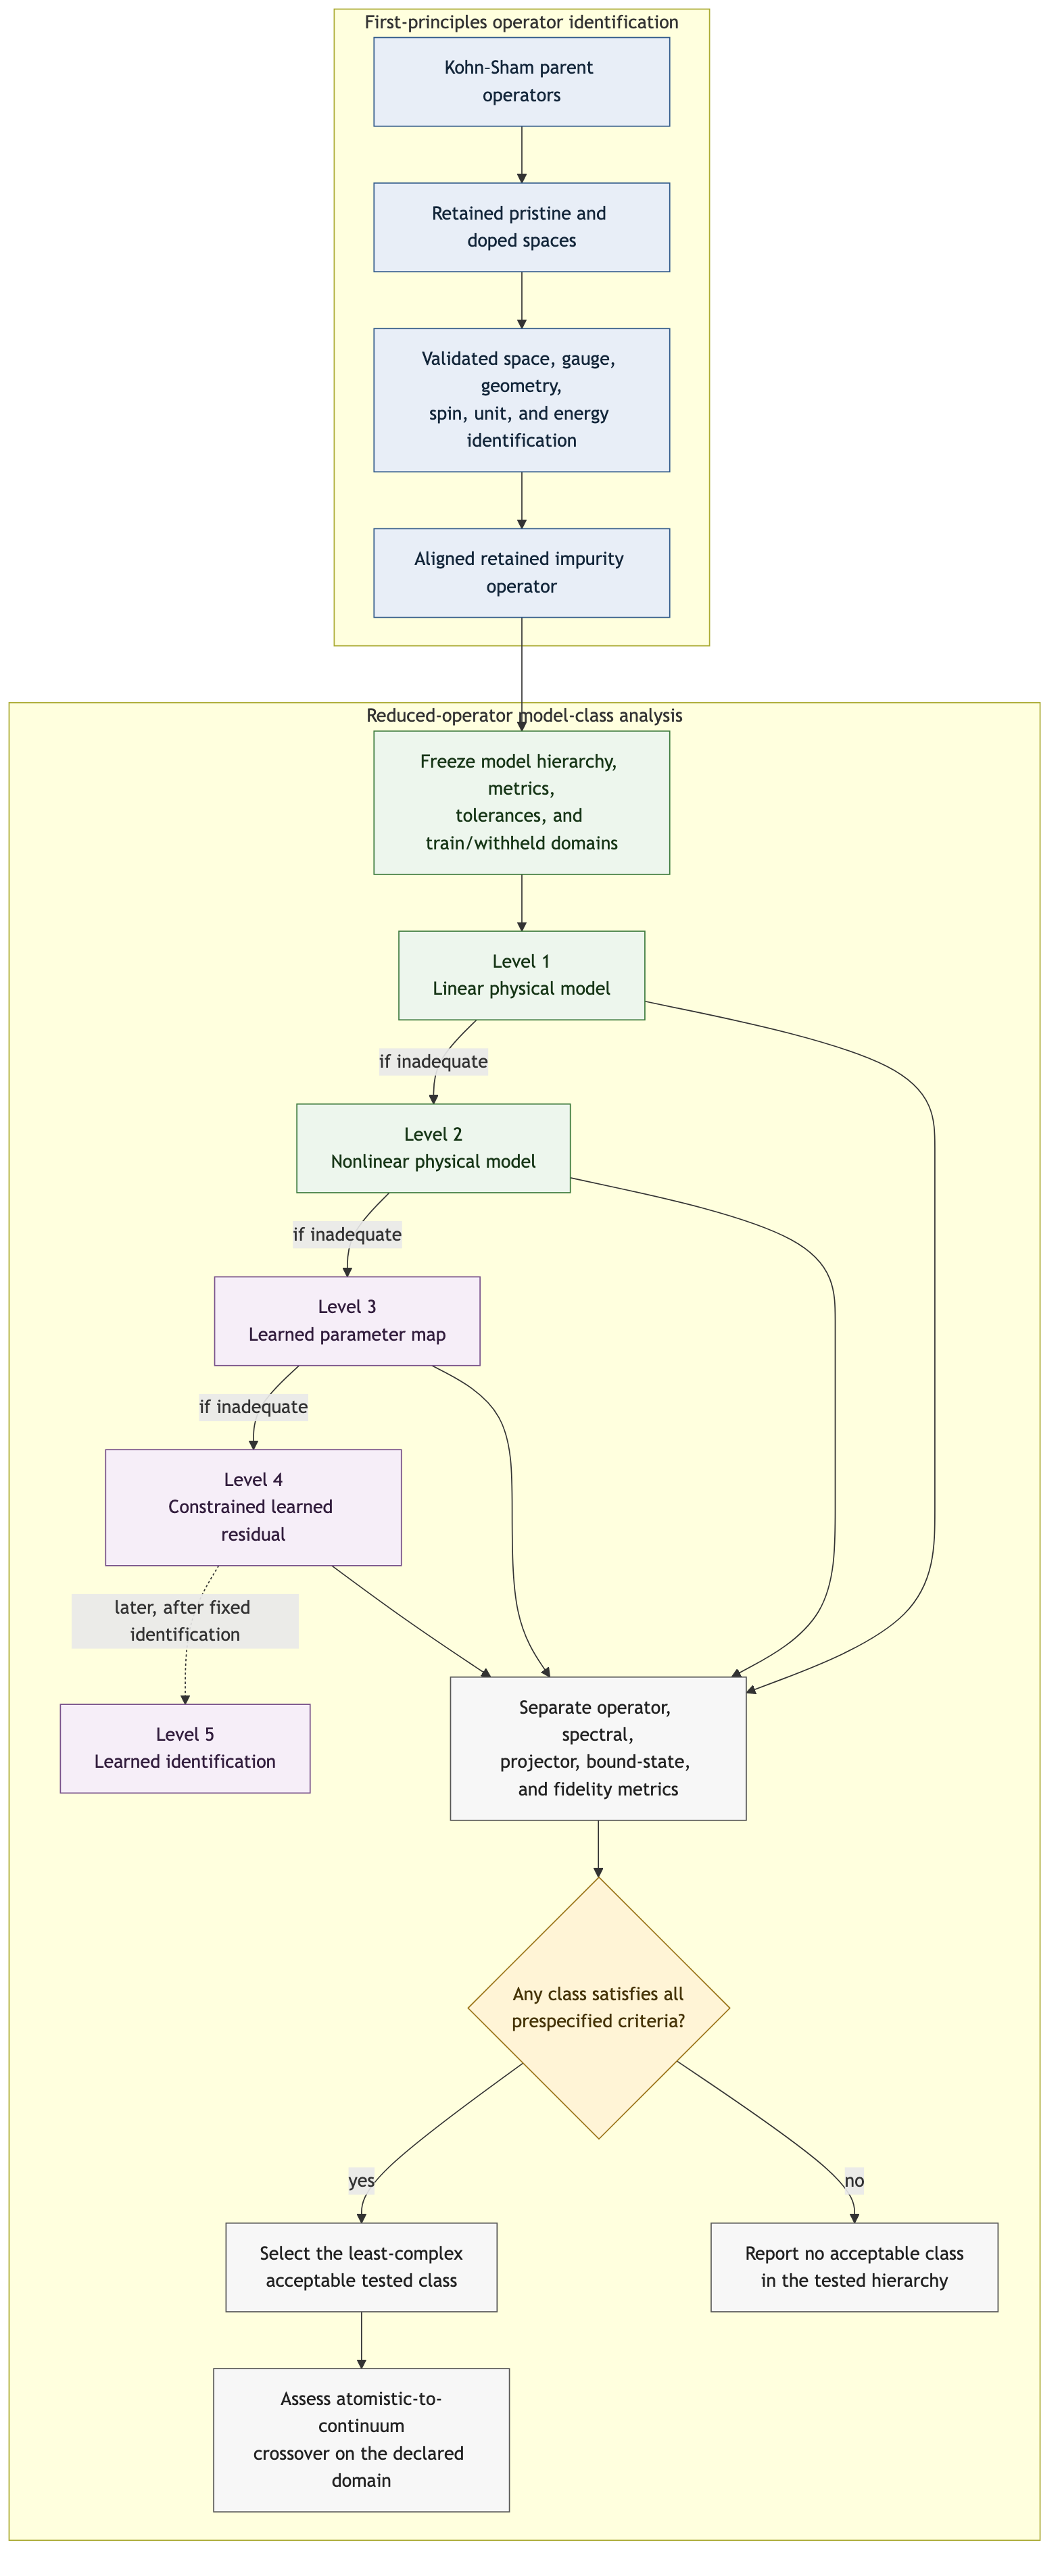
\includegraphics[
    width=\textwidth,
    height=0.80\textheight,
    keepaspectratio
  ]{figures/structured-learning-process.png}
  \caption{Proposed operator-identification and structured-learning process.
  Solid arrows show the fixed-identification progression and escalation through
  increasingly expressive model classes when a simpler tested class is
  inadequate. The dotted arrow marks learned identification as deferred work.
  The editable Mermaid source is retained in
  \texttt{figures/structured-learning-process.mmd}.}
  \label{fig:structured-learning-process}
\end{figure}

\section{A staged computational progression}

The proposed progression introduces flexibility only when a simpler level is
shown to be inadequate under its declared tests.

\begin{description}
  \item[Level 1: linear physical model.] Use fixed stencils or a linear
    Slater--Koster or tight-binding parameterization and solve by linear least
    squares when the model permits it.
  \item[Level 2: nonlinear differentiable physical model.] Retain a
    deterministic Hamiltonian constructor while optimizing nonlinear physical
    parameters.
  \item[Level 3: learned parameter map.] Introduce a neural map only when
    admissible parameters must depend nonlinearly on a declared local
    environment.
  \item[Level 4: learned residual operator.] Fit the constrained correction
    beyond simpler accepted physical classes and decompose the residual by
    physical operator content.
  \item[Level 5: learned identification.] Only after fixed-identification
    behavior is understood, investigate optimization over an admissible gauge
    or identification manifold.
\end{description}

Failure can be informative. Success at Level~1 would show that the tested target
requires no learned parameter map for the declared use. A gain at Level~2 would
show the value of nonlinear parameter dependence within the same constructor.
A reproducible gain from a structured learned model would identify missing
expressiveness in the simpler tested classes. Failure of an expressive model
under fixed constraints may indicate incompatible constraints, inadequate
descriptors, insufficient data, or optimization failure; these alternatives
must be distinguished before a scientific interpretation is assigned.

\section{Scientific question and evidence boundary}

The proposed central question is
\begin{quote}
What is the lowest-complexity operator class in which the aligned retained
Kohn--Sham impurity problem is representable within prespecified tolerances for
a declared use?
\end{quote}
For each candidate class $\mathfrak M$, let $\mathfrak A_{\mathfrak M}$ be the
subset satisfying every prespecified operator, spectral, projector, bound-state,
fidelity, and exact structural criterion applicable to the declared use. One
formal expression is
\begin{equation}
  \mathfrak M^{\ast}
  \in
  \arg\min_{\substack{\mathfrak M\in\mathfrak H\\
                      \mathfrak A_{\mathfrak M}\ne\varnothing}}
  \operatorname{complexity}(\mathfrak M).
  \label{eq:minimal-operator-class}
\end{equation}
The condition $\epsilon(\mathfrak M)\leq\epsilon_{\rm target}$ may define the
operator-error component of $\mathfrak A_{\mathfrak M}$, but it cannot replace
the other required criteria. The candidate hierarchy $\mathfrak H$, complexity
ordering, metrics, tolerances, training protocol, and withheld validation domain
are frozen before selection. If no tested class passes, no acceptable class has
been identified within the tested hierarchy.

A constrained neural model is thus an expressive comparator, not the central
physical model and not an infallible oracle. It can help test whether a simpler
physical class has exhausted its representational capacity only when
optimization adequacy and generalization have independent evidence. The
complete proposed pipeline is the process shown in
Figure~\ref{fig:structured-learning-process}.

This framing makes the learning component useful because it is accountable to
the operator-identification framework. It asks not whether a flexible model can
fit a matrix, but which physically interpretable restrictions can be retained
without losing the parent information required for the intended reduction.

\include{chapters/07-verification-and-validation}
\include{chapters/08-results-and-limitations}
\include{chapters/09-conclusions-and-outlook}

\appendix
\chapter{Notation, Conventions, and Status Vocabulary}
\index{notation|textbf}
\index{convention|textbf}

\label{app:notation-and-status}

This appendix is an expository index for the monograph. It does not override the
applicable specifications, proof contracts, software schemas, or retained
evidence. A symbol used by an owning record retains the definition in that
record when it is more specific than the summary below.

\section{Physical and mathematical objects}
\index{physical model}
\index{mathematical operator}
\index{software artifact}


\begin{center}
\small
\begin{tabular}{@{}p{0.20\textwidth}p{0.70\textwidth}@{}}
\toprule
Symbol or term & Meaning in this monograph \\
\midrule
Physical model & A declared material and physical approximation, including its
state variables, branch, and intended interpretation. \\
$\widehat H$ & An abstract Hamiltonian operator on an identified state space;
not a finite matrix unless a representation has been selected. \\
$H$ & A finite matrix representation whose space, basis, geometry, units,
energy reference, spin convention, and gauge must be identified. \\
$\mathcal H$ & An ambient one-particle state space. \\
$\mathcal S$ & A finite retained subspace of an ambient state space. \\
$P_{\mathcal S}$ & Orthogonal projector from the ambient space onto
$\mathcal S$. \\
$\mathcal B$ & An ordered basis for a represented finite space. \\
$N$ or $M$ & A finite represented or retained dimension, as locally defined. \\
$\dagger$ & Adjoint or conjugate transpose in the stated finite-dimensional
inner-product setting. \\
\bottomrule
\end{tabular}
\end{center}

\section{Periodic and Wannier notation}
\index{notation!Bloch and Wannier}


\begin{center}
\small
\begin{tabular}{@{}p{0.20\textwidth}p{0.70\textwidth}@{}}
\toprule
Symbol & Meaning \\
\midrule
$\mathbf r$ & Real-space position coordinate. \\
$\mathbf k$ & Crystal momentum in a declared reciprocal-coordinate convention. \\
$\mathbf R$ & Bravais-lattice translation. \\
$\psi_{n\mathbf k}$ & Bloch state with local band or frame index $n$. \\
$u_{n\mathbf k}$ & Cell-periodic factor of a Bloch state. \\
$U(\mathbf k)$ & Momentum-dependent unitary frame choice within a retained
Bloch subspace; not to be confused with an interspace identification below. \\
$w_{n\mathbf R}$ & Wannier basis function generated from a retained Bloch frame. \\
$H^{(\mathrm W)}(\mathbf k)$ & Hamiltonian matrix in the selected Wannier
frame at $\mathbf k$. \\
$H^{(\mathrm W)}(\mathbf R)$ & Real-space Wannier Hamiltonian block under the
recorded Fourier convention. \\
$N_{\mathbf k}$ & Number of sampled wavevectors in the applicable uniform grid. \\
\bottomrule
\end{tabular}
\end{center}

The same letter $U$ is conventional for both a Wannier gauge and an interspace
identification. The local domain and codomain must disambiguate it. Where
confusion is likely, the monograph uses $G$ for an in-space gauge rotation and
$U$ or $A$ for a map between retained spaces.

\section{Frames, gauges, and alignment}
\index{notation!alignment}


\begin{center}
\small
\begin{tabular}{@{}p{0.20\textwidth}p{0.70\textwidth}@{}}
\toprule
Symbol & Meaning \\
\midrule
$V$ & Rectangular matrix whose orthonormal columns form a retained frame. \\
$G$ & Unitary coordinate change within one retained space. \\
$VV^{\dagger}$ & Ambient-space projector associated with an orthonormal frame. \\
$U$ or $A$ & Explicit identification between two retained spaces; its direction
is stated with its definition. \\
$H_b$ & Pristine or bulk represented Hamiltonian in its declared coordinates. \\
$H_d$ & Doped represented Hamiltonian for dopant $d$. \\
$G_b,G_d$ & Independent unitary coordinate changes in pristine and doped
retained spaces. \\
$\Delta H_{d\to b}$ & Doped operator pulled into pristine coordinates and then
subtracted: $U^{\dagger}H_dU-H_b$. \\
$\Delta H_{b\to d}$ & Pristine operator pushed into doped coordinates and then
subtracted: $H_d-UH_bU^{\dagger}$. \\
$\overline H$ & Operator after application of the explicitly recorded scalar
energy-reference convention. \\
$\theta_j$ & Principal angle between two retained subspaces. \\
\bottomrule
\end{tabular}
\end{center}

A subscript $b$ denotes bulk or pristine material, while $d$ denotes a dopant
branch. When the identity of the dopant matters,
$d\in\{\mathrm P,\mathrm B\}$. Neither notation fixes charge state, spin branch,
or supercell size without an accompanying record.

\section{Reduction notation}

\begin{center}
\small
\begin{tabular}{@{}p{0.20\textwidth}p{0.70\textwidth}@{}}
\toprule
Symbol & Meaning \\
\midrule
$\mathfrak M_j$ & Declared reduced-model class indexed by complexity or another
frozen ordering. \\
$\boldsymbol\theta$ & Parameter vector within a declared model class. \\
$f_{\phi}$ & Learned parameter map with trainable parameters $\phi$ and declared
physical descriptors as inputs. \\
$\mathcal C$ & Deterministic constructor mapping admissible parameters to a
represented Hamiltonian. \\
$\epsilon(\mathfrak M)$ & Best declared normalized discrepancy attainable in
model class $\mathfrak M$; a computed fit need not attain this infimum. \\
$\mathcal L_E$ & Spectral training objective with stated data, weights, units,
and normalization. \\
$\mathcal L_H$ & Aligned represented-operator objective. \\
$\tau_E,\tau_H$ & Prespecified spectral and operator tolerances. \\
$\mathfrak A_{E,j}$ & Spectral-admissible subset of model class $j$. \\
$\mathfrak A_{H,j}$ & Operator-admissible subset of model class $j$. \\
$d_{\mathrm{TB}}$ & Declared metric on compatible canonical tight-binding
coordinates. \\
$\delta_j^{\ast}$ & Minimum or infimum separation between the two admissible
sets, according to the established assumptions. \\
$\mathcal R$ & Reduction map with an explicitly stated domain and codomain. \\
$\varepsilon_{\mathrm{path}}$ & Norm of the difference between two aligned
reduction paths. \\
\bottomrule
\end{tabular}
\end{center}

The words \emph{projection}, \emph{disentanglement}, \emph{basis
transformation}, \emph{localization}, \emph{truncation}, \emph{fitting}, and
\emph{reduction} denote different operations. They are not used as synonyms.

\section{Excluded-space and continuum notation}

\begin{center}
\small
\begin{tabular}{@{}p{0.20\textwidth}p{0.70\textwidth}@{}}
\toprule
Symbol & Meaning \\
\midrule
$P,Q$ & Complementary orthogonal projectors with $P+Q=I$. A superscript $(P)$
marks restriction to the retained $P$ space; phosphorus is written $\mathrm P$
when ambiguity is possible. \\
$H_{PP},H_{PQ}$ & Blocks such as $PHP$ and $PHQ$ in a declared decomposition. \\
$H_{\mathrm{eff}}(E)$ & Energy-dependent Feshbach effective operator in the
retained $P$ space. \\
$\Delta_Q$ & Distance from $E$ to the spectrum of $H_{QQ}$ in the declared
self-adjoint resolvent setting. \\
$V_{\mathrm{cont},d}$ & Candidate continuum impurity operator for dopant $d$. \\
$D_d$ & Aligned atomistic-minus-continuum discrepancy. \\
$P_{>R}$ & Projector onto a declared exterior region beyond radius $R$. \\
$\eta_d(R)$ & Exterior residual $\|P_{>R}D_dP_{>R}\|$ in a declared norm. \\
$r_{c,d}(\tau)$ & Tolerance-dependent crossover infimum; not a universal
material constant. \\
$J$ & Continuum-to-atomistic or continuum-to-Wannier embedding, with its
normalization and validation domain stated separately. \\
\bottomrule
\end{tabular}
\end{center}

\citationtodo{low priority}{Check the naming and definition of the
energy-dependent Feshbach effective operator against Feshbach (1958),
bibliography key \texttt{feshbach1958} (already present).}

\section{Norms and residuals}
\index{norm}
\index{residual}


\begin{align}
  \|A\|_{\mathrm F}
  &=
  \left(\sum_{i,j}|A_{ij}|^2\right)^{1/2},\\
  \|A\|_2
  &=
  \sup_{x\ne0}\frac{\|Ax\|_2}{\|x\|_2},\\
  \|A\|_{\max}
  &=
  \max_{i,j}|A_{ij}|.
\end{align}

The Frobenius and induced Euclidean operator norms are invariant under unitary
conjugation. Entrywise maxima, shell decompositions, and spatial truncations may
have narrower invariance groups. Every reported residual states whether it is
absolute or normalized and gives its units and zero-scale behavior.

\section{Proof status}

\begin{description}
  \item[\texttt{proposed}.] Statement, definitions, or strategy exists without a
    complete established proof.
  \item[\texttt{in development}.] Proof construction is active and immediate
    prerequisites are sufficiently identified.
  \item[\texttt{blocked}.] A named missing assumption, definition, prerequisite,
    or human scientific decision prevents progress.
  \item[\texttt{complete, unreviewed}.] A complete derivation is recorded but
    has not passed independent mathematical review.
  \item[\texttt{reviewed}.] The derivation and declared prerequisites passed
    independent mathematical review.
  \item[\texttt{numerically checked}.] Separate numerical evidence agrees under
    declared conditions; this supplements rather than replaces proof.
  \item[\texttt{retired}.] The claim was superseded, merged, or rejected with a
    recorded disposition.
\end{description}

A mechanization contract may separately be \texttt{frozen}, \texttt{encoded},
\texttt{checked}, or \texttt{cross-checked} in each backend. These words do not
replace the proof-package status. In particular, the currently checked Lean
encoding of \texttt{PRF-05.01} does not make the entire \texttt{PRF-05} package
complete or reviewed.

\section{Scientific and evidentiary status}
\index{evidence!status vocabulary}


\begin{description}
  \item[Calculated result.] Produced by an identified calculation with retained
    provenance.
  \item[Literature value.] Taken from an identified and verified source.
  \item[Expected behavior.] A prediction, not an observation.
  \item[Illustrative example.] Explanatory material without research-evidence
    status.
  \item[Synthetic test data.] Constructed for software or numerical testing.
  \item[Placeholder.] Incomplete material awaiting authoritative content.
  \item[Proposed work.] Planned but not completed.
\end{description}

Mathematical proof, software verification, numerical verification, scientific
validation, and uncertainty quantification remain distinct evidence types. A
claim may require more than one of them, and none is inferred merely from the
presence of the others.

\section{Units and coordinate conventions}
\index{units}
\index{coordinate convention}


Every physical numerical value states its unit. Energy references used for
plots, bulk observables, and pristine--doped subtraction are identified
separately. Real-space coordinates identify lattice vectors, cell convention,
and site mapping. Reciprocal coordinates identify the reciprocal basis and any
path parameterization. Spinless, collinear-spin, and noncollinear spinor
representations are never mixed implicitly.

The notation in this appendix is intentionally insufficient to authorize a
comparison. The represented records and owning specifications must still supply
the exact metadata needed by the operation.

\chapter{Hilbert--Schmidt Geometry and the Frobenius Norm}
\label{app:hilbert-schmidt-and-frobenius}

\textbf{Status: expository appendix.} This appendix records the operator-space geometry
underlying Frobenius-norm comparisons of reduced operators. It does not define
a scientific acceptance metric.

\section{Hilbert--Schmidt inner product}

Let $V$ be a finite-dimensional complex Hilbert space, and let
$\mathcal L(V)$ denote the vector space of linear operators from $V$ to itself.
If $\dim V=d$, then $\dim\mathcal L(V)=d^2$. The function
\begin{equation}
    \langle\cdot,\cdot\rangle_{\mathrm{HS}}:
    \mathcal L(V)\times\mathcal L(V)
    \longrightarrow
    \mathbb C
\end{equation}
defined by
\begin{equation}
    \langle A,B\rangle_{\mathrm{HS}}
    =
    \operatorname{Tr}\!\left(A^\dagger B\right)
\end{equation}
is the \emph{Hilbert--Schmidt inner product}, also called the trace inner
product~\cite{nielsenchuang2010}. With this convention it is conjugate-linear
in its first argument and linear in its second. Its induced norm is
\begin{equation}
    \lVert A\rVert_{\mathrm{HS}}
    =
    \sqrt{
        \operatorname{Tr}\!\left(A^\dagger A\right)
    }.
\end{equation}

Let $\mathcal H^{(P)}$ be a finite-dimensional retained Hilbert space. The
operator space
\begin{equation}
    \mathcal L\!\left(\mathcal H^{(P)}\right)
\end{equation}
is itself a finite-dimensional Hilbert space under this inner product. If
\begin{equation}
    \hat A,\hat B:
    \mathcal H^{(P)}
    \longrightarrow
    \mathcal H^{(P)},
\end{equation}
then their sum and difference are well-defined elements of the same operator
space:
\begin{equation}
    \hat A\pm\hat B:
    \mathcal H^{(P)}
    \longrightarrow
    \mathcal H^{(P)}.
\end{equation}

Given an orthonormal basis of $\mathcal H^{(P)}$, let $\mathbf A$ and
$\mathbf B$ be the matrices representing $\hat A$ and $\hat B$. The
Hilbert--Schmidt inner product becomes the Frobenius inner product,
\begin{equation}
    \langle\mathbf A,\mathbf B\rangle_{\mathrm F}
    =
    \operatorname{Tr}\!\left(\mathbf A^\dagger\mathbf B\right),
\end{equation}
and the corresponding norm satisfies
\begin{equation}
    \lVert\mathbf A\rVert_{\mathrm F}^2
    =
    \operatorname{Tr}\!\left(\mathbf A^\dagger\mathbf A\right)
    =
    \sum_{i,j}\lvert A_{ij}\rvert^2.
\end{equation}
Thus the Frobenius norm is the matrix-coordinate form of the
Hilbert--Schmidt norm when the coordinates are defined by an orthonormal basis.

Operators may be added and subtracted because they belong to a common operator
vector space. The legitimacy of an operator subtraction does not follow merely
from two matrices having the same dimensions. It follows from the represented
operators having compatible domains and codomains and from the matrices using
an identified common state space and basis convention.

\section{Common projection and reduced components}

Let $\hat P$ be an orthogonal projector and define
\begin{equation}
    \mathcal H^{(P)}
    =
    \operatorname{Ran}\hat P.
\end{equation}
For possibly unbounded parent operators $\hat H$ and $\hat T$, assume that the
retained range lies in the domains needed to define the compressions below.
Set
\begin{align}
    \hat H_{\mathrm{eff}}
    &=
    \left.
        \hat P\hat H\hat P
    \right|_{\mathcal H^{(P)}},
    \\
    \hat T_{\mathrm{eff}}
    &=
    \left.
        \hat P\hat T\hat P
    \right|_{\mathcal H^{(P)}}.
\end{align}
Both reduced operators belong to
$\mathcal L\!\left(\mathcal H^{(P)}\right)$. Their difference is therefore a
well-defined reduced operator,
\begin{equation}
    \hat V_{\mathrm{eff}}
    =
    \hat H_{\mathrm{eff}}
    -
    \hat T_{\mathrm{eff}},
\end{equation}
and, by construction,
\begin{equation}
    \hat H_{\mathrm{eff}}
    =
    \hat T_{\mathrm{eff}}
    +
    \hat V_{\mathrm{eff}}.
\end{equation}

If the parent operators satisfy
$\hat H=\hat T+\hat V$ on a compatible domain, linearity gives
\begin{equation}
    \hat V_{\mathrm{eff}}
    =
    \left.
        \hat P\hat V\hat P
    \right|_{\mathcal H^{(P)}}.
\end{equation}
Even when $\hat V$ is a local multiplication operator in the parent position
representation, its compression need not act as multiplication by a scalar
function within the retained representation. Projection can produce an
operator that is nonlocal in the retained coordinates. If the parent
Hamiltonian contains nonlocal pseudopotential, spin--orbit, or other operator
components, the chosen kinetic--remainder decomposition must identify those
components explicitly.

\section{Aligned pristine--doped operators}

The same common-space requirement applies to independently constructed
pristine and doped retained operators. Suppose first that the two retained
spaces have equal finite dimension and that a physically admissible unitary
identification has been constructed,
\begin{equation}
    \hat U_d:
    \mathcal H_b^{(P)}
    \longrightarrow
    \mathcal H_d^{(P)}.
\end{equation}
Let $c_b$ and $c_d$ denote scalar energy references selected by the declared
alignment procedure, and define
\begin{equation}
    \overline{\hat H}_s^{(P)}
    =
    \hat H_s^{(P)}-c_s\hat I_s,
    \qquad
    s\in\{b,d\}.
\end{equation}
The aligned impurity operator on the bulk retained space is then
\begin{equation}
    \Delta\hat H_d^{(P)}
    =
    \hat U_d^\dagger
    \overline{\hat H}_d^{(P)}
    \hat U_d
    -
    \overline{\hat H}_b^{(P)}
    \in
    \mathcal L\!\left(\mathcal H_b^{(P)}\right).
\end{equation}
Equal matrix dimensions alone would not establish this membership. The
identification must also preserve the physical structures required by the
comparison, including the applicable gauge, geometry, orbital ordering, spin
structure, and energy reference.

The Hilbert--Schmidt discrepancy of the aligned operator is
\begin{equation}
    \left\lVert
        \Delta\hat H_d^{(P)}
    \right\rVert_{\mathrm{HS}}^2
    =
    \operatorname{Tr}\!\left[
        \left(\Delta\hat H_d^{(P)}\right)^\dagger
        \Delta\hat H_d^{(P)}
    \right].
\end{equation}
In a common orthonormal numerical basis, this is exactly
\begin{equation}
    \left\lVert
        \Delta\mathbf H_d^{(P)}
    \right\rVert_{\mathrm F}^2
    =
    \sum_{\alpha,\beta}
    \left\lvert
        \Delta H_{d,\alpha\beta}^{(P)}
    \right\rvert^2.
\end{equation}
Frobenius-norm minimization is therefore least-squares approximation in the
finite-dimensional Hilbert space of retained operators.

\section{Domains and the particle in a box}

The differential expression
\begin{equation}
    -\frac{\hbar^2}{2m}\frac{d^2}{dx^2}
\end{equation}
does not by itself specify a quantum-mechanical operator. An operator is
determined by both its action and its domain. The free kinetic operator on the
real line and the kinetic operator on a finite interval with Dirichlet boundary
conditions are therefore different operators even though they share the same
differential expression.

For the particle in a box, let
\begin{equation}
    \hat H_{\mathrm{box}}
    =
    -\frac{\hbar^2}{2m}\frac{d^2}{dx^2},
    \qquad
    \mathcal D(\hat H_{\mathrm{box}})
    =
    H^2(0,L)\cap H_0^1(0,L).
\end{equation}
If $\hat T$ is this same Dirichlet kinetic operator, then
$\hat H_{\mathrm{box}}=\hat T$ and consistent projection gives
\begin{equation}
    \hat H_{\mathrm{eff}}-\hat T_{\mathrm{eff}}
    =
    \hat 0.
\end{equation}

A nonzero difference can arise if the chosen reference kinetic operator does
not carry the same confinement or boundary-domain structure. Such a comparison
first requires an explicit common-space identification. The resulting residual
can then record the missing confinement or boundary contribution relative to
the chosen reference kinetic operator; it must not be identified automatically
with a local physical potential. This distinction separates a mathematically
valid represented subtraction from its physical interpretation.

\section{Infinite-dimensional qualification}

For an infinite-dimensional Hilbert space $\mathcal H$, the space of all
bounded linear operators is not a Hilbert space under the Hilbert--Schmidt inner
product. One instead uses the Hilbert--Schmidt class
\begin{equation}
    \mathcal L_2(\mathcal H)
    =
    \left\{
        \hat A:
        \operatorname{Tr}\!\left(\hat A^\dagger\hat A\right)
        <
        \infty
    \right\}.
\end{equation}
For $\hat A\in\mathcal L_2(\mathcal H)$,
\begin{equation}
    \lVert\hat A\rVert_{\mathrm{HS}}^2
    =
    \operatorname{Tr}\!\left(\hat A^\dagger\hat A\right).
\end{equation}
Finite-rank operators are Hilbert--Schmidt. Consequently, a well-defined
compression to a finite-dimensional retained space has finite
Hilbert--Schmidt norm.

The Frobenius norm is invariant under a common unitary change of orthonormal
coordinates:
\begin{equation}
    \left\lVert
        \mathbf U^\dagger\mathbf A\mathbf U
        -
        \mathbf U^\dagger\mathbf B\mathbf U
    \right\rVert_{\mathrm F}
    =
    \lVert\mathbf A-\mathbf B\rVert_{\mathrm F}.
\end{equation}
It is not meaningful to invoke this invariance when only one operand has been
transformed or when the two matrices have not first been placed in a common
represented space.

The Hilbert--Schmidt geometry supplies a rigorous finite-dimensional setting
for operator comparison and Frobenius-norm minimization. It does not by itself
make the Frobenius norm the scientifically appropriate loss. The common state
space, retained subspace, normalization, alignment, weighting, domains, energy
reference, and relation of the norm to the observables of interest must still
be specified.


\part*{Notes}
\addcontentsline{toc}{part}{Notes}
\markboth{Notes}{Notes}

The notes collect supporting derivations and conceptual clarifications that are
useful to the monograph but remain distinct from its main chapter sequence.
Their inclusion does not elevate illustrative material or proposed metrics to
research evidence.

\notechapter{1}{Operator spaces, compression, and alignment}

\section*{Scope}

The replacement of a first-principles Hamiltonian by a finite model is not
defined solely by retaining a selected set of eigenvalues. A reduced
description must specify the state space on which the reduced operator acts,
the map from the parent space to that state space, the coordinate
representation used for its matrix elements, and the class of operators
admitted as candidate models. These choices determine which algebraic
operations are meaningful and which physical interpretations can be assigned
to their results.

The distinction is particularly important when the parent Hamiltonian is an
unbounded differential operator, while the reduced description is a finite
matrix. In the continuum, the operator domain and boundary conditions are part
of the Hamiltonian. In the retained representation, those data are no longer
written as an explicit domain, but their consequences remain encoded in the
matrix. A rigorous reduction must therefore distinguish the continuum
operator, the retained operator, and the numerical matrix representing that
operator.

\section*{Operators and their domains}

Let $\mathcal H$ be a complex Hilbert space. An unbounded operator is a map
\begin{equation}
    \hat A:
    \mathcal D(\hat A)\subseteq\mathcal H
    \longrightarrow
    \mathcal H,
\end{equation}
where the domain $\mathcal D(\hat A)$ is part of the definition of $\hat A$.
Two operators may have the same formal differential action and nevertheless
define different physical systems because they act on different domains. For
quantum Hamiltonians, the distinction between a symmetric differential
expression and a self-adjoint operator is essential: self-adjointness requires
equality of both the operator action and the adjoint domain~\cite{teschl2014,reedSimon1975,schmudgen2012}.

The sum or difference of two unbounded operators is initially defined on the
intersection of their domains,
\begin{equation}
    \mathcal D(\hat A\pm\hat B)
    =
    \mathcal D(\hat A)\cap\mathcal D(\hat B).
\end{equation}
Consequently, an expression such as
\begin{equation}
    \hat V=\hat H-\hat T
\end{equation}
is an operator identity only after the operators and their compatible domains
have been specified. This qualification is not an objection to subtraction.
It identifies the mathematical data required for the subtraction to refer to
a common operator space.

\section*{Spectral restriction}

Consider a self-adjoint Hamiltonian $\hat H$ with a pure-point spectral sector,
\begin{equation}
    \hat H\lvert\psi_i\rangle
    =
    E_i\lvert\psi_i\rangle,
\end{equation}
where the retained eigenvectors are orthonormal. Let $\mathcal I_P$ denote the
selected set of spectral indices and define
\begin{equation}
    \hat P
    =
    \sum_{i\in\mathcal I_P}
    \lvert\psi_i\rangle\langle\psi_i\rvert,
\end{equation}
with retained space
\begin{equation}
    \mathcal H^{(P)}
    =
    \operatorname{Ran}\hat P.
\end{equation}
If an energy cutoff intersects a degenerate eigenspace, the full degenerate
eigenspace must be retained if the construction is to remain invariant under
unitary rotations within that eigenspace. More generally, the selected range
should be an invariant subspace of the parent operator.

The retained Hamiltonian is
\begin{equation}
    \hat H^{(P)}
    =
    \left.
        \hat P\hat H\hat P
    \right|_{\mathcal H^{(P)}}:
    \mathcal H^{(P)}
    \longrightarrow
    \mathcal H^{(P)}.
\end{equation}
It reproduces the action of the parent Hamiltonian exactly on the selected
invariant subspace. When $\hat P\hat H\hat P$ is instead regarded as an
operator on the full parent space, it acts as zero on
$\operatorname{Ran}(\hat I-\hat P)$. That zero action is an embedding
convention; it is not the parent Hamiltonian on the discarded sector.

This distinction separates three objects:
\begin{equation}
    \hat H,
    \qquad
    \hat H^{(P)},
    \qquad
    \mathbf H^{(P)}.
\end{equation}
They denote, respectively, the parent operator, the retained operator, and a
matrix representation of the retained operator in a declared basis. Treating
them as interchangeable obscures the state-space maps on which later
comparisons depend.

\section*{Compression and downfolding}

A fixed-subspace compression should not be identified with an effective
Hamiltonian obtained by eliminating the complementary sector. With
\begin{equation}
    \hat Q=\hat I-\hat P,
\end{equation}
a Feshbach--L\"owdin construction gives the energy-dependent operator
\begin{equation}
    \hat H_{\mathrm{down}}(E)
    =
    \hat P\hat H\hat P
    +
    \hat P\hat H\hat Q
    \left(E-\hat Q\hat H\hat Q\right)^{-1}
    \hat Q\hat H\hat P,
\end{equation}
whenever the reduced resolvent exists~\cite{lowdin1982}. The second term
represents virtual excursions into the eliminated subspace. In general,
\begin{equation}
    \hat H_{\mathrm{down}}(E)
    \neq
    \hat H^{(P)}.
\end{equation}
The approximation target must therefore be declared explicitly. A model
fitted to $\hat H^{(P)}$ approximates the parent action on a selected subspace.
A model fitted to $\hat H_{\mathrm{down}}(E)$ also attempts to reproduce
eliminated-space effects and may inherit energy dependence and nonlocality.

\section*{Common compression and additive structure}

Suppose that
\begin{equation}
    \hat H=\hat T+\hat V
\end{equation}
is valid on a compatible domain, and assume that the finite-dimensional
retained space lies within the required domains. Applying the same compression
to every term gives
\begin{equation}
    \hat H^{(P)}
    =
    \hat T^{(P)}+\hat V^{(P)},
\end{equation}
where
\begin{equation}
    \hat T^{(P)}
    =
    \left.\hat P\hat T\hat P\right|_{\mathcal H^{(P)}},
    \qquad
    \hat V^{(P)}
    =
    \left.\hat P\hat V\hat P\right|_{\mathcal H^{(P)}}.
\end{equation}
It follows that
\begin{equation}
    \hat V^{(P)}
    =
    \hat H^{(P)}-\hat T^{(P)}.
\end{equation}
The subtraction is valid because the corresponding addition was performed in
the common vector space
\begin{equation}
    \mathcal L\!\left(\mathcal H^{(P)}\right).
\end{equation}

The physical interpretation of the difference is a separate question.
Although $\hat V$ may be a local multiplication operator in the parent
position representation, $\hat P\hat V\hat P$ is generally nonlocal. If
\begin{equation}
    \langle x\rvert\hat V\lvert x'\rangle
    =
    V(x)\delta(x-x'),
\end{equation}
then
\begin{equation}
    V^{(P)}(x,x')
    =
    \int dy\,
    P(x,y)V(y)P(y,x'),
\end{equation}
which is not generally proportional to $\delta(x-x')$. Locality must therefore
be treated as an admissible model assumption rather than as an automatic
consequence of projection.

\section*{Hilbert--Schmidt geometry}

The space of all bounded operators on an infinite-dimensional Hilbert space is
not a Hilbert space under the trace inner product. The relevant
infinite-dimensional space is the Hilbert--Schmidt class
\begin{equation}
    \mathfrak S_2(\mathcal H)
    =
    \left\{
        \hat A\in\mathcal B(\mathcal H)
        \;\middle|\;
        \operatorname{Tr}(\hat A^\dagger\hat A)<\infty
    \right\},
\end{equation}
with
\begin{equation}
    \langle\hat A,\hat B\rangle_{\mathrm{HS}}
    =
    \operatorname{Tr}(\hat A^\dagger\hat B)
\end{equation}
and
\begin{equation}
    \lVert\hat A\rVert_{\mathrm{HS}}^2
    =
    \operatorname{Tr}(\hat A^\dagger\hat A)
\end{equation}
\cite{simon2005}. Full continuum Hamiltonians are generally unbounded and are
not Hilbert--Schmidt operators. The trace inner product should not be applied
to them without an additional construction.

Finite-dimensional retained operators avoid this obstruction. In any
orthonormal basis of an $M$-dimensional retained space,
\begin{equation}
    \lVert\hat A\rVert_{\mathrm{HS}}^2
    =
    \sum_{\alpha,\beta=1}^{M}
    \lvert A_{\alpha\beta}\rvert^2
    =
    \lVert\mathbf A\rVert_{\mathrm F}^2.
\end{equation}
The Frobenius norm is therefore the coordinate representation of the
Hilbert--Schmidt norm. Its unitary invariance makes it suitable for operator
comparisons after the relevant state spaces have been identified. It does not
determine the identification itself.

\section*{Alignment across retained spaces}

Let $\hat H_b^{(P)}$ and $\hat H_d^{(P)}$ denote retained pristine and doped
Hamiltonians acting on $\mathcal H_b^{(P)}$ and $\mathcal H_d^{(P)}$. Equal
matrix dimensions do not imply that the two matrices represent operators on
the same physical state space. A unitary identification
\begin{equation}
    \hat U_d:
    \mathcal H_b^{(P)}
    \longrightarrow
    \mathcal H_d^{(P)}
\end{equation}
must first be specified. The aligned difference is
\begin{equation}
    \Delta\hat H_d^{(P)}
    =
    \hat U_d^\dagger
    \hat H_d^{(P)}
    \hat U_d
    -
    \hat H_b^{(P)}.
\end{equation}

Wannier functions provide localized frames for such comparisons, but their
construction includes unitary gauge freedom, and an entangled band manifold
requires an explicit retained-subspace selection~\cite{marzari2012,souza2001}.
The alignment record must therefore include the retained subspaces, orbital
labels, gauge, geometry, units, spin convention, and energy reference.

The fundamental conclusion is that model reduction is performed on identified
operator spaces, not on arrays whose dimensions happen to agree. Once the
spaces and maps are fixed, subtraction and Hilbert--Schmidt comparison are
mathematically straightforward. The scientific content lies in justifying the
projection, the identification, and the admissible model class.

\input{notes/particle-in-a-box-residuals}
\notechapter{3}{Preliminary Frobenius comparison of two quantum harmonic-oscillator constructions}

\textbf{Status: proposed preliminary experiment.} The comparison, convergence
study, and plots described in this note have not yet been carried out. No
numerical values or observations are reported. The purpose of the experiment is
to compare a ladder-operator representation with a harmonic-oscillator
potential enclosed by a finite Dirichlet box after both have been placed in the
same retained ladder coordinates.

\section*{Question addressed by the experiment}

The one-dimensional quantum harmonic oscillator admits the exact
ladder-operator representation
\begin{equation}
    \hat H_{\mathrm{QHO}}
    =
    \hbar\omega
    \left(
        \hat a^\dagger\hat a+\frac{1}{2}\hat I
    \right)
\end{equation}
on $L^2(\mathbb R)$. The same potential can be placed inside a particle in a
box and represented on a finite spatial grid. Enlarging the box is expected to
reduce the influence of the Dirichlet walls on low-lying oscillator states,
while refining the grid is expected to reduce spatial-discretization error.

The central quantity is not a raw difference between a ladder matrix and a grid
matrix. Those matrices act in different coordinate spaces and may have
different dimensions. Instead, the finite-box Hamiltonian must first be pulled
back to a declared finite ladder space. The primary question is then
\begin{quote}
How does the Frobenius discrepancy between the pulled-back finite-box operator
and the exact retained ladder Hamiltonian behave as the box is enlarged and the
spatial discretization is refined?
\end{quote}

This construction also permits comparisons between spatial discretization
schemes with different grid spacings or dimensions because every represented
operator is mapped to the same retained ladder coordinates before subtraction.

\section*{Exact retained ladder Hamiltonian}

The oscillator length is
\begin{equation}
    \ell
    =
    \sqrt{\frac{\hbar}{m\omega}}.
\end{equation}
The normalized number states satisfy
\begin{align}
    \hat a\lvert n\rangle
    &=
    \sqrt{n}\,\lvert n-1\rangle,
    \\
    \hat a^\dagger\lvert n\rangle
    &=
    \sqrt{n+1}\,\lvert n+1\rangle,
\end{align}
and
\begin{equation}
    \hat H_{\mathrm{QHO}}\lvert n\rangle
    =
    E_n\lvert n\rangle,
    \qquad
    E_n
    =
    \hbar\omega
    \left(n+\frac{1}{2}\right).
\end{equation}

For a retained dimension $K$, define the abstract comparison space
\begin{equation}
    \mathcal K_K
    =
    \operatorname{span}
    \left\{
        \lvert 0\rangle,\ldots,\lvert K-1\rangle
    \right\}.
\end{equation}
In the ordered number-state basis, the exact retained Hamiltonian is
\begin{equation}
    \mathbf H_{\mathrm{lad}}^{(K)}
    =
    \hbar\omega\,
    \operatorname{diag}
    \left(
        \frac{1}{2},
        \frac{3}{2},
        \ldots,
        K-\frac{1}{2}
    \right).
\end{equation}
This is an exact spectral restriction of the real-line oscillator. It is the
reference operator for the proposed Frobenius comparison.

A finite ladder representation has an algebraic truncation boundary. If
$\mathbf a_K$ is the compressed annihilation operator, then
\begin{equation}
    [\mathbf a_K,\mathbf a_K^\dagger]
    =
    \mathbf I_K
    -
    K\lvert K-1\rangle\langle K-1\rvert.
\end{equation}
This top-state defect should be recorded when ladder operators themselves are
compared, although it does not alter the diagonal reference energies written
above.

\section*{Harmonic potential inside a Dirichlet box}

Let $X>0$ be the box half-width. The finite-box continuum Hamiltonian is
\begin{equation}
    \hat H_X
    =
    -\frac{\hbar^2}{2m}\frac{d^2}{dx^2}
    +
    \frac{1}{2}m\omega^2x^2
\end{equation}
on $L^2((-X,X))$, with domain
\begin{equation}
    \mathcal D(\hat H_X)
    =
    H^2((-X,X))\cap H_0^1((-X,X)).
\end{equation}
Thus
\begin{equation}
    \psi(-X)=\psi(X)=0.
\end{equation}
For finite $X$, this is a different continuum operator from the oscillator on
$\mathbb R$. The difference is a boundary-domain effect, not a change to the
interior multiplication potential.

For a spatial representation labeled by $h$, let the numerical state space be
$\mathcal V_{X,h}$ and let
\begin{equation}
    \mathbf H_{X,h}
    =
    \mathbf T_{\mathrm D,X,h}
    +
    \mathbf V_{\mathrm{QHO},X,h}
    \in
    \mathcal L(\mathcal V_{X,h}).
\end{equation}
Here $\mathbf T_{\mathrm D,X,h}$ represents the kinetic operator with the
declared Dirichlet closure, and $\mathbf V_{\mathrm{QHO},X,h}$ represents the
interior potential $m\omega^2x^2/2$. For a uniform grid with $N$ interior
points,
\begin{equation}
    x_j=-X+j\Delta x,
    \qquad
    \Delta x=\frac{2X}{N+1},
    \qquad
    j=1,\ldots,N.
\end{equation}
The comparison below does not require two spatial representations to have the
same $N$ or $\Delta x$.

\section*{Map from ladder states to a spatial representation}

Let
\begin{equation}
    \psi_n(x)=\langle x\mid n\rangle
\end{equation}
be the normalized real-line oscillator eigenfunction. For a uniform grid,
define the quadrature-scaled sampled vector
\begin{equation}
    \mathbf s_{n;X,h}(j)
    =
    \sqrt{\Delta x}\,\psi_n(x_j).
\end{equation}
Collect the first $K$ sampled states in
\begin{equation}
    \mathbf S_{X,h}^{(K)}
    =
    \begin{bmatrix}
        \mathbf s_{0;X,h}
        & \cdots &
        \mathbf s_{K-1;X,h}
    \end{bmatrix}.
\end{equation}
The columns need not be exactly orthonormal after restriction to a finite box
and spatial representation. Their Gram matrix is
\begin{equation}
    \mathbf G_{X,h}^{(K)}
    =
    \left(\mathbf S_{X,h}^{(K)}\right)^\dagger
    \mathbf S_{X,h}^{(K)}.
\end{equation}
Provided that $\mathbf G_{X,h}^{(K)}$ is positive definite, define the
symmetrically orthonormalized injection
\begin{equation}
    \mathbf J_{X,h}^{(K)}
    =
    \mathbf S_{X,h}^{(K)}
    \left(\mathbf G_{X,h}^{(K)}\right)^{-1/2}.
\end{equation}
It satisfies
\begin{equation}
    \left(\mathbf J_{X,h}^{(K)}\right)^\dagger
    \mathbf J_{X,h}^{(K)}
    =
    \mathbf I_K.
\end{equation}
The columns of $\mathbf J_{X,h}^{(K)}$ identify the abstract ladder coordinates
with an orthonormal $K$-dimensional subspace of $\mathcal V_{X,h}$.

The deviation
\begin{equation}
    \delta G(X,h;K)
    =
    \left\lVert
        \mathbf G_{X,h}^{(K)}-\mathbf I_K
    \right\rVert_{\mathrm F}
\end{equation}
and the condition number of $\mathbf G_{X,h}^{(K)}$ should be reported. They
measure whether finite-box restriction and spatial representation have made
the proposed ladder-state identification inaccurate or ill-conditioned. An
ill-conditioned Gram matrix is a failure of the selected comparison map, not a
small operator discrepancy.

For a nonuniform grid or another spatial scheme, the same construction requires
the declared discrete inner product or quadrature matrix. The injection must be
isometric with respect to that inner product before a Frobenius comparison is
interpreted as a Hilbert--Schmidt comparison.

\section*{Finite-box Hamiltonian in ladder coordinates}

Pull the represented finite-box Hamiltonian back to the retained ladder space:
\begin{equation}
    \mathbf A_{X,h}^{(K)}
    =
    \left(\mathbf J_{X,h}^{(K)}\right)^\dagger
    \mathbf H_{X,h}
    \mathbf J_{X,h}^{(K)}.
\end{equation}
Both
\begin{equation}
    \mathbf A_{X,h}^{(K)},
    \mathbf H_{\mathrm{lad}}^{(K)}
    \in
    \mathbb C^{K\times K}
\end{equation}
now represent operators in the same declared ladder coordinates. Their
subtraction is therefore defined.

The primary absolute discrepancy is
\begin{equation}
    D_F(X,h;K)
    =
    \left\lVert
        \mathbf A_{X,h}^{(K)}
        -
        \mathbf H_{\mathrm{lad}}^{(K)}
    \right\rVert_{\mathrm F}.
\end{equation}
A dimensionless relative discrepancy is
\begin{equation}
    \delta_F(X,h;K)
    =
    \frac{
        \left\lVert
            \mathbf A_{X,h}^{(K)}
            -
            \mathbf H_{\mathrm{lad}}^{(K)}
        \right\rVert_{\mathrm F}
    }{
        \left\lVert
            \mathbf H_{\mathrm{lad}}^{(K)}
        \right\rVert_{\mathrm F}
    }.
\end{equation}
This is the principal proposed output of the experiment. Its interpretation is
the finite-box-plus-representation discrepancy on the declared $K$-state
ladder subspace. It is not a norm difference between the full unbounded
continuum Hamiltonians.

Because the reference matrix is diagonal, the discrepancy separates as
\begin{align}
    D_F(X,h;K)^2
    &=
    D_{\mathrm{diag}}(X,h;K)^2
    +
    D_{\mathrm{off}}(X,h;K)^2,
    \\
    D_{\mathrm{diag}}(X,h;K)^2
    &=
    \sum_{n=0}^{K-1}
    \left|
        A_{X,h;nn}^{(K)}-E_n
    \right|^2,
    \\
    D_{\mathrm{off}}(X,h;K)^2
    &=
    \sum_{\substack{m,n=0\\m\neq n}}^{K-1}
    \left|
        A_{X,h;mn}^{(K)}
    \right|^2.
\end{align}
The diagonal term measures errors in the ladder-coordinate energy entries. The
off-diagonal term measures mixing produced by the finite boundary, spatial
representation, and finite-sample identification. Reporting only eigenvalue
errors would omit this off-diagonal operator information.

\section*{Comparing different spatial discretizations}

Let $h$ and $h'$ denote two spatial representations. Their grid matrices may
have different dimensions, so the raw expression
\begin{equation}
    \mathbf H_{X,h}-\mathbf H_{X,h'}
\end{equation}
is generally undefined. Each operator is instead pulled back independently:
\begin{align}
    \mathbf A_{X,h}^{(K)}
    &=
    \left(\mathbf J_{X,h}^{(K)}\right)^\dagger
    \mathbf H_{X,h}
    \mathbf J_{X,h}^{(K)},
    \\
    \mathbf A_{X,h'}^{(K)}
    &=
    \left(\mathbf J_{X,h'}^{(K)}\right)^\dagger
    \mathbf H_{X,h'}
    \mathbf J_{X,h'}^{(K)}.
\end{align}
The cross-discretization discrepancy is then
\begin{equation}
    D_F(h,h';X,K)
    =
    \left\lVert
        \mathbf A_{X,h}^{(K)}
        -
        \mathbf A_{X,h'}^{(K)}
    \right\rVert_{\mathrm F}.
\end{equation}
This remains well-defined when the two grids have different spacings, numbers
of points, stencils, or other declared representation details. The ladder
space supplies the common coordinates.

The maps $\mathbf J_{X,h}^{(K)}$ and $\mathbf J_{X,h'}^{(K)}$ are part of the
comparison and must be retained with the result. Equal output dimensions do not
make the comparison independent of these maps.

\section*{Convergence questions}

Use the dimensionless controls
\begin{equation}
    b=\frac{X}{\ell},
    \qquad
    \eta=\frac{\Delta x}{\ell}
\end{equation}
for a uniform grid. For fixed $K$, the expected limiting behavior is
\begin{equation}
    \delta_F(X,h;K)
    \longrightarrow
    0
\end{equation}
when the box expands and the spatial representation is refined in a controlled
manner. This is expected behavior to be tested, not a result established by
this note.

The two limiting effects must be separated:
\begin{enumerate}
    \item \textbf{Spatial refinement at fixed box.} Hold $b$ fixed and reduce
          $\eta$ to estimate representation error for the finite-box operator.
    \item \textbf{Box expansion at controlled resolution.} Increase $b$ while
          keeping $\eta$ fixed or sufficiently refined to estimate the effect
          of the Dirichlet walls.
    \item \textbf{Retained-space sensitivity.} Repeat the two studies for
          several values of $K$. Higher oscillator states extend farther in
          space and are expected to require larger boxes and finer resolution.
\end{enumerate}
Holding $N$ fixed while increasing $X$ does not isolate box convergence because
$\Delta x=2X/(N+1)$ then grows and the spatial resolution becomes worse.

A nested study may first estimate the refined-grid limit at each fixed $X$ and
then examine the large-box behavior of those estimates. The reverse order may
also be reported, but the order of limits and the numerical controls must be
explicit.

\section*{Plot placeholders}

\begin{enumerate}
    \item \textbf{Placeholder---primary Frobenius convergence.} Plot
          $\delta_F(X,h;K)$ against $b$ for several controlled values of
          $\eta$ and $K$.
    \item \textbf{Placeholder---fixed-box spatial refinement.} Plot
          $\delta_F(X,h;K)$ against $\eta$ at fixed $b$ for several retained
          dimensions.
    \item \textbf{Placeholder---two-parameter convergence surface.} Display
          $\delta_F$ over the $(b,\eta)$ plane at fixed $K$.
    \item \textbf{Placeholder---diagonal and off-diagonal decomposition.}
          Plot $D_{\mathrm{diag}}$ and $D_{\mathrm{off}}$ separately against
          $b$ and $\eta$.
    \item \textbf{Placeholder---operator-difference heat map.} Display the
          entries of
          $\left(\mathbf A_{X,h}^{(K)}-
          \mathbf H_{\mathrm{lad}}^{(K)}\right)/(\hbar\omega)$ for selected
          parameter values.
    \item \textbf{Placeholder---cross-grid comparison.} Plot
          $D_F(h,h';X,K)/(\hbar\omega)$ for pairs of spatial representations
          after both have been pulled back to the same ladder space.
    \item \textbf{Placeholder---map quality.} Plot $\delta G(X,h;K)$ and the
          condition number of $\mathbf G_{X,h}^{(K)}$ against $b$, $\eta$, and
          $K$.
    \item \textbf{Placeholder---retained-dimension sensitivity.} Plot the
          normalized discrepancy against $K$ at selected converged and
          unconverged box and grid settings.
\end{enumerate}
Each completed plot should identify $b$, $\eta$, $K$, the spatial inner
product, the orthonormalization convention, and the status of the displayed
values. A plot placeholder is not a calculated result.

\section*{Interpretation boundary}

The proposed experiment tests whether represented finite-box harmonic
oscillators approach the exact retained ladder operator under an explicit
state-space map. It separates boundary-domain effects, spatial-representation
error, retained-space sensitivity, and map conditioning. The Frobenius norm is
appropriate only after the two operators have been placed in the same
orthonormal ladder coordinates, as described in
Appendix~\ref{app:hilbert-schmidt-and-frobenius}.

Successful convergence would constitute numerical verification for this
illustrative oscillator comparison under the declared conditions. It would not
validate a semiconductor model, establish a continuum limit for silicon, or
supply evidence for an unperformed first-principles calculation.

\notechapter{4}{Mathematical structure and proposed bulk-silicon comparison of tight-binding reduction routes}

\textbf{Status: mathematical framework and proposed numerical experiment.} No
bulk-silicon production calculation, accepted Wannier operator, fitted
tight-binding model, convergence result, or route comparison is claimed in
this note. The physical and numerical parent remain governed by the applicable
specifications and by Chapters~\ref{ch:physical-problem} and
\ref{ch:first-principles-parent}. The representation, alignment, and reduction
requirements remain governed by Chapters~\ref{ch:representations-and-alignment}
and~\ref{ch:model-reduction}.

\section*{Purpose}

The bulk-silicon program contains two proposed routes from a retained
Kohn--Sham parent to an orthogonal $sp^3s^{\ast}$ tight-binding model:
\begin{align}
    \text{direct route:}\qquad
    &\mathrm{KS\text{-}DFT}
    \longrightarrow
    \mathrm{TB},
    \\
    \text{operator-mediated route:}\qquad
    &\mathrm{KS\text{-}DFT}
    \longrightarrow
    \mathrm{Wannier}
    \longrightarrow
    \mathrm{TB}.
\end{align}
The routes share a parent but do not perform the same mathematical operations.
The direct route is initially a constrained spectral fit. The mediated route
constructs a retained localized representation and then compares aligned
operators. Their outputs cannot be compared responsibly until the state
spaces, maps, gauges, energy references, model classes, and fitting objectives
have been declared.

This note first states the mathematical issues that determine which
comparisons are meaningful. It then describes a proposed numerical experiment
for the bulk-silicon pilot. The experiment is intended to compare
KS-DFT-to-TB, KS-DFT-to-Wannier, and Wannier-to-TB relations without treating
them as three instances of one undifferentiated matrix norm.

\section*{Part I: Mathematical issues}

\subsection*{Parent Bloch fibers and retained subspaces}

Let $\hat H_{\mathrm{KS}}(\mathbf k)$ denote a Kohn--Sham Bloch-fiber
operator at crystal momentum $\mathbf k$. Let
$\mathcal S(\mathbf k)$ be an $M$-dimensional retained subspace with
orthogonal projector $\hat P(\mathbf k)$. The retained parent operator is
\begin{equation}
    \hat H_{\mathrm{KS}}^{(P)}(\mathbf k)
    =
    \left.
        \hat P(\mathbf k)
        \hat H_{\mathrm{KS}}(\mathbf k)
        \hat P(\mathbf k)
    \right|_{\mathcal S(\mathbf k)}.
\end{equation}
The exact band count, reciprocal-space domain, projection choices, and energy
windows are not fixed by this note. They must be inherited from the accepted
target-subspace specification.

A list of selected eigenvalues does not by itself define
$\mathcal S(\mathbf k)$. Degeneracies, crossings, and entanglement make the
projector the stable mathematical object. If disentanglement is used, it
selects a subspace from a larger candidate space and can therefore introduce a
subspace-selection discrepancy. A later unitary gauge transformation within a
fixed retained subspace does not change that projector.

The parent differential operator, the retained operator, and any finite matrix
representation remain distinct:
\begin{equation}
    \hat H_{\mathrm{KS}}(\mathbf k),
    \qquad
    \hat H_{\mathrm{KS}}^{(P)}(\mathbf k),
    \qquad
    \mathbf H_{\mathrm{KS}}^{(P)}(\mathbf k).
\end{equation}
Only the last object is directly available to a Frobenius-norm calculation,
and only after its basis and normalization have been declared.

\subsection*{From the retained KS operator to a Wannier representation}

Let
\begin{equation}
    \mathbf J_{\mathrm W}(\mathbf k):
    \mathbb C^M
    \longrightarrow
    \mathcal S(\mathbf k)
\end{equation}
be an isometric frame map for the selected Wannier gauge, so that
\begin{equation}
    \mathbf J_{\mathrm W}(\mathbf k)^\dagger
    \mathbf J_{\mathrm W}(\mathbf k)
    =
    \mathbf I_M.
\end{equation}
The retained Hamiltonian in Wannier-gauge Bloch coordinates is
\begin{equation}
    \mathbf H_{\mathrm W}(\mathbf k)
    =
    \mathbf J_{\mathrm W}(\mathbf k)^\dagger
    \hat H_{\mathrm{KS}}^{(P)}(\mathbf k)
    \mathbf J_{\mathrm W}(\mathbf k).
\end{equation}
For a fixed retained subspace and a complete representation, this is a change
of coordinates rather than a tight-binding approximation. Localization chooses
a gauge within the subspace. It does not by itself discard rank or hopping
blocks.

On a uniform grid of $N_{\mathbf k}$ points, the corresponding real-space
blocks use the declared Fourier convention
\begin{equation}
    \mathbf H_{\mathrm W}(\mathbf R)
    =
    \frac{1}{N_{\mathbf k}}
    \sum_{\mathbf k}
    e^{-i\mathbf k\cdot\mathbf R}
    \mathbf H_{\mathrm W}(\mathbf k).
\end{equation}
The inverse transform is
\begin{equation}
    \mathbf H_{\mathrm W}(\mathbf k)
    =
    \sum_{\mathbf R}
    e^{i\mathbf k\cdot\mathbf R}
    \mathbf H_{\mathrm W}(\mathbf R)
\end{equation}
when all represented blocks and matching conventions are retained. Discarding
blocks beyond a chosen range is a separate truncation.

The KS-DFT-to-Wannier relation must therefore distinguish at least:
\begin{enumerate}
    \item retained-subspace selection or disentanglement;
    \item gauge selection and localization;
    \item finite reciprocal-grid interpolation;
    \item any omitted real-space blocks; and
    \item the numerical fidelity of the producing calculation.
\end{enumerate}
A band-interpolation comparison tests selected spectral consequences of these
operations. It is not by itself an operator equality in an undeclared ambient
space.

\subsection*{Tight-binding model class}

Let
\begin{equation}
    \mathbf H_{\mathrm{TB}}(\mathbf k;\boldsymbol\theta)
    \in
    \mathbb C^{M\times M}
\end{equation}
be a member of a declared orthogonal $sp^3s^{\ast}$ model class. The parameter
domain fixes the orbital ordering, site convention, neighbor shells,
Slater--Koster structure, crystal symmetries, Fourier sign, spin convention,
and energy reference. Changing the permitted shell range or symmetry-allowed
terms changes the model class.

A tight-binding model is not defined solely by a parameter vector. Its
operator is
\begin{equation}
    \mathbf H_{\mathrm{TB}}(\mathbf k;\boldsymbol\theta)
    =
    \sum_{\mathbf R}
    e^{i\mathbf k\cdot\mathbf R}
    \mathbf H_{\mathrm{TB}}(\mathbf R;\boldsymbol\theta),
\end{equation}
where the retained blocks and Fourier convention are part of the model. A
nearest-neighbor model and a second-neighbor model belong to different
restricted classes even when their matrices have the same dimension at each
$\mathbf k$.

\subsection*{Direct KS-DFT-to-TB route}

The direct route determines a parameter vector
$\boldsymbol\theta_{\mathrm{dir}}$ from selected parent spectral data. An
abstract training objective is
\begin{equation}
    \mathcal L_{\mathrm{dir}}(\boldsymbol\theta)
    =
    \sum_{q\in\mathcal T_E}
    w_q\,
    \ell_q
    \left(
        \mathbf H_{\mathrm{TB}}(\boldsymbol\theta),
        \hat H_{\mathrm{KS}}^{(P)}
    \right),
\end{equation}
where $\mathcal T_E$ is the frozen spectral training set and every loss term
specifies its units and normalization.

This route can compare eigenvalues and derived band quantities without first
constructing a common orbital basis. It does not automatically supply an
operator Frobenius norm between the KS and TB Hamiltonians. Such a norm would
require an additional isometric embedding or alignment between the TB orbital
space and the retained KS subspace. Equal numbers of bands do not provide that
map.

The direct route must therefore report spectral fitting error separately from
withheld spectral and band-edge errors. A small training objective does not
establish agreement of orbital character, projectors, gauges, or matrix
elements.

\subsection*{Wannier-mediated route}

The mediated route first constructs a candidate Wannier operator and then
aligns the TB orbital coordinates with the Wannier coordinates. Let
\begin{equation}
    \mathbf C:
    \mathbb C^M_{\mathrm{TB}}
    \longrightarrow
    \mathbb C^M_{\mathrm W}
\end{equation}
be a symmetry-compatible unitary alignment after geometry, orbital identity,
spin, units, and energy reference have been checked. A proposed real-space
operator objective is
\begin{equation}
    \mathcal L_{\mathrm{med}}
    (\mathbf C,\boldsymbol\theta)
    =
    \sum_{\mathbf R}
    \omega_{\mathbf R}
    \left\lVert
        \mathbf H_{\mathrm W}(\mathbf R)
        -
        \mathbf C
        \mathbf H_{\mathrm{TB}}(\mathbf R;\boldsymbol\theta)
        \mathbf C^\dagger
    \right\rVert_{\mathrm F}^2.
\end{equation}
The direction of $\mathbf C$, the included blocks, shell weights,
normalization, and treatment of omitted blocks must be fixed before the
objective is interpreted.

The alignment does not repair incompatible subspaces. Principal angles,
overlap singular values, orbital correspondence, and alignment conditioning
must be checked before the operator residual is minimized. Optimizing
$\mathbf C$ over an unrestricted unitary group could hide physically
inadmissible orbital mixing; the admissible alignment class must preserve the
structures required by the $sp^3s^{\ast}$ interpretation.

\subsection*{Reciprocal-space and real-space Frobenius residuals}

For a common aligned gauge, define
\begin{equation}
    \Delta\mathbf H(\mathbf k)
    =
    \mathbf H_{\mathrm W}(\mathbf k)
    -
    \mathbf C
    \mathbf H_{\mathrm{TB}}(\mathbf k;\boldsymbol\theta)
    \mathbf C^\dagger
\end{equation}
and
\begin{equation}
    \Delta\mathbf H(\mathbf R)
    =
    \mathbf H_{\mathrm W}(\mathbf R)
    -
    \mathbf C
    \mathbf H_{\mathrm{TB}}(\mathbf R;\boldsymbol\theta)
    \mathbf C^\dagger.
\end{equation}
For a complete discrete Fourier pair with the convention above, Parseval's
identity gives
\begin{equation}
    \sum_{\mathbf k}
    \left\lVert
        \Delta\mathbf H(\mathbf k)
    \right\rVert_{\mathrm F}^2
    =
    N_{\mathbf k}
    \sum_{\mathbf R}
    \left\lVert
        \Delta\mathbf H(\mathbf R)
    \right\rVert_{\mathrm F}^2.
\end{equation}
This equivalence does not survive unchanged when nonuniform weights, incomplete
$\mathbf R$ sets, different reciprocal grids, or shell-dependent objectives
are introduced. Those choices define different losses and must be reported as
such.

The Frobenius norm is invariant under a common unitary coordinate change:
\begin{equation}
    \left\lVert
        \mathbf U^\dagger
        \Delta\mathbf H
        \mathbf U
    \right\rVert_{\mathrm F}
    =
    \left\lVert
        \Delta\mathbf H
    \right\rVert_{\mathrm F}.
\end{equation}
It is not invariant under independently changing only one operand. Gauge
invariance therefore follows only after the two representations and their
alignment map are transformed consistently.

\subsection*{The three pairwise relations}

The proposed bulk experiment contains three pairwise relations, but they answer
different questions:
\begin{description}
    \item[KS-DFT to Wannier.] Does the selected Wannier subspace and
      interpolation reproduce the declared retained parent information over
      the training and withheld domains? Relevant diagnostics include
      principal angles where a common ambient representation exists,
      interpolation errors, band-edge errors, centers, spreads, and real-space
      block decay.
    \item[KS-DFT to TB.] Does the direct TB model reproduce the frozen parent
      spectral and band-edge targets? Without an additional orbital embedding,
      this is primarily a spectral comparison rather than an operator
      Frobenius comparison.
    \item[Wannier to TB.] Can the declared TB model class approximate the
      aligned Wannier operator? This is the natural location for blockwise and
      shell-resolved Frobenius residuals.
\end{description}
These relations should not be collapsed into a single score. Their errors have
different meanings, domains, and dependencies.

\subsection*{Path dependence}

Let $\boldsymbol\theta_{\mathrm{dir}}$ be the direct-route result and
$\boldsymbol\theta_{\mathrm{med}}$ the mediated-route result. If both final TB
operators can be placed in one canonical orbital convention, define
\begin{equation}
    \Delta\mathbf H_{\mathrm{path}}(\mathbf k)
    =
    \mathbf H_{\mathrm{TB}}
    (\mathbf k;\boldsymbol\theta_{\mathrm{dir}})
    -
    \mathbf C_{\mathrm{path}}
    \mathbf H_{\mathrm{TB}}
    (\mathbf k;\boldsymbol\theta_{\mathrm{med}})
    \mathbf C_{\mathrm{path}}^\dagger,
\end{equation}
where $\mathbf C_{\mathrm{path}}$ records any required admissible alignment.
A proposed route discrepancy is
\begin{equation}
    D_{\mathrm{path}}^2
    =
    \sum_{\mathbf k\in\mathcal K_{\mathrm{cmp}}}
    w_{\mathbf k}
    \left\lVert
        \Delta\mathbf H_{\mathrm{path}}(\mathbf k)
    \right\rVert_{\mathrm F}^2.
\end{equation}

A parameter-vector difference is meaningful only if both vectors use the same
identifiable parameterization and canonical convention. Distinct parameter
vectors can represent the same operator, while similar parameter vectors can
produce different operators when conventions differ. The operator discrepancy
is therefore primary.

A nonzero path discrepancy is not automatically an error. It may reflect the
difference between a spectral objective and an operator objective, sensitivity
to the retained Wannier subspace, alignment constraints, model-class
limitations, optimization nonuniqueness, or numerical error. These causes must
be investigated separately.

\subsection*{Error accounting}

The comparison should retain the following error classes separately:
\begin{enumerate}
    \item \textbf{Parent-model error:} limitations of the declared Kohn--Sham
          physical approximation relative to independent physical evidence.
    \item \textbf{Parent numerical error:} incomplete convergence of the
          plane-wave, reciprocal-space, structural, or solver representation.
    \item \textbf{Subspace error:} sensitivity to retained rank, projections,
          and disentanglement windows.
    \item \textbf{Wannier representation error:} interpolation and finite-grid
          effects for the declared retained subspace.
    \item \textbf{Alignment sensitivity:} dependence on orbital matching,
          gauge, energy zero, and the admissible map.
    \item \textbf{TB model-reduction error:} inability of the prescribed
          orbital, symmetry, and neighbor-range class to reproduce the aligned
          parent representation.
    \item \textbf{Optimization and identifiability error:} uncertainty caused
          by incomplete minimization or nonunique parameter descriptions.
\end{enumerate}
No scalar total error is defined by this note. Combining these components would
require an owning rule that establishes compatible units, norms, correlations,
and validation domains.

\section*{Part II: Proposed numerical experiment}

\subsection*{Common parent and frozen comparison data}

Both routes must consume the same accepted pristine-silicon Kohn--Sham parent,
including the same physical branch, lattice, pseudopotential identity,
converged numerical settings, reciprocal conventions, and energy reference.
The parent dataset must be divided before fitting into frozen training and
withheld comparison sets.

The bulk pilot targets the valence and low-conduction information needed for
the orthogonal $sp^3s^{\ast}$ hierarchy, indirect Kohn--Sham gap, conduction
valley, and electron effective masses. The retained rank, windows, projection
choices, and interpolation domain must be supplied by the applicable accepted
records rather than selected retrospectively to improve the comparison.

No production parent is asserted to exist by this note. The following stages
are a proposed experiment to be performed only after the required parent and
its provenance are available.

\subsection*{Stage A: establish the retained parent target}

The first stage should record:
\begin{enumerate}
    \item the sampled $\mathbf k$ points and weights;
    \item the retained rank and target energy region;
    \item the training and withheld band data;
    \item the band-edge quantities and their extraction rules;
    \item the parent numerical uncertainty relevant to those quantities; and
    \item the representation in which subspace overlaps can be evaluated.
\end{enumerate}
This stage supplies the common target for both reduction routes. It does not
fit a TB model or select a Wannier gauge.

\subsection*{Stage B: construct and diagnose the Wannier representation}

A candidate Wannier90-derived representation should retain its initial
projections, inner and outer windows when applicable, localization settings,
centers, spreads, convergence history, Fourier conventions, and software
identity. Its evaluation should include:
\begin{enumerate}
    \item agreement with retained parent bands on the construction grid;
    \item interpolation errors at withheld $\mathbf k$ points;
    \item errors in the indirect gap, valley position, and effective masses;
    \item principal-angle or projector diagnostics where the common ambient
          data permit them; and
    \item decay of $\lVert\mathbf H_{\mathrm W}(\mathbf R)\rVert_{\mathrm F}$
          with lattice vector and neighbor shell.
\end{enumerate}
A candidate that fails the declared retained-subspace or interpolation criteria
should not be promoted to the mediated TB comparison merely because its
Wannier functions appear localized.

\subsection*{Stage C: direct spectral TB reduction}

The direct route should fit the first declared $sp^3s^{\ast}$ model class to
the frozen spectral training data. The objective, weights, parameter bounds,
symmetry constraints, initialization strategy, and optimization stability
checks must be fixed and retained.

After fitting, the model should be evaluated on the withheld band points and
on the declared indirect gap, valley position, and longitudinal and transverse
effective masses. Training and withheld errors must be shown separately. If the
nearest-neighbor class fails a prespecified criterion, the experiment may
proceed through the already declared hierarchy; the class sequence must not be
expanded after inspecting results merely to force acceptance.

\subsection*{Stage D: Wannier-mediated operator reduction}

The mediated route should align the declared TB orbital space with the accepted
Wannier space and fit or project the same ordered $sp^3s^{\ast}$ hierarchy
against the retained Wannier blocks. The experiment should record:
\begin{enumerate}
    \item the direction and admissible class of the alignment map;
    \item overlap, principal-angle, and conditioning diagnostics;
    \item the scalar energy-reference convention;
    \item included and omitted $\mathbf R$ blocks;
    \item shell weights and normalization;
    \item onsite, hopping, orbital-block, and symmetry-channel residuals; and
    \item sensitivity to the permitted neighbor range.
\end{enumerate}
The resulting model must also be evaluated on the same withheld spectral and
band-edge quantities used for the direct route. Operator fitting does not waive
spectral evaluation, and spectral agreement does not waive the operator
residual.

\subsection*{Stage E: compare the routes}

The final comparison should place the direct and mediated TB operators in one
canonical orbital, lattice, spin, Fourier, unit, and energy-reference
convention. It should then report:
\begin{enumerate}
    \item the route discrepancy $D_{\mathrm{path}}$ over a frozen reciprocal
          comparison set;
    \item corresponding real-space block differences where the complete
          Fourier conventions permit them;
    \item differences in withheld bands and band-edge quantities;
    \item model-class and neighbor-shell dependence;
    \item alignment and optimization sensitivity; and
    \item whether one parameter set satisfies both the prespecified spectral
          and operator criteria.
\end{enumerate}
If no tested model satisfies the declared criteria, the result should be
reported as failure of the tested reduction class rather than as failure of the
Kohn--Sham or Wannier parent.

\subsection*{Proposed comparison tables}

A first table should identify the immutable inputs and conventions shared by
both routes: parent identity, lattice, reciprocal coordinates, retained rank,
training set, withheld set, spin convention, units, and energy reference.

A second table should report the KS-to-Wannier diagnostics: interpolation
errors, band-edge discrepancies, projector or principal-angle information,
centers, spreads, and block-decay summaries.

A third table should compare direct and mediated TB models using separate
columns for training spectral error, withheld spectral error, indirect gap,
valley position, effective masses, aligned operator residual, model class, and
neighbor range. Blank or inapplicable cells should remain explicit rather than
being filled by incomparable quantities.

\section*{Plot placeholders}

\begin{enumerate}
    \item \textbf{Placeholder---route diagram.} Show the direct
          KS-DFT-to-TB route and the KS-DFT-to-Wannier-to-TB route, labeling
          subspace selection, gauge choice, alignment, spectral fitting, and
          operator reduction as distinct operations.
    \item \textbf{Placeholder---KS-to-Wannier interpolation.} Overlay retained
          parent and Wannier-interpolated bands on the frozen training and
          withheld reciprocal-space domains.
    \item \textbf{Placeholder---Wannier interpolation error.} Plot bandwise or
          subspace-aware interpolation discrepancies against $\mathbf k$,
          marking the indirect valley and withheld points.
    \item \textbf{Placeholder---real-space block decay.} Plot
          $\lVert\mathbf H_{\mathrm W}(\mathbf R)\rVert_{\mathrm F}$ against
          distance and neighbor shell, with onsite and symmetry-distinct blocks
          identified.
    \item \textbf{Placeholder---direct-route spectral comparison.} Overlay the
          parent and direct-fit TB bands, distinguishing training from withheld
          points.
    \item \textbf{Placeholder---mediated-route spectral comparison.} Overlay
          the parent, Wannier-interpolated, and operator-fit TB bands on the
          same reciprocal-space domain.
    \item \textbf{Placeholder---shell-resolved operator residual.} Plot
          $\lVert\Delta\mathbf H(\mathbf R)\rVert_{\mathrm F}$ by distance,
          shell, and selected orbital block.
    \item \textbf{Placeholder---model-class progression.} Plot spectral and
          operator discrepancies separately for the prespecified
          nearest-neighbor and subsequent tested model classes.
    \item \textbf{Placeholder---route discrepancy.} Plot
          $\lVert\Delta\mathbf H_{\mathrm{path}}(\mathbf k)\rVert_{\mathrm F}$
          over the frozen reciprocal comparison path or mesh.
    \item \textbf{Placeholder---band-edge comparison.} Display the indirect
          gap, valley position, and longitudinal and transverse effective-mass
          discrepancies for the Wannier, direct-TB, and mediated-TB
          representations without combining them into one score.
    \item \textbf{Placeholder---alignment sensitivity.} Show the change in the
          operator objective under the declared admissible alignment variants,
          together with principal-angle and conditioning diagnostics.
    \item \textbf{Placeholder---residual decomposition.} Display onsite,
          hopping, orbital-block, symmetry-channel, and omitted-range
          contributions to the mediated operator discrepancy.
\end{enumerate}
Each completed plot must identify the parent dataset, retained subspace,
training or withheld status, units, normalization, alignment convention, model
class, and evidentiary status. A placeholder is proposed work, not a calculated
result.

\section*{Interpretation boundary}

The proposed experiment asks whether a declared $sp^3s^{\ast}$ hierarchy can
preserve the selected bulk-silicon Kohn--Sham information through two different
reduction routes. The KS-to-Wannier relation tests retained representation and
interpolation. The direct KS-to-TB relation tests a constrained spectral fit.
The Wannier-to-TB relation tests an aligned operator reduction. The comparison
of their final TB operators tests path dependence.

Agreement between the routes would not establish that the Kohn--Sham parent is
an exact description of experimental silicon. Disagreement would not by itself
identify a single cause. Scientific interpretation requires the parent,
subspace, representation, alignment, model-class, optimization, and withheld
errors to remain visible as separate quantities.

\notechapter{5}{One-dimensional Bloch, Wannier, and tight-binding warmup}

\textbf{Status: proposed analytical and numerical warmup.} No calculation,
convergence result, fitted model, or plot described in this note has yet been
produced. The purpose is to expose, in a one-dimensional periodic problem, as
many of the representation, alignment, reduction, and convergence issues of
the bulk-silicon program as possible without importing silicon-specific
complexity.

\section*{Purpose and relation to the bulk program}

Consider a particle in a one-dimensional cosine potential. The problem is
simple enough that its Bloch fibers, Fourier couplings, real-space
representation, Wannier transformation, and hopping expansion can all be
written explicitly. It can therefore serve as a controlled analogue of the two
bulk reduction routes:
The direct route is
\begin{equation}
    \text{periodic parent}
    \longrightarrow
    \text{tight binding},
\end{equation}
whereas the operator-mediated route is
\begin{equation}
    \begin{aligned}
        \text{periodic parent}
        &\longrightarrow
        \text{Wannier representation}
        \\
        &\longrightarrow
        \text{tight binding}.
    \end{aligned}
\end{equation}

The warmup should address six questions:
\begin{enumerate}
    \item Do real-space and plane-wave Bloch solvers converge to the same
          retained parent information?
    \item How do basis cutoff, grid spacing, reciprocal sampling, and band
          retention contribute different errors?
    \item How is a localized Wannier representation constructed from the Bloch
          fibers, and which quantities depend on its gauge?
    \item How do real-space hopping coefficients reconstruct the retained Bloch
          operator?
    \item How does a finite hopping range converge to the retained band or
          composite-band operator?
    \item Under which conditions do direct spectral fitting and
          Wannier-mediated hopping truncation give the same reduced model?
\end{enumerate}

The tight-binding model is intended to approximate a retained Bloch operator or
its band dispersion. It should not be described as converging directly to the
scalar cosine potential. Recovering a multiplication potential from reduced
spectral or hopping data is a separate inverse problem.

\section*{Continuum periodic parent}

Let the lattice period be $a$ and define
\begin{equation}
    G=\frac{2\pi}{a}.
\end{equation}
The continuum Hamiltonian on $L^2(\mathbb R)$ is
\begin{equation}
    \hat H
    =
    -\frac{\hbar^2}{2m}\frac{d^2}{dx^2}
    +
    V_0\cos(Gx).
\end{equation}
The natural reciprocal energy scale is
\begin{equation}
    E_G
    =
    \frac{\hbar^2G^2}{2m},
\end{equation}
and the dimensionless potential strength is
\begin{equation}
    \lambda=\frac{V_0}{E_G}.
\end{equation}
The first Brillouin zone may be chosen as
\begin{equation}
    -\frac{G}{2}
    \leq k<\frac{G}{2}.
\end{equation}

By Bloch's theorem, an eigenfunction can be written
\begin{equation}
    \psi_{nk}(x)
    =
    e^{ikx}u_{nk}(x),
    \qquad
    u_{nk}(x+a)=u_{nk}(x).
\end{equation}
The cell-periodic Bloch-fiber operator is
\begin{equation}
    \hat H(k)
    =
    \frac{1}{2m}
    \left(-i\hbar\frac{d}{dx}+\hbar k\right)^2
    +
    V_0\cos(Gx)
\end{equation}
on the periodic cell domain. Equivalently, one may act with the original
differential expression on functions satisfying
\begin{align}
    \psi(a)&=e^{ika}\psi(0),
    \\
    \psi'(a)&=e^{ika}\psi'(0).
\end{align}
The two conventions are unitarily related but must not be mixed within one
matrix construction.

The parent has several exact structural checks:
\begin{align}
    E_n(k+G)&=E_n(k),
    \\
    E_n(-k)&=E_n(k)
\end{align}
for the real inversion-symmetric potential, after consistent band matching.
Changing $V_0$ to $-V_0$ translates the potential by $a/2$ and therefore leaves
the spectrum unchanged. These identities provide useful representation checks
without supplying a convergence result.

\section*{Plane-wave Bloch representation}

Use the Bloch plane waves
\begin{equation}
    \langle x\mid n,k\rangle
    =
    \frac{1}{\sqrt a}
    e^{i(k+nG)x},
    \qquad
    n\in\mathbb Z.
\end{equation}
In this basis the fiber matrix is
\begin{equation}
    H^{\mathrm{PW}}_{nm}(k)
    =
    \frac{\hbar^2(k+nG)^2}{2m}\,\delta_{nm}
    +
    \frac{V_0}{2}
    \left(
        \delta_{n,m+1}+\delta_{n,m-1}
    \right).
\end{equation}
The cosine potential therefore couples only neighboring reciprocal-lattice
indices. This sparsity is an exact consequence of the potential's Fourier
content, not a tight-binding approximation in real space.

For a cutoff $P$, retain
\begin{equation}
    n=-P,\ldots,P,
\end{equation}
which gives a $(2P+1)\times(2P+1)$ Galerkin matrix
$\mathbf H_P^{\mathrm{PW}}(k)$. Increasing $P$ changes the represented parent
space. Low-band convergence should be examined separately from the behavior of
states near the reciprocal cutoff.

The plane-wave matrix makes several analytical limits visible. At $V_0=0$, the
folded free-particle parabolas are exact. For weak nonzero $V_0$, the Fourier
coefficient $V_0/2$ couples crossing free-particle states at a zone boundary.
First-order degenerate perturbation theory predicts a leading gap of
$|V_0|$ at the first coupled crossing. This is expected perturbative behavior
to be checked over an explicitly declared weak-potential regime, not a
numerical result of this note.

\section*{Real-space Bloch-boundary representation}

A second representation acts directly on one spatial cell. Let
\begin{equation}
    x_j=j\Delta x,
    \qquad
    \Delta x=\frac{a}{N},
    \qquad
    j=0,\ldots,N-1.
\end{equation}
The endpoint $x=a$ is identified with $x=0$ through the Bloch phase. With a
centered second-order kinetic representation, define
\begin{equation}
    t_h=\frac{\hbar^2}{2m\Delta x^2}.
\end{equation}
The kinetic matrix has diagonal entries $2t_h$, nearest-neighbor entries
$-t_h$, and boundary entries
\begin{align}
    T^{\mathrm{FD}}_{0,N-1}(k)&=-t_h e^{-ika},
    \\
    T^{\mathrm{FD}}_{N-1,0}(k)&=-t_h e^{ika}.
\end{align}
The potential matrix is
\begin{equation}
    \mathbf V_h
    =
    \operatorname{diag}
    \left(
        V_0\cos(Gx_0),\ldots,
        V_0\cos(Gx_{N-1})
    \right),
\end{equation}
and the represented fiber Hamiltonian is
\begin{equation}
    \mathbf H_h^{\mathrm{FD}}(k)
    =
    \mathbf T_h^{\mathrm{FD}}(k)
    +
    \mathbf V_h.
\end{equation}
This matrix is Hermitian when the two boundary phases are conjugates. Failure
of Hermiticity indicates an inconsistent Bloch closure rather than a physical
band effect.

For a discrete Bloch plane wave with wave number $q=k+nG$, the finite-difference
kinetic eigenvalue is
\begin{equation}
    \varepsilon_h^{\mathrm{kin}}(q)
    =
    \frac{2\hbar^2}{m\Delta x^2}
    \sin^2\left(\frac{q\Delta x}{2}\right).
\end{equation}
For fixed $q$,
\begin{equation}
    \varepsilon_h^{\mathrm{kin}}(q)
    =
    \frac{\hbar^2q^2}{2m}
    \left[
        1-
        \frac{(q\Delta x)^2}{12}
        +O\!\left((q\Delta x)^4\right)
    \right].
\end{equation}
This relation predicts second-order kinetic-dispersion error for fixed smooth
modes. High-frequency grid modes do not satisfy the same small-$q\Delta x$
assumption.

\section*{Direct comparison of the two Bloch representations}

When $N=2P+1$, define the discrete Bloch--Fourier matrix
\begin{equation}
    F_{jn}(k)
    =
    \frac{1}{\sqrt N}
    e^{i(k+nG)x_j},
    \qquad
    n=-P,\ldots,P.
\end{equation}
Its columns are orthonormal in the discrete grid inner product. The
finite-difference Hamiltonian transported into discrete plane-wave coordinates
is
\begin{equation}
    \mathbf A_h^{\mathrm{FD}\rightarrow\mathrm{PW}}(k)
    =
    \mathbf F(k)^\dagger
    \mathbf H_h^{\mathrm{FD}}(k)
    \mathbf F(k).
\end{equation}
Both
\begin{equation}
    \mathbf A_h^{\mathrm{FD}\rightarrow\mathrm{PW}}(k)
    \quad\text{and}\quad
    \mathbf H_P^{\mathrm{PW}}(k)
\end{equation}
then act in the same declared discrete plane-wave coordinates. Their Frobenius
difference is defined:
\begin{equation}
    D_{\mathrm{rep}}(k;h,P)
    =
    \left\lVert
        \mathbf A_h^{\mathrm{FD}\rightarrow\mathrm{PW}}(k)
        -
        \mathbf H_P^{\mathrm{PW}}(k)
    \right\rVert_{\mathrm F}.
\end{equation}

The full-space norm may be dominated by modes near the reciprocal or grid
cutoff. A low-mode comparison should therefore also be defined. Let
$\mathbf P_L$ select reciprocal indices $|n|\leq L<P$. Then
\begin{equation}
    D_{\mathrm{rep}}^{(L)}(k;h,P)
    =
    \left\lVert
        \mathbf P_L
        \left(
            \mathbf A_h^{\mathrm{FD}\rightarrow\mathrm{PW}}(k)
            -
            \mathbf H_P^{\mathrm{PW}}(k)
        \right)
        \mathbf P_L
    \right\rVert_{\mathrm F}
\end{equation}
measures disagreement on a fixed low-reciprocal-mode sector.

The sampled cosine potential also exposes the difference between Galerkin
truncation and cyclic discrete Fourier representation. In an infinite
plane-wave basis, the potential couples $n$ only to $n\pm1$. On a finite
sampled grid, the discrete transform can wrap a coupling across the highest and
lowest represented reciprocal indices. This is an aliasing effect of the
finite cyclic representation. It should not be mistaken for a physical
long-range Fourier coupling.

If two spatial or reciprocal representations have different dimensions, each
must be pulled back to a smaller common Fourier sector or a common retained
band space before a Frobenius norm is formed. Raw subtraction of the unequal
matrices is undefined.

\section*{Mathieu and Floquet formulation}

The cosine problem can also be written as a Mathieu equation. Set
\begin{equation}
    z=\frac{Gx}{2}.
\end{equation}
The stationary Schr\"odinger equation becomes
\begin{equation}
    \frac{d^2\psi}{dz^2}
    +
    \left[
        A-2q\cos(2z)
    \right]\psi
    =0,
\end{equation}
with
\begin{equation}
    A=\frac{4E}{E_G},
    \qquad
    q=\frac{2V_0}{E_G}.
\end{equation}
Bloch periodicity over one lattice period is the Floquet condition
\begin{equation}
    \psi(z+\pi)
    =
    e^{ika}\psi(z).
\end{equation}
Thus the Floquet exponent satisfies
\begin{equation}
    e^{i\pi\nu}=e^{ika},
    \qquad
    \nu=\frac{2k}{G}
    \quad\text{modulo }2.
\end{equation}
Mathieu characteristic values can provide an additional independent reference
for selected bands and crystal momenta. Any such use must state the
characteristic-value convention, branch ordering, Floquet exponent, and energy
conversion. Agreement with one library or table is not assumed by this note.

This formulation is valuable because it separates the differential equation
from either numerical matrix representation. The plane-wave and real-space
solvers can both be checked against the same Floquet problem.

\section*{Band and subspace comparisons}

Let $E_{n,P}^{\mathrm{PW}}(k)$ and $E_{n,h}^{\mathrm{FD}}(k)$ denote matched
band energies. A dimensionless spectral discrepancy is
\begin{equation}
    \delta E_n(k;h,P)
    =
    \frac{
        E_{n,h}^{\mathrm{FD}}(k)
        -
        E_{n,P}^{\mathrm{PW}}(k)
    }{E_G}.
\end{equation}
Band labels must be matched continuously or through subspace information near
close approaches. Sorting eigenvalues independently at every $k$ can hide band
exchange or an inconsistent retained manifold.

If $\mathbf B_{\mathrm{PW}}(k)$ and $\mathbf B_{\mathrm{FD}}(k)$ contain
orthonormal coordinates for corresponding retained subspaces in a common
ambient representation, define
\begin{equation}
    \mathbf S(k)
    =
    \mathbf B_{\mathrm{PW}}(k)^\dagger
    \mathbf B_{\mathrm{FD}}(k).
\end{equation}
The singular values of $\mathbf S(k)$ give principal angles between the
subspaces. A projector discrepancy is
\begin{equation}
    D_P(k)
    =
    \left\lVert
        \mathbf P_{\mathrm{PW}}(k)
        -
        \mathbf P_{\mathrm{FD}}(k)
    \right\rVert_{\mathrm F}.
\end{equation}
Spectral agreement and subspace agreement should be shown separately.

Band-edge curvature supplies a simple observable-level diagnostic. At an
isolated extremum $k_0$, define
\begin{equation}
    \frac{1}{m_n^{\ast}}
    =
    \frac{1}{\hbar^2}
    \left.
        \frac{d^2E_n(k)}{dk^2}
    \right|_{k=k_0}.
\end{equation}
The fit interval, stencil, and reciprocal units must be held fixed when solver,
Wannier, and tight-binding representations are compared.

\section*{Wannier representation and localization}

For an isolated retained band sampled on a uniform mesh of $N_k$ crystal
momenta, let $\mathcal I_{N_k}$ be one complete set of integer residues modulo
$N_k$ and define the $N_k$ inequivalent Born--von Karman lattice vectors
\begin{equation}
    \mathcal R_{N_k}
    =
    \left\{
        R_r=ra
        \;\middle|\;
        r\in\mathcal I_{N_k}
    \right\}.
\end{equation}
Choose phases for the Bloch states and define
\begin{equation}
    \lvert w_R\rangle
    =
    \frac{1}{\sqrt{N_k}}
    \sum_k
    e^{-ikR}
    \lvert\psi_k\rangle,
    \qquad
    R\in\mathcal R_{N_k}.
\end{equation}
A smooth periodic phase change modifies the Wannier profile but leaves its
center modulo $a$ fixed by the isolated-band Berry phase. A gauge with nonzero
reciprocal winding can shift the representative center by a lattice vector.
The isolated-band projector remains invariant. In one dimension, this freedom
provides a direct setting in which to study gauge continuity, lattice-equivalent
center shifts, spread, Berry phase, and the relation between reciprocal
regularity and real-space decay~\cite{kohn1959,marzari2012}. In the dense-mesh
limit, the Born--von Karman representatives extend to the ordinary infinite
lattice.

\subsection*{Direct isolated-band parallel transport}

Let $\lvert u_j\rangle$ be normalized cell-periodic states at neighboring mesh
points $k_j$ and $k_{j+1}$. Define
\begin{equation}
    m_j
    =
    \langle u_j\mid u_{j+1}\rangle.
\end{equation}
When $m_j\neq0$, multiply $\lvert u_{j+1}\rangle$ by a phase that makes $m_j$
real and nonnegative. Repeating this operation along the reciprocal mesh gives
a parallel-transport gauge. The accumulated phase on closing the Brillouin
zone is the discrete holonomy. It must be distributed consistently across the
mesh to obtain a periodic gauge.

This construction is sufficiently transparent that every phase change can be
inspected. The resulting Wannier center is related to the accumulated Berry or
Zak phase modulo a lattice vector. Translating the Wannier function by one cell
changes the representative center but not the physical polarization class or
the retained band dispersion. The origin and phase convention must therefore
be retained with every center comparison.

A vanishing or very small $|m_j|$ signals that neighboring states have not been
matched reliably, that the mesh is too coarse, or that an isolated-band
description is failing near a crossing. Phase smoothing cannot repair a loss of
subspace overlap.

\subsection*{Composite-band parallel transport}

For an $M$-band retained space, define the neighboring overlap matrix
\begin{equation}
    \mathbf M^{(j)}_{mn}
    =
    \langle u_{m,k_j}\mid u_{n,k_{j+1}}\rangle.
\end{equation}
Its polar or singular-value decomposition supplies the unitary rotation that
maximizes neighboring-frame overlap. Sequential application produces a
parallel-transported composite frame. The Wilson product around the reciprocal
mesh records the closure holonomy, whose eigenphases determine the centers of
hybridized one-dimensional Wannier channels modulo lattice translations.

Small singular values of $\mathbf M^{(j)}$ diagnose incompatible neighboring
subspaces. They cannot be corrected by a unitary gauge rotation. This provides
a controlled analogue of the principal-angle and alignment checks required for
the silicon retained manifold.

\subsection*{Wannier90 as an independent localization route}

Wannier90 can localize Bloch states that originate from this model; the parent
states need not come from a density-functional calculation. It consumes the
Bloch eigenvalues and the neighboring-state overlaps
\begin{equation}
    M_{mn}^{(\mathbf k,\mathbf b)}
    =
    \langle
        u_{m\mathbf k}
        \mid
        u_{n,\mathbf k+\mathbf b}
    \rangle,
\end{equation}
together with optional trial-orbital projections
\begin{equation}
    A_{mn}(\mathbf k)
    =
    \langle
        \psi_{m\mathbf k}
        \mid
        g_n
    \rangle.
\end{equation}
For the model experiment, the retained interface consists of the reciprocal
mesh and neighbor list, eigenvalues, overlap matrices, optional projections,
lattice convention, band count, and Wannier count. In the standard Wannier90
file interface these data are represented by the \texttt{.eig},
\texttt{.mmn}, optional \texttt{.amn}, and \texttt{.win} surfaces. Wannier90
then performs gauge selection, optional disentanglement, localization, and
interpolation~\cite{souza2001,pizzi2020}.

The difficult interface quantity is the overlap matrix, not the scalar band
energy. It must use cell-periodic states, the correct represented inner
product, and consistent reciprocal-boundary sewing. For real-space states the
inner product includes the declared quadrature. For plane-wave states it uses
the coefficient inner product with the correct reciprocal relabelling at a
Brillouin-zone boundary. Arbitrary phases from independent eigensolutions are
acceptable only when the overlap matrices are constructed covariantly from
those same states.

A one-dimensional model may be represented for Wannier90 with one reciprocal
point in each inactive direction and a declared auxiliary transverse cell and
orbital factor. The transverse lattice and spread contribution are then
representation conventions, not physical dimensions of the model. Active-axis
centers and spreads should be reported separately from any auxiliary transverse
contribution.

\subsection*{Comparison of the two localization routes}

The direct parallel-transport construction and Wannier90 should consume the
same retained Bloch states and reciprocal mesh. Their outputs should be
compared only after lattice translations, orbital order, phases, and any
composite-space unitary freedom have been aligned. Proposed diagnostics are:
\begin{enumerate}
    \item retained-projector agreement;
    \item Wannier centers modulo $a$;
    \item active-axis spreads;
    \item real-space profiles after translation and phase alignment;
    \item reconstructed band interpolation;
    \item aligned hopping coefficients; and
    \item sensitivity to reciprocal-mesh density and trial projections.
\end{enumerate}
Agreement would verify two representations of the declared localization
problem. Disagreement should first be attributed among overlap construction,
reciprocal sewing, gauge closure, projection choice, disentanglement, and
Fourier convention before it is interpreted as a localization failure.

\subsection*{Hamiltonian in Wannier coordinates}

For one isolated band, the represented Hamiltonian hopping coefficients are
\begin{equation}
    t(R)
    =
    \langle w_0\rvert\hat H\lvert w_R\rangle
    =
    \frac{1}{N_k}
    \sum_k
    e^{-ikR}E(k),
    \qquad
    R\in\mathcal R_{N_k}.
\end{equation}
The inverse discrete transform is
\begin{equation}
    E(k)
    =
    \sum_{R\in\mathcal R_{N_k}}
    e^{ikR}t(R).
\end{equation}
For an isolated band, these scalar hoppings depend only on the represented band
dispersion, even though the Wannier functions themselves depend on phase.

For a composite group of bands, the retained Hamiltonian is matrix valued:
\begin{equation}
    \mathbf H_{\mathrm W}(R)
    =
    \frac{1}{N_k}
    \sum_k
    e^{-ikR}
    \mathbf H_{\mathrm W}(k),
    \qquad
    R\in\mathcal R_{N_k}.
\end{equation}
A momentum-dependent unitary gauge changes the individual matrix blocks and
Wannier functions. Operator comparisons then require a common gauge or an
explicit alignment map, as in the bulk-silicon problem.

\section*{Finite-range tight-binding reduction}

For an isolated band, choose a symmetric retained set
\begin{equation}
    \mathcal R_c
    \subseteq
    \mathcal R_{N_k}
\end{equation}
of distinct Born--von Karman representatives whose physical distances do not
exceed the declared cutoff. The finite-range dispersion is
\begin{equation}
    E_{\mathrm{TB}}^{(\mathcal R_c)}(k)
    =
    \sum_{R\in\mathcal R_c}
    e^{ikR}t(R).
\end{equation}
Hermiticity requires that $\mathcal R_c$ be closed under inversion modulo the
Born--von Karman superlattice and that
\begin{equation}
    t(-R)=t(R)^{\ast}
\end{equation}
under the selected representative convention. For the real
inversion-symmetric problem, a centered representative set and compatible
origin give the usual cosine expansion when the hoppings are real.

The omitted-hopping residual is
\begin{equation}
    \Delta E^{(\mathcal R_c)}(k)
    =
    E(k)-E_{\mathrm{TB}}^{(\mathcal R_c)}(k)
    =
    \sum_{R\in\mathcal R_{N_k}\setminus\mathcal R_c}
    e^{ikR}t(R).
\end{equation}
On a complete uniform discrete transform, Parseval's identity gives
\begin{equation}
    \sum_k
    \left|
        \Delta E^{(\mathcal R_c)}(k)
    \right|^2
    =
    N_k
    \sum_{R\in\mathcal R_{N_k}\setminus\mathcal R_c}
    |t(R)|^2.
\end{equation}
Thus the root-sum-square spectral error and the omitted hopping norm are two
coordinate descriptions of the same isolated-band truncation residual under
these specific finite-transform conventions.

For a composite retained manifold, define
\begin{equation}
    \mathbf H_{\mathrm{TB}}^{(\mathcal R_c)}(k)
    =
    \sum_{R\in\mathcal R_c}
    e^{ikR}\mathbf H_{\mathrm W}(R).
\end{equation}
The corresponding operator residual is
\begin{equation}
    \Delta\mathbf H^{(\mathcal R_c)}(k)
    =
    \mathbf H_{\mathrm W}(k)
    -
    \mathbf H_{\mathrm{TB}}^{(\mathcal R_c)}(k).
\end{equation}
This is the one-dimensional analogue of truncating Wannier Hamiltonian blocks
by neighbor range in bulk silicon.

\section*{Direct and Wannier-mediated reduction routes}

The direct route fits a finite-range scalar dispersion or matrix-valued model
to selected parent band data. For one isolated band, a weighted direct
objective may be written
\begin{equation}
    \mathcal L_{\mathrm{dir}}
    \left(\{t(R)\}_{R\in\mathcal R_c}\right)
    =
    \sum_{k\in\mathcal T}
    w_k
    \left|
        E_{\mathrm{parent}}(k)
        -
        \sum_{R\in\mathcal R_c}e^{ikR}t(R)
    \right|^2.
\end{equation}
The mediated route first computes the complete set of $N_k$ represented
hopping coefficients through the inverse discrete Fourier transform and then
retains $\mathcal R_c$.

For a complete uniform $k$ grid, equal weights, a consistent discrete Fourier
convention, and an unconstrained Hermitian hopping class whose retained lattice
vectors are distinct modulo $N_k$, the two procedures are expected to agree:
both are the orthogonal projection of the represented dispersion onto the same
finite Fourier subspace. This is an algebraic property
to verify, not an empirical coincidence.

The routes need not agree when:
\begin{itemize}
    \item the direct fit uses nonuniform reciprocal weights;
    \item training and withheld $k$ points differ;
    \item symmetry or parameter-sharing constraints restrict the direct class;
    \item the Wannier route uses a composite-band gauge or alignment;
    \item the reciprocal and real-space transforms use incompatible grids or
          normalization;
    \item optimization does not find the declared minimum; or
    \item additional observables enter one objective but not the other.
\end{itemize}

Let $\mathbf H_{\mathrm{TB,dir}}(k)$ and
$\mathbf H_{\mathrm{TB,med}}(k)$ be final aligned operators. The route defect is
\begin{equation}
    D_{\mathrm{path}}^2
    =
    \sum_{k\in\mathcal K_{\mathrm{cmp}}}
    w_k
    \left\lVert
        \mathbf H_{\mathrm{TB,dir}}(k)
        -
        \mathbf H_{\mathrm{TB,med}}(k)
    \right\rVert_{\mathrm F}^2.
\end{equation}
The scalar isolated-band case supplies a setting in which a zero route defect
can be expected under precisely stated ideal conditions. Controlled departures
from those conditions can then show how path dependence enters before the more
complicated silicon problem is attempted.

\section*{What can be learned from varying the cosine strength}

The dimensionless amplitude $\lambda=V_0/E_G$ connects qualitatively different
regimes within one parent family:
\begin{description}
    \item[Free-particle limit.] At $\lambda=0$, the plane-wave basis is exact,
      the folded parabolas cross, and localized single-band constructions at
      crossings require care.
    \item[Weak-potential regime.] Small $|\lambda|$ opens gaps at coupled
      crossings and tests nearly-free-particle perturbative expectations.
    \item[Intermediate regime.] Bands become isolated over wider energy
      ranges, allowing gauge, Wannier, and hopping-decay studies without an
      extreme asymptotic approximation.
    \item[Deep-potential regime.] Low bands narrow and localized-orbital
      descriptions are expected to become more effective, while resolving the
      sharply varying cell wavefunctions may require larger plane-wave cutoffs
      or finer real-space grids.
\end{description}

The sign change $V_0\mapsto -V_0$ provides a translation-equivalence check. A
representation that respects the half-cell translation should reproduce the
same band energies while shifting appropriate real-space centers. This separates
spectral invariance from coordinate-dependent Wannier data.

The amplitude scan can also test how hopping decay, required TB range, band
gaps, bandwidths, effective masses, and Wannier spreads change together. These
relationships are proposed observations; they must not be asserted before the
calculations are performed.

\section*{Proposed staged experiment}

\subsection*{Stage A: parent representation verification}

Choose a frozen set of dimensionless amplitudes $\lambda$ and crystal momenta.
For each amplitude:
\begin{enumerate}
    \item refine the plane-wave cutoff $P$ at fixed $k$ points;
    \item refine the real-space grid spacing $\Delta x$ at the same points;
    \item compare low-mode operator blocks after Fourier transport;
    \item compare retained eigenvalues, projectors, and symmetry identities;
    \item evaluate selected Mathieu characteristic values as an independent
          Floquet reference when their conventions are controlled; and
    \item freeze a parent representation only after the declared quantities
          are stable under both refinement routes.
\end{enumerate}

The plane-wave and real-space errors must be estimated independently. Agreement
between two unconverged representations is not sufficient.

\subsection*{Stage B: reciprocal-space sampling}

Using the accepted parent representation, refine the $k$ mesh independently of
the plane-wave or spatial representation. Examine:
\begin{enumerate}
    \item band interpolation between sampled points;
    \item zone-center and zone-boundary energies;
    \item the first band gap and selected higher gaps;
    \item bandwidths and band-edge curvatures; and
    \item stability of Fourier-derived hopping coefficients.
\end{enumerate}
A dense $k$ mesh cannot repair an unconverged Bloch-fiber representation, and a
converged fiber solver does not guarantee converged real-space hopping decay on
an insufficient reciprocal mesh.

\subsection*{Stage C: direct isolated-band localization}

Select an isolated band over the full Brillouin zone. Construct its gauge by
discrete parallel transport, record the neighboring overlaps, close the gauge
periodically, and retain the accumulated Berry phase. Report the center modulo
$a$, active-axis spread, and real-space profile. Verify that the
Fourier-transformed hoppings reconstruct the represented band on the original
$k$ mesh.

Repeat the construction under controlled phase changes. The band energies and
isolated-band hoppings should remain invariant under compatible phase changes,
while the Wannier function may translate or change its coordinate
representation. This separates gauge-dependent localization data from the
retained scalar operator.

\subsection*{Stage D: independent Wannier90 localization}

Construct the neighboring overlap matrices and optional trial-orbital
projections from the same retained Bloch states. Retain the reciprocal sewing,
inner-product convention, lattice embedding, and active versus inactive
spatial directions. Use Wannier90 to obtain an independently localized and
interpolated representation.

Align the direct and Wannier90 results and compare their projectors, centers
modulo $a$, active-axis spreads, profiles, interpolation, and hopping
coefficients. Repeat over reciprocal-mesh refinements and controlled projection
choices. This stage tests the localization interface and gauge construction; it
does not treat agreement between two outputs as validation of the cosine model
against experiment.

\subsection*{Stage E: composite-band construction}

Retain two or more bands and introduce a momentum-dependent unitary frame.
Construct both a direct polar-transport frame and a Wannier90 frame from the
same overlap data. This stage should examine:
\begin{enumerate}
    \item projector invariance under gauge rotation;
    \item singular values of neighboring overlap matrices;
    \item Wilson-loop closure and center phases;
    \item changes in individual Wannier functions and matrix blocks;
    \item covariance of the reciprocal Hamiltonian;
    \item alignment recovery after a controlled gauge transformation; and
    \item the effect of gauge smoothness on real-space block decay.
\end{enumerate}
The composite stage is the closer analogue of the multiorbital
$sp^3s^{\ast}$ silicon problem.

\subsection*{Stage F: hopping-range hierarchy}

For each selected isolated or composite retained space, construct a frozen
hierarchy
\begin{equation}
    r_c=0,1,2,\ldots,r_{\max}.
\end{equation}
At each level report:
\begin{enumerate}
    \item retained and omitted hopping norms;
    \item reciprocal-space Frobenius residuals;
    \item band-energy errors over training and withheld points;
    \item gap, bandwidth, and effective-mass errors; and
    \item sensitivity to the Wannier gauge in the composite case.
\end{enumerate}
The lowest range meeting every prespecified criterion is the selected reduced
class for the warmup. If none passes, the untruncated represented operator
remains the reference.

\subsection*{Stage G: direct versus mediated TB routes}

Fit the same declared finite-range class directly to frozen parent band data,
then compare it with the hopping-truncated Wannier result. Begin with the
isolated-band, uniform-grid, equal-weight case where route agreement is
expected algebraically. Introduce one controlled difference at a time:
\begin{enumerate}
    \item nonuniform reciprocal weights;
    \item withheld reciprocal regions;
    \item shared or symmetry-constrained hopping parameters;
    \item a composite retained space;
    \item independent gauge choices requiring alignment; and
    \item simultaneous spectral and operator objectives.
\end{enumerate}
This sequence turns path dependence into an observable controlled phenomenon
rather than an unexplained disagreement between two fitted models.

\section*{Error accounting}

The warmup should retain at least the following components:
\begin{enumerate}
    \item plane-wave cutoff error;
    \item real-space grid and stencil error;
    \item Bloch-boundary implementation error, assessed through exact
          structural checks;
    \item reciprocal $k$-mesh and Fourier-transform error;
    \item retained-band or retained-subspace error;
    \item neighboring-overlap, reciprocal-sewing, and Gram-conditioning error;
    \item direct and Wannier90 localization-route discrepancy;
    \item gauge and alignment sensitivity;
    \item hopping-range truncation error;
    \item direct-fit optimization and identifiability error; and
    \item observable-extraction error for gaps, bandwidths, and curvatures.
\end{enumerate}
These quantities should not be combined into one total error without a declared
relationship among their norms, units, and dependencies. The cosine parent is
an illustrative mathematical model, so agreement within this experiment is
numerical verification of the declared construction rather than scientific
validation of silicon.

\section*{Plot placeholders}

\begin{enumerate}
    \item \textbf{Placeholder---potential and unit cell.} Plot
          $V_0\cos(Gx)/E_G$ over several cells for the selected amplitudes,
          marking the cell origin and translation relating $V_0$ to $-V_0$.
    \item \textbf{Placeholder---Bloch bands from two parent representations.}
          Overlay plane-wave and real-space bands over the first Brillouin zone
          for several refinement levels.
    \item \textbf{Placeholder---Mathieu comparison.} Plot selected
          plane-wave, real-space, and Mathieu/Floquet energies after applying a
          common branch and unit convention.
    \item \textbf{Placeholder---plane-wave convergence.} Plot low-band energy
          and projector discrepancies against reciprocal cutoff $P$.
    \item \textbf{Placeholder---real-space convergence.} Plot the same
          quantities against $\Delta x/a$ at fixed potential strength.
    \item \textbf{Placeholder---representation Frobenius discrepancy.} Plot
          $D_{\mathrm{rep}}^{(L)}(k;h,P)/E_G$ against $k$, $P$, and
          $\Delta x/a$ for fixed low-mode sectors.
    \item \textbf{Placeholder---matrix structure.} Display heat maps of the
          plane-wave Galerkin matrix and the Fourier-transported real-space
          matrix, highlighting kinetic-dispersion differences and aliasing at
          the cutoff.
    \item \textbf{Placeholder---symmetry checks.} Plot residuals for
          $E_n(k)-E_n(-k)$, reciprocal periodicity, and the
          $V_0\leftrightarrow -V_0$ translation equivalence.
    \item \textbf{Placeholder---gap opening.} Plot the first zone-boundary gap
          against $|V_0|/E_G$, including the declared weak-potential comparison
          with the leading perturbative expectation.
    \item \textbf{Placeholder---Bloch states.} Plot the density and phase of
          selected Bloch states at the zone center, zone boundary, and an
          interior $k$ point.
    \item \textbf{Placeholder---Wannier functions.} Plot isolated- and
          composite-band Wannier functions over several cells for controlled
          gauge choices.
    \item \textbf{Placeholder---localization-route comparison.} Overlay the
          aligned direct parallel-transport and Wannier90 Wannier functions and
          compare their interpolated bands and hopping blocks.
    \item \textbf{Placeholder---neighbor-overlap diagnostics.} Plot isolated
          overlap magnitudes, composite overlap singular values, and closure
          phases over the reciprocal mesh.
    \item \textbf{Placeholder---Wannier centers and spreads.} Plot direct and
          Wannier90 centers and active-axis spreads against potential strength,
          reciprocal-mesh density, and gauge or projection convention.
    \item \textbf{Placeholder---hopping decay.} Plot $|t(R)|/E_G$ or
          $\lVert\mathbf H_{\mathrm W}(R)\rVert_{\mathrm F}/E_G$ against
          $|R|/a$ for several bands and potential strengths.
    \item \textbf{Placeholder---TB range convergence.} Plot spectral and
          operator discrepancies separately against hopping range $r_c$.
    \item \textbf{Placeholder---Parseval check.} Compare the reciprocal-space
          residual norm with the omitted-hopping norm under a complete uniform
          transform.
    \item \textbf{Placeholder---direct and mediated routes.} Overlay direct-fit
          and Wannier-mediated TB bands and plot their route defect against
          hopping range.
    \item \textbf{Placeholder---controlled path dependence.} Plot
          $D_{\mathrm{path}}$ as reciprocal weights, fitting domains, gauge
          choices, and model constraints are varied one at a time.
    \item \textbf{Placeholder---effective mass and bandwidth.} Plot errors in
          selected band-edge curvatures and bandwidths against parent
          representation cutoff, $k$-mesh density, and hopping range.
    \item \textbf{Placeholder---two-parameter convergence maps.} Display
          selected errors over $(P,\Delta x/a)$, $(N_k,r_c)$, and
          $(|V_0|/E_G,r_c)$ while keeping the remaining controls fixed.
\end{enumerate}
Each completed plot should identify the potential strength, solver
representation, cutoff or grid, reciprocal mesh, retained bands, gauge,
alignment, hopping range, normalization, units, and evidentiary status. A plot
placeholder is not a calculated result.

\section*{Interpretation boundary}

This warmup is designed to make the full reduction chain visible in a model
whose Fourier structure can be inspected directly. The parent comparison tests
whether independent Bloch representations agree after alignment. The direct and Wannier90 localization routes separate overlap construction,
subspace selection, gauge choice, and localization from operator reconstruction.
The hopping hierarchy turns real-space truncation into a controlled model
reduction. The direct and mediated routes expose when spectral fitting and
operator truncation commute and when they do not.

Successful completion would provide analytical and numerical verification for
the declared one-dimensional construction. It would not establish that the
same convergence rates, gauges, hopping ranges, or model classes apply to
bulk silicon. Its value is methodological: every ambiguity encountered here can
be resolved in a setting where the state spaces, Fourier coefficients, and
limiting operations are explicit before the corresponding silicon comparison
is attempted.

\input{notes/two-dimensional-periodic-wannier-warmup}
\input{notes/impurity-operators-to-effective-mass-model-classes}


\bibliographystyle{plain}
\bibliography{references}

\end{document}
